%%%%%%%%%%%%%%%%%%%%%%%%%%%%%%%%%%%%%%%%%%%%%%%%%%%%%%%%%%%%%%%%%%%%%%
% Template for a UBC-compliant dissertation
% At the minimum, you will need to change the information found
% after the "Document meta-data"
%
%!TEX TS-program = pdflatex
%!TEX encoding = UTF-8 Unicode

%% The ubcdiss class provides several options:
%%   gpscopy (aka fogscopy)
%%       set parameters to exactly how GPS specifies
%%         * single-sided
%%         * page-numbering starts from title page
%%         * the lists of figures and tables have each entry prefixed
%%           with 'Figure' or 'Table'
%%       This can be tested by `\ifgpscopy ... \else ... \fi'
%%   10pt, 11pt, 12pt
%%       set default font size
%%   oneside, twoside
%%       whether to format for single-sided or double-sided printing
%%   balanced
%%       when double-sided, ensure page content is centred
%%       rather than slightly offset (the default)
%%   singlespacing, onehalfspacing, doublespacing
%%       set default inter-line text spacing; the ubcdiss class
%%       provides \textspacing to revert to this configured spacing
%%   draft
%%       disable more intensive processing, such as including
%%       graphics, etc.
%%

% For submission to GPS
\documentclass[gpscopy,onehalfspacing,11pt]{ubcdiss}

% For your own copies (looks nicer)
%  \documentclass[balanced,twoside,11pt]{ubcdiss}

%%%%%%%%%%%%%%%%%%%%%%%%%%%%%%%%%%%%%%%%%%%%%%%%%%%%%%%%%%%%%%%%%%%%%%
%%%%%%%%%%%%%%%%%%%%%%%%%%%%%%%%%%%%%%%%%%%%%%%%%%%%%%%%%%%%%%%%%%%%%%
%%
%% FONTS:
%% 
%% The defaults below configures Times Roman for the serif font,
%% Helvetica for the sans serif font, and Courier for the
%% typewriter-style font.  Configuring fonts can be time
%% consuming; we recommend skipping to END FONTS!
%% 
%% If you're feeling brave, have lots of time, and wish to use one
%% your platform's native fonts, see the commented out bits below for
%% XeTeX/XeLaTeX.  This is not for the faint at heart. 
%% (And shouldn't you be writing? :-)
%%

%% NFSS font specification (New Font Selection Scheme)
\usepackage{times,mathptmx,courier}
\usepackage[scaled=.92]{helvet}

%% Math or theory people may want to include the handy AMS macros
\usepackage{amssymb}
\usepackage{mathtools}
\usepackage{amsfonts}
\usepackage{float}

\usepackage{etoolbox}
\usepackage{braket}

\DeclarePairedDelimiterX{\abs}[1]{\lvert}{\rvert}{\ifblank{#1}{{}\cdot{}}{#1}}

%% The pifont package provides access to the elements in the dingbat font.   
%% Use \ding{##} for a particular dingbat (see p7 of psnfss2e.pdf)
%%   Useful:
%%     51,52 different forms of a checkmark
%%     54,55,56 different forms of a cross (saltyre)
%%     172-181 are 1-10 in open circle (serif)
%%     182-191 are 1-10 black circle (serif)
%%     192-201 are 1-10 in open circle (sans serif)
%%     202-211 are 1-10 in black circle (sans serif)
%% \begin{dinglist}{##}\item... or dingautolist (which auto-increments)
%% to create a bullet list with the provided character.
\usepackage{pifont}

\usepackage{CJKutf8}

%%%%%%%%%%%%%%%%%%%%%%%%%%%%%%%%%%%%%%%%%%%%%%%%%%%%%%%%%%%%%%%%%%%%%%
%% Configure fonts for XeTeX / XeLaTeX using the fontspec package.
%% Be sure to check out the fontspec documentation.
%\usepackage{fontspec,xltxtra,xunicode}	% required
%\defaultfontfeatures{Mapping=tex-text}	% recommended
%% Minion Pro and Myriad Pro are shipped with some versions of
%% Adobe Reader.  Adobe representatives have commented that these
%% fonts can be used outside of Adobe Reader.
%\setromanfont[Numbers=OldStyle]{Minion Pro}
%\setsansfont[Numbers=OldStyle,Scale=MatchLowercase]{Myriad Pro}
%\setmonofont[Scale=MatchLowercase]{Andale Mono}

%% Other alternatives:
%\setromanfont[Mapping=tex-text]{Adobe Caslon}
%\setsansfont[Scale=MatchLowercase]{Gill Sans}
%\setsansfont[Scale=MatchLowercase,Mapping=tex-text]{Futura}
%\setmonofont[Scale=MatchLowercase]{Andale Mono}
%\newfontfamily{\SYM}[Scale=0.9]{Zapf Dingbats}
%% END FONTS
%%%%%%%%%%%%%%%%%%%%%%%%%%%%%%%%%%%%%%%%%%%%%%%%%%%%%%%%%%%%%%%%%%%%%%
%%%%%%%%%%%%%%%%%%%%%%%%%%%%%%%%%%%%%%%%%%%%%%%%%%%%%%%%%%%%%%%%%%%%%%



%%%%%%%%%%%%%%%%%%%%%%%%%%%%%%%%%%%%%%%%%%%%%%%%%%%%%%%%%%%%%%%%%%%%%%
%%%%%%%%%%%%%%%%%%%%%%%%%%%%%%%%%%%%%%%%%%%%%%%%%%%%%%%%%%%%%%%%%%%%%%
%%
%% Recommended packages
%%
\usepackage{checkend}	% better error messages on left-open environments
\usepackage{graphicx}	% for incorporating external images
%  \usepackage [ margin =1.7 in , top =1.7 in , bottom=1.7 in ]{geometry}

%% booktabs: provides some special commands for typesetting tables as used
%% in excellent journals.  Ignore the examples in the Lamport book!
\usepackage{booktabs}

%% listings: useful support for including source code listings, with
%% optional special keyword formatting.  The \lstset{} causes
%% the text to be typeset in a smaller sans serif font, with
%% proportional spacing.
\usepackage{listings}
\lstset{basicstyle=\sffamily\scriptsize,showstringspaces=false,fontadjust}

%% The acronym package provides support for defining acronyms, providing
%% their expansion when first used, and building glossaries.  See the
%% example in glossary.tex and the example usage throughout the example
%% document.
%% NOTE: to use \MakeTextLowercase in the \acsfont command below,
%%   we *must* use the `nohyperlinks' option -- it causes errors with
%%   hyperref otherwise.  See Section 5.2 in the ``LaTeX 2e for Class
%%   and Package Writers Guide'' (clsguide.pdf) for details.
\usepackage[printonlyused,nohyperlinks]{acronym}
%% The ubcdiss.cls loads the `textcase' package which provides commands
%% for upper-casing and lower-casing text.  The following causes
%% the acronym package to typeset acronyms in small-caps
%% as recommended by Bringhurst.

% \renewcommand{\acsfont}[1]{{\scshape \MakeTextLowercase{#1}}}

%% color: add support for expressing colour models.  Grey can be used
%% to great effect to emphasize other parts of a graphic or text.
%% For an excellent set of examples, see Tufte's "Visual Display of
%% Quantitative Information" or "Envisioning Information".
\usepackage{color}
\definecolor{greytext}{gray}{0.5}

%% comment: provides a new {comment} environment: all text inside the
%% environment is ignored.
%%   \begin{comment} ignored text ... \end{comment}
\usepackage{comment}

%% The natbib package provides more sophisticated citing commands
%% such as \citeauthor{} to provide the author names of a work,
%% \citet{} to produce an author-and-reference citation,
%% \citep{} to produce a parenthetical citation.
%% We use \citeeg{} to provide examples
\usepackage[numbers,sort&compress]{natbib}
\newcommand{\citeeg}[1]{\citep[e.g.,][]{#1}}

%% The titlesec package provides commands to vary how chapter and
%% section titles are typeset.  The following uses more compact
%% spacings above and below the title.  The titleformat that follow
%% ensure chapter/section titles are set in singlespace.
\usepackage[compact]{titlesec}
\titleformat*{\section}{\singlespacing\raggedright\bfseries\Large}
\titleformat*{\subsection}{\singlespacing\raggedright\bfseries\large}
\titleformat*{\subsubsection}{\singlespacing\raggedright\bfseries}
\titleformat*{\paragraph}{\singlespacing\raggedright\itshape}

%% The caption package provides support for varying how table and
%% figure captions are typeset.
\usepackage[format=hang,indention=-1cm,labelfont={bf},margin=1em]{caption}

%% url: for typesetting URLs and smart(er) hyphenation.
%% \url{http://...} 
\usepackage{url}
\urlstyle{sf}	% typeset urls in sans-serif

% svg package
\usepackage{svg}
\usepackage{subcaption}

\interfootnotelinepenalty=10000

% science packages
\usepackage{siunitx} % SI unit package, not that useful
\usepackage{chemformula} % chemical formula package (ie \ch{H2O})


% annotations if necessary
\usepackage[colorinlistoftodos]{todonotes}

% allow and extra level of subsectioning in table of contents
\setcounter{tocdepth}{4}
\setcounter{secnumdepth}{4}

%%%%%%%%%%%%%%%%%%%%%%%%%%%%%%%%%%%%%%%%%%%%%%%%%%%%%%%%%%%%%%%%%%%%%%
%%%%%%%%%%%%%%%%%%%%%%%%%%%%%%%%%%%%%%%%%%%%%%%%%%%%%%%%%%%%%%%%%%%%%%
%%
%% Possibly useful packages: you may need to explicitly install
%% these from CTAN if they aren't part of your distribution;
%% teTeX seems to ship with a smaller base than MikTeX and MacTeX.
%%
%\usepackage{pdfpages}	% insert pages from other PDF files
%\usepackage{longtable}	% provide tables spanning multiple pages
%\usepackage{chngpage}	% support changing the page widths on demand
%\usepackage{tabularx}	% an enhanced tabular environment

%% enumitem: support pausing and resuming enumerate environments.
%\usepackage{enumitem}

%% rotating: provides two environments, sidewaystable and sidewaysfigure,
%% for typesetting tables and figures in landscape mode.  
%\usepackage{rotating}

%% subfig: provides for including subfigures within a figure,
%% and includes being able to separately reference the subfigures.
%\usepackage{subfig}

%% ragged2e: provides several new new commands \Centering, \RaggedLeft,
%% \RaggedRight and \justifying and new environments Center, FlushLeft,
%% FlushRight and justify, which set ragged text and are easily
%% configurable to allow hyphenation.
%\usepackage{ragged2e}

%% The ulem package provides a \sout{} for striking out text and
%% \xout for crossing out text.  The normalem and normalbf are
%% necessary as the package messes with the emphasis and bold fonts
%% otherwise.
%\usepackage[normalem,normalbf]{ulem}    % for \sout

%%%%%%%%%%%%%%%%%%%%%%%%%%%%%%%%%%%%%%%%%%%%%%%%%%%%%%%%%%%%%%%%%%%%%%
%% HYPERREF:
%% The hyperref package provides for embedding hyperlinks into your
%% document.  By default the table of contents, references, citations,
%% and footnotes are hyperlinked.
%%
%% Hyperref provides a very handy command for doing cross-references:
%% \autoref{}.  This is similar to \ref{} and \pageref{} except that
%% it automagically puts in the *type* of reference.  For example,
%% referencing a figure's label will put the text `Figure 3.4'.
%% And the text will be hyperlinked to the appropriate place in the
%% document.
%%
%% Generally hyperref should appear after most other packages

%% The following puts hyperlinks in very faint grey boxes.
%% The `pagebackref' causes the references in the bibliography to have
%% back-references to the citing page; `backref' puts the citing section
%% number.  See further below for other examples of using hyperref.
%% 2009/12/09: now use `linktocpage' (Jacek Kisynski): GPS now prefers
%%   that the ToC, LoF, LoT place the hyperlink on the page number,
%%   rather than the entry text.
\usepackage[bookmarks,bookmarksnumbered,%
    allbordercolors={0.8 0.8 0.8},%
    pagebackref,linktocpage%
    ]{hyperref}
%% The following change how the the back-references text is typeset in a
%% bibliography when `backref' or `pagebackref' are used
%%
%% Change \nocitations if you'd like some text shown where there
%% are no citations found (e.g., pulled in with \nocite{xxx})
%%\newcommand{\nocitations}{No citations}
%%
%\renewcommand*{\backref}[1]{}% necessary for backref < 1.33
\renewcommand*{\backrefsep}{,~}%
\renewcommand*{\backreftwosep}{,~}% ', and~'
\renewcommand*{\backreflastsep}{,~}% ' and~'
\renewcommand*{\backrefalt}[4]{%
\textcolor{greytext}{\ifcase #1%
\nocitations%
\or
\(\rightarrow\) page #2%
\else
\(\rightarrow\) pages #2%
\fi}}


%% The following uses most defaults, which causes hyperlinks to be
%% surrounded by colourful boxes; the colours are only visible in
%% PDFs and don't show up when printed:
%\usepackage[bookmarks,bookmarksnumbered]{hyperref}

%% The following disables the colourful boxes around hyperlinks.
%\usepackage[bookmarks,bookmarksnumbered,pdfborder={0 0 0}]{hyperref}

%% The following disables all hyperlinking, but still enabled use of
%% \autoref{}
%\usepackage[draft]{hyperref}

%% The following commands causes chapter and section references to
%% uppercase the part name.
\renewcommand{\chapterautorefname}{Chapter}
\renewcommand{\sectionautorefname}{Section}
\renewcommand{\subsectionautorefname}{Section}
\renewcommand{\subsubsectionautorefname}{Section}

%% If you have long page numbers (e.g., roman numbers in the 
%% preliminary pages for page 28 = xxviii), you might need to
%% uncomment the following and tweak the \@pnumwidth length
%% (default: 1.55em).  See the tocloft documentation at
%% http://www.ctan.org/tex-archive/macros/latex/contrib/tocloft/
% \makeatletter
% \renewcommand{\@pnumwidth}{3em}
% \makeatother

% changing the font of the glossary
% \renewcommand*{\acsfont}[1]{ {#1}}

%%%%%%%%%%%%%%%%%%%%%%%%%%%%%%%%%%%%%%%%%%%%%%%%%%%%%%%%%%%%%%%%%%%%%%
%%%%%%%%%%%%%%%%%%%%%%%%%%%%%%%%%%%%%%%%%%%%%%%%%%%%%%%%%%%%%%%%%%%%%%
%%
%% Some special settings that controls how text is typeset
%%
% \raggedbottom		% pages don't have to line up nicely on the last line
% \sloppy		% be a bit more relaxed in inter-word spacing
% \clubpenalty=10000	% try harder to avoid orphans
% \widowpenalty=10000	% try harder to avoid widows
% \tolerance=1000

%% And include some of our own useful macros
% This file provides examples of some useful macros for typesetting
% dissertations.  None of the macros defined here are necessary beyond
% for the template documentation, so feel free to change, remove, and add
% your own definitions.
%
% We recommend that you define macros to separate the semantics
% of the things you write from how they are presented.  For example,
% you'll see definitions below for a macro \file{}: by using
% \file{} consistently in the text, we can change how filenames
% are typeset simply by changing the definition of \file{} in
% this file.
% 
%% The following is a directive for TeXShop to indicate the main file
%%!TEX root = diss.tex

\newcommand{\NA}{\textsc{n/a}}	% for "not applicable"
\newcommand{\eg}{e.g.,\ }	% proper form of examples (\eg a, b, c)
\newcommand{\ie}{i.e.,\ }	% proper form for that is (\ie a, b, c)
\newcommand{\etal}{\emph{et al}}

% Some useful macros for typesetting terms.
\newcommand{\file}[1]{\texttt{#1}}
\newcommand{\class}[1]{\texttt{#1}}
\newcommand{\latexpackage}[1]{\href{http://www.ctan.org/macros/latex/contrib/#1}{\texttt{#1}}}
\newcommand{\latexmiscpackage}[1]{\href{http://www.ctan.org/macros/latex/contrib/misc/#1.sty}{\texttt{#1}}}
\newcommand{\env}[1]{\texttt{#1}}
\newcommand{\BibTeX}{Bib\TeX}

% experimental parameters
\newcommand{\stmparams}[4]{$\SI{#1 x #2}{nm}$, $V_b = \SI{#3}{V}$, $I_t = \SI{#4}{pA}$}
\newcommand{\stmlparams}[3]{$V_b = \SI{#1}{V}$, $I_t = \SI{#2}{pA}$, $t_x = \SI{#3}{s}$}

% Define a command \doi{} to typeset a digital object identifier (DOI).
% Note: if the following definition raise an error, then you likely
% have an ancient version of url.sty.  Either find a more recent version
% (3.1 or later work fine) and simply copy it into this directory,  or
% comment out the following two lines and uncomment the third.
\DeclareUrlCommand\DOI{}
\newcommand{\doi}[1]{\href{http://dx.doi.org/#1}{\DOI{doi:#1}}}
%\newcommand{\doi}[1]{\href{http://dx.doi.org/#1}{doi:#1}}

% Useful macro to reference an online document with a hyperlink
% as well with the URL explicitly listed in a footnote
% #1: the URL
% #2: the anchoring text
\newcommand{\webref}[2]{\href{#1}{#2}\footnote{\url{#1}}}

% epigraph is a nice environment for typesetting quotations
\makeatletter
\newenvironment{epigraph}{%
	\begin{flushright}
	\begin{minipage}{\columnwidth-0.75in}
	\begin{flushright}
	\@ifundefined{singlespacing}{}{\singlespacing}%
    }{
	\end{flushright}
	\end{minipage}
	\end{flushright}}
\makeatother

% \FIXME{} is a useful macro for noting things needing to be changed.
% The following definition will also output a warning to the console
\newcommand{\FIXME}[1]{\typeout{**FIXME** #1}\textbf{[FIXME: #1]}}

% This is macro to make plural and capital acronyms possible
\makeatletter

\newif\ifAC@uppercase@first%
\def\Aclp#1{\AC@uppercase@firsttrue\aclp{#1}\AC@uppercase@firstfalse}%
\def\AC@aclp#1{%
  \ifcsname fn@#1@PL\endcsname%
    \ifAC@uppercase@first%
      \expandafter\expandafter\expandafter\MakeUppercase\csname fn@#1@PL\endcsname%
    \else%
      \csname fn@#1@PL\endcsname%
    \fi%
  \else%
    \AC@acl{#1}s%
  \fi%
}%
\def\Acp#1{\AC@uppercase@firsttrue\acp{#1}\AC@uppercase@firstfalse}%
\def\AC@acp#1{%
  \ifcsname fn@#1@PL\endcsname%
    \ifAC@uppercase@first%
      \expandafter\expandafter\expandafter\MakeUppercase\csname fn@#1@PL\endcsname%
    \else%
      \csname fn@#1@PL\endcsname%
    \fi%
  \else%
    \AC@ac{#1}s%
  \fi%
}%
\def\Acfp#1{\AC@uppercase@firsttrue\acfp{#1}\AC@uppercase@firstfalse}%
\def\AC@acfp#1{%
  \ifcsname fn@#1@PL\endcsname%
    \ifAC@uppercase@first%
      \expandafter\expandafter\expandafter\MakeUppercase\csname fn@#1@PL\endcsname%
    \else%
      \csname fn@#1@PL\endcsname%
    \fi%
  \else%
    \AC@acf{#1}s%
  \fi%
}%
\def\Acsp#1{\AC@uppercase@firsttrue\acsp{#1}\AC@uppercase@firstfalse}%
\def\AC@acsp#1{%
  \ifcsname fn@#1@PL\endcsname%
    \ifAC@uppercase@first%
      \expandafter\expandafter\expandafter\MakeUppercase\csname fn@#1@PL\endcsname%
    \else%
      \csname fn@#1@PL\endcsname%
    \fi%
  \else%
    \AC@acs{#1}s%
  \fi%
}%
\edef\AC@uppercase@write{\string\ifAC@uppercase@first\string\expandafter\string\MakeUppercase\string\fi\space}%
\def\AC@acrodef#1[#2]#3{%
  \@bsphack%
  \protected@write\@auxout{}{%
    \string\newacro{#1}[#2]{\AC@uppercase@write #3}%
  }\@esphack%
}%
\def\Acl#1{\AC@uppercase@firsttrue\acl{#1}\AC@uppercase@firstfalse}
\def\Acf#1{\AC@uppercase@firsttrue\acf{#1}\AC@uppercase@firstfalse}
\def\Ac#1{\AC@uppercase@firsttrue\ac{#1}\AC@uppercase@firstfalse}
\def\Acs#1{\AC@uppercase@firsttrue\acs{#1}\AC@uppercase@firstfalse}


\def\AC@@acro#1[#2]#3{%
  \ifAC@nolist%
  \else%
  \ifAC@printonlyused%
    \expandafter\ifx\csname acused@#1\endcsname\AC@used%
       \item[\protect\AC@hypertarget{#1}{\acsfont{#2}}] #3%
          \ifAC@withpage%
            \expandafter\ifx\csname r@acro:#1\endcsname\relax%
               \PackageInfo{acronym}{%
                 Acronym #1 used in text but not spelled out in
                 full in text}%
            \else%
               \dotfill\pageref{acro:#1}%
            \fi\\%
          \fi%
    \fi%
 \else%
    \item[\protect\AC@hypertarget{#1}{\acsfont{#2}}] #3%
 \fi%
 \fi%
 \begingroup
    \def\acroextra##1{}%
    \@bsphack
    \protected@write\@auxout{}%
       {\string\newacro{#1}[\string\AC@hyperlink{#1}{#2}]{\AC@uppercase@write #3}}%
    \@esphack
  \endgroup}
\makeatother

% END


%%%%%%%%%%%%%%%%%%%%%%%%%%%%%%%%%%%%%%%%%%%%%%%%%%%%%%%%%%%%%%%%%%%%%%
%%%%%%%%%%%%%%%%%%%%%%%%%%%%%%%%%%%%%%%%%%%%%%%%%%%%%%%%%%%%%%%%%%%%%%
%%
%% Document meta-data: be sure to also change the \hypersetup information
%%

\title{Scanning probe study of organic semiconducting molecules}
%\subtitle{If you want a subtitle}

\author{Gary Ka Wai Tom}
\previousdegree{B.Sc., McGill University, 2017}

% What is this dissertation for?
\degreetitle{Master of Science}

\institution{The University of British Columbia}
\campus{Vancouver}

\faculty{The Faculty of Graduate and Postdoctoral Studies}
\department{Physics}
\submissionmonth{April}
\submissionyear{2020}

% details of your examining committee
\examiningcommittee{Sarah A. Burke, Associate Professor, Physics and Astronomy; Chemistry, UBC}{Supervisor}
\examiningcommittee{Douglas A. Bonn, Professor, Physics and Astronomy, UBC}%
    {Additional Examiner}

% details of your supervisory committee
% \supervisorycommittee{Ira Crater, Materials Engineering}%
%     {Supervisory Committee Member}
% \supervisorycommittee{Adeline Long, \textsc{CEO} of Aerial Machine
%     Transportation, Inc.}{Supervisory Committee Member}

%% hyperref package provides support for embedding meta-data in .PDF
%% files
\hypersetup{
  pdftitle={Scanning probe study of organic semiconducting molecules},
  pdfauthor={Gary Tom},
  pdfkeywords={}
}

%%%%%%%%%%%%%%%%%%%%%%%%%%%%%%%%%%%%%%%%%%%%%%%%%%%%%%%%%%%%%%%%%%%%%%
%%%%%%%%%%%%%%%%%%%%%%%%%%%%%%%%%%%%%%%%%%%%%%%%%%%%%%%%%%%%%%%%%%%%%%
%% 
%% The document content
%%

%% LaTeX's \includeonly commands causes any uses of \include{} to only
%% include files that are in the list.  This is helpful to produce
%% subsets of your thesis (e.g., for committee members who want to see
%% the dissertation chapter by chapter).  It also saves time by 
%% avoiding reprocessing the entire file.
%\includeonly{intro,conclusions}
%\includeonly{discussion}

\begin{document}

%%%%%%%%%%%%%%%%%%%%%%%%%%%%%%%%%%%%%%%%%%%%%%%%%%
%% From Thesis Components: Tradtional Thesis
%% <http://www.grad.ubc.ca/current-students/dissertation-thesis-preparation/order-components>

% Preliminary Pages (numbered in lower case Roman numerals)
%    1. Title page (mandatory)
\maketitle

%    2. Committee page (mandatory): lists supervisory committee and,
%    if applicable, the examining committee
\makecommitteepage

%    3. Abstract (mandatory - maximum 350 words)
%% The following is a directive for TeXShop to indicate the main file
%%!TEX root = diss.tex

\chapter{Abstract}

This document provides brief instructions for using the \class{ubcdiss}
class to write a \acs{UBC}-conformant dissertation in \LaTeX.  This
document is itself written using the \class{ubcdiss} class and is
intended to serve as an example of writing a dissertation in \LaTeX.
This document has embedded \acp{URL} and is intended to be viewed
using a computer-based \ac{PDF} reader.

Note: Abstracts should generally try to avoid using acronyms.

Note: at \ac{UBC}, both the \ac{GPS} Ph.D. defence programme and the
Library's online submission system restricts abstracts to 350
words.

% Consider placing version information if you circulate multiple drafts
%\vfill
%\begin{center}
%\begin{sf}
%\fbox{Revision: \today}
%\end{sf}
%\end{center}

\cleardoublepage

%    4. Lay Summary (Effective May 2017, mandatory - maximum 150 words)
%% The following is a directive for TeXShop to indicate the main file
%%!TEX root = diss.tex

%% https://www.grad.ubc.ca/current-students/dissertation-thesis-preparation/preliminary-pages
%% 
%% LAY SUMMARY Effective May 2017, all theses and dissertations must
%% include a lay summary.  The lay or public summary explains the key
%% goals and contributions of the research/scholarly work in terms that
%% can be understood by the general public. It must not exceed 150
%% words in length.

\chapter{Lay Summary}



\endinput
With an increasing global demand for energy, along with a dwindling supply of fossil fuels, there is a heightened interest in the research of sustainable energy sources, in particular, the abundant and accessible solar energy. 

Incoming light energy from the sun excites electrons in photovoltaic materials, which in turn produces a current that can be used for electrical work. 





Solar energy can be converted into electrical power using photovoltaic cells. However, most photovoltaic cells today are silicon-based and are difficult to manufacture, making them expensive to implement. Organic photovoltaics have emerged as inexpensive and lightweight alternatives due to their relative ease of fabrication. However, electrons excited by light in organic materials are tightly bound to the holes that they left behind. These bound electrons can fall back into the holes in a process called recombination, reducing the efficiency of the device. This issue can be mitigated by creating interfaces of different organic molecules, making an electronic enviornment that pulls apart the electron-hole pairs. In the described research, I use scanning probe techniques to examine the electronic and optical properties of such interfaces to better understand the charge transfer mechanisms. Research in this field will contribute to making efficient organic photovoltaic cells, and provide fundamental knowledge to quantum physics.
\cleardoublepage

%    5. Preface
%% The following is a directive for TeXShop to indicate the main file
%%!TEX root = diss.tex

\chapter{Preface}

Experiments outlined in \autoref{ch:opv} and \autoref{ch:oled} were performed by myself with help from Giang Nguyen and Erik M\aa rsell. I analysed all data with custom MATLAB scripts, and also performed the density functional theory calculations. Work done in these chapters is unpublished.

The work presented is unpublished as of the writing of this thesis.
\cleardoublepage

%    6. Table of contents (mandatory - list all items in the preliminary pages
%    starting with the abstract, followed by chapter headings and
%    subheadings, bibliographies and appendices)
\tableofcontents
\cleardoublepage	% required by tocloft package

%    7. List of tables (mandatory if thesis has tables)
\listoftables
\cleardoublepage	% required by tocloft package

%    8. List of figures (mandatory if thesis has figures)
\listoffigures
\cleardoublepage	% required by tocloft package

%    9. List of illustrations (mandatory if thesis has illustrations)
%   10. Lists of symbols, abbreviations or other (optional)

%   11. Glossary (optional)
%% The following is a directive for TeXShop to indicate the main file
%%!TEX root = diss.tex

\chapter{Glossary}

This glossary uses the handy \latexpackage{acroynym} package to automatically
maintain the glossary.  It uses the package's \texttt{printonlyused}
option to include only those acronyms explicitly referenced in the
\LaTeX\ source.

% use \acrodef to define an acronym, but no listing
\acrodef{UI}{user interface}
\acrodef{UBC}{University of British Columbia}

% The acronym environment will typeset only those acronyms that were
% *actually used* in the course of the document
\begin{acronym}[ANOVA]
\acro{ANOVA}[ANOVA]{Analysis of Variance\acroextra{, a set of
  statistical techniques to identify sources of variability between groups}}
\acro{API}{application programming interface}
\acro{CTAN}{\acroextra{The }Common \TeX\ Archive Network}
\acro{DOI}{Document Object Identifier\acroextra{ (see
    \url{http://doi.org})}}
\acro{GPS}[GPS]{Graduate and Postdoctoral Studies}
\acro{PDF}{Portable Document Format}
\acro{RCS}[RCS]{Revision control system\acroextra{, a software
    tool for tracking changes to a set of files}}
\acro{TLX}[TLX]{Task Load Index\acroextra{, an instrument for gauging
  the subjective mental workload experienced by a human in performing
  a task}}
\acro{UML}{Unified Modelling Language\acroextra{, a visual language
    for modelling the structure of software artefacts}}
\acro{URL}{Unique Resource Locator\acroextra{, used to describe a
    means for obtaining some resource on the world wide web}}
\acro{W3C}[W3C]{\acroextra{the }World Wide Web Consortium\acroextra{,
    the standards body for web technologies}}
\acro{XML}{Extensible Markup Language}
\end{acronym}

% You can also use \newacro{}{} to only define acronyms
% but without explictly creating a glossary
% 
% \newacro{ANOVA}[ANOVA]{Analysis of Variance\acroextra{, a set of
%   statistical techniques to identify sources of variability between groups.}}
% \newacro{API}[API]{application programming interface}
% \newacro{GOMS}[GOMS]{Goals, Operators, Methods, and Selection\acroextra{,
%   a framework for usability analysis.}}
% \newacro{TLX}[TLX]{Task Load Index\acroextra{, an instrument for gauging
%   the subjective mental workload experienced by a human in performing
%   a task.}}
% \newacro{UI}[UI]{user interface}
% \newacro{UML}[UML]{Unified Modelling Language}
% \newacro{W3C}[W3C]{World Wide Web Consortium}
% \newacro{XML}[XML]{Extensible Markup Language}
	% always input, since other macros may rely on it

\textspacing		% begin one-half or double spacing

%   12. Acknowledgements (optional)
%% The following is a directive for TeXShop to indicate the main file
%%!TEX root = diss.tex

\chapter{Acknowledgments}

I want to thank my supervisor Sarah Burke for her guidance and instruction. Thank you for your support in my growth as a scientist and researcher.\\
\\
I want to thank Doug Bonn for being a fantastic un-official co-supervisor.\\
\\
Thank you to Giang Nguyen for his advice and assistance in experiments. Your enthusiasm for science and research is infectious. \\
\\
Thank you to Erik M\aa rsell for being an excellent teacher, and a reliable emergency contact for my experimental woes and blunders.\\
\\
Thank you to Miriam DeJong for being an awesome office mate, mentor, and friend. The music blasting sessions made the rough scanning days more tolerable.\\
\\
Thank you to the former members of the Omi-homies: Katherine Cochrane, Bingkai Yuan, and Tanya Roussy. Thank you for all you have taught me.\\
\\
Thank you to the wonderful members of LAIR, my home away from home: James Day, Jisun Kim, Aaron Kraft, Amy Qu, Mohamed Oudah, Jiabin Yu, Alexandra Tully, Seokhwan Choi, Brandon Stuart, Graham Baker, Ashley Nicole Warner, Rysa Greenwood, Timothy Branch, and Dong Chen.\\
\\
And thank you to Mom and Dad, for all that you've done.

% Thank you to Prof. Doug Bonn for his unofficial supervision. 

% Thank you to Dr. Giang Nguyen. 
%Dr. Erik M\aa rsell
% Miriam DeJong

% the previous generation of Omi Homies: Dr. Katherine Cochrane, Tanya Roussy, Bingkai Yuan.

% Thank you Christopher Tonge from Prof. Zac Hudson's group in the Department of Chemistry at UBC. 

% Thank you to Dr. James Day for being a wonderful office mate, a know-er of all things, and a 





% Adding a page for some epigraphs
% % here is for epigraphs
% max 3....

\vspace*{\fill}

\begin{epigraph}
\emph{Wow! This thesis is really good.} \\---~Gary Tom (2020)
\end{epigraph}


% \begin{epigraph}
% \emph{C is for cookie; that's good enough for me.} \\---~Cookie Monster (1972)
% \end{epigraph}

% \begin{CJK*}{UTF8}{bsmi}
% \begin{epigraph}
% 嘗試、挫敗、再嘗試。 \\---~高錕 ~(2009)
% \end{epigraph}
% \end{CJK*}

\vspace*{\fill}

%   13. Dedication (optional)

% Body of Thesis (not all sections may apply)
\mainmatter

	% reset all acronyms used so far

%    1. Introduction
%% The following is a directive for TeXShop to indicate the main file
%%!TEX root = diss.tex

\chapter{Introduction}
\label{ch:Introduction}

%%%%%
\section{Motivation}

% why are we interested in organic semiconductors
%   various applications, focusing specifically on OPV and OLED

% what is the interesting physics that we want to probe

In the midst of the rapid development of silicon-based and inorganic semiconductors, starting from the early 1900s and have since led to age of modern computing and electronics, the first conducting organic polymer, polyacetylene, was synthesized in 1977 \citep{shirakawa1977synthesis,chiang1977electrical}. The discovery of non-insulating organic plastics established a new research area focused on the development of organic semiconductors, and led to the Chemistry Nobel Prize in 2000 awarded to their discoverers Heeger, MacDiarmid, and Shirakawa. After several decades of research, the class of semiconducting organic molecules have grown substantially, and organic semiconductors have found success in commercial applications such as \acp{OLED} \citep{zhu2011solution,ying2014white}, organic field effect transistors \citep{torsi2013organic,tatum2018pi}, and \acp{OPV} \citep{holliday2017recent,espinosa2015solution,gregg2003comparing,lewis2007toward}. 

The major advantage of organic semiconductors when compared to their inorganic counterparts is their relative ease of processing. Organic molecules can be thermally deposited or solution processed, allowing for cost-effective device fabrication \citep{yip2012recent,huang2019organic}. Additionally, by drawing from a suite of chemical synthesis techniques, new molecules can be created from Earth-abundant organic elements, and engineered with different functional groups to have the desired optical, electronic, and structural properties. This versatility allows for tunable light absorption and emission, transparency, and mechanical flexibility, which have already been applied to niche commercial products (\autoref{fig:intro:applications}). 

\begin{figure}
    \centering
    \includegraphics{}
    \caption{\FIXME{Add images of applications of organic semiconductors.}}
    \label{fig:intro:applications}
\end{figure}

Despite advantages in manufacturing and versatility, organic materials possess low electronic screening, a result of their intrinsically low dielectric constant (or low electric susceptibility), which presents challenges in optimising device performance \citep{gregg2003comparing}. Particularly, in the application of photovoltaics, the photoexcitation of \acp{OPV} results in negatively charged electrons that are bound by the electric force to the positively charge holes left behind. The tightly-bound neutral electron-hole pairs, or \emph{excitons}, make charge extraction difficult in \acp{OPV}, resulting in low \ac{PCE}. As of 2019, the record \ac{PCE} for an \acp{OPV} cell is $17.4\%$ \citep{Meng2018,Cui2019}, while typical efficiencies are at $\sim 10\%$ \citep{NREL2019champion}. Inorganic photovoltaics consistently have \ac{PCE} $> 20\%$ \citep{NREL2019research}, with the most recent record being $47.1\%$ \citep{Geisz2018}.

%On the other hand, light excitation of inorganic photovoltaics generate unbound electrons and holes, which can separate to the cathode and anode respectively.

Understanding the role of excitons is also important to the development of \ac{OLED} devices. Organic semiconductors emit energy in the form of light when excitons recombine---the excited electron ``falls" back into the hole. The colour and intensity of the emitted light is dependent on the energy and recombination rate of excitons formed in the material. In all applications of organic semiconductors, understanding exciton physics in organic materials with different electronic properties is key to the improvement of organic semiconductor devices.


% Organic semiconductors are a promising class of materials with a multitude of applications to electronics. 

% Organic semiconductor devices are lightweight, flexible, inexpensive, and easily fabricated when compared to conventional semiconductors \citep{lewis2007toward}. 

% However, in the application to photovoltaics, organic semiconductors are much less efficient than traditional photovoltaics made from silicon, due to the low dielectric constant of organic materials \citep{gregg2003comparing}. In order to optimise the power conversion of these devices, the electronic structures of organic photovoltaic molecules need to be understood at the nanoscale, using scanning probe techniques such as \ac{STM}, and \ac{STS} \citep{binnig1982surface}. 


%%%%%
\section{Excitons in organic semiconductors}

When looking at exciton physics in organic semiconductors, there are several energy scales we need to consider (\autoref{fig:intro:exciton}). 

In \acp{OPV}, electrons inside of an organic semiconductor are excited by photons that have energies greater than the band gap of the molecule. The band gap is measured as the energy $E_{gap}$ from the \ac{HOMO} to the \ac{LUMO}, which are analogous to the valence and conductance bands inside a solid-state system. The energy of the \ac{HOMO} can be characterized by the ionization potential $E_I$, the energy required to excite an electron from the occupied orbital into the vacuum level, and \ac{LUMO} by the electron affinity $E_A$, the energy released by the addition of an electron from the vacuum level into the unoccupied orbital.

Due to the low dielectric constant in organic materials, electric fields between charges are stronger due to lower screening. The attractive Coulomb force between the electron-hole pair favours the formation of an exciton with a lower energy known as the optical gap $E_{opt}$. The exciton binding energy $E_b$ is the difference between the band gap and the optical gap, and is typically on the order of $\sim \SI{1}{eV}$ for organic semiconductors \citep{knupfer2003exciton}. For excitons to dissociate, enough energy needs to be supplied to overcome the binding energy: thermal energy, which is on the order of $k_B T \sim \SI{0.1}{meV}$ ($k_B$ is the Boltzmann constant), is insufficient for thermal dissociation of excitons in organic photovoltaics.

\begin{figure}[h]
    \centering
    \includegraphics{}
    \caption{\FIXME{Add energy diagram of excitons.}}
    \label{fig:intro:exciton}
\end{figure}

Typically, \ac{OPV} systems are composed of two species of organic semiconducting materials: an electron donor and an electron acceptor molecule. In 1986, \textit{C.W. Tang} demonstrated the importance of the acceptor-donor heterojunction between organic semiconductors to the dissociation of excitons into free charge carriers, and hence the \ac{PCE} of \ac{OPV} devices \citep{tang1986two}. Excitons generated in the system act as quasi-particles, and can diffuse as a pair through the material. At the interface, mismatched electron energy levels between the acceptor and donor generate a high electric field that pulls apart the electron-hole pair (\autoref{fig:intro:ct}). Acceptor organic molecules have high electron affinity, making it energetically favourable for the excited electron to transfer into the acceptor molecule \ac{LUMO}. This delocalizes the exciton between two molecules, forming a charge transfer complex, and allows for exciton dissociation and electric current generation in the system \citep{bernardo2014delocalization}.

\begin{figure}[h]
    \centering
    \includegraphics{}
    \caption{\FIXME{Add energy diagram of CT state.}}
    \label{fig:intro:ct}
\end{figure}

Through the entire process, from exciton generation to dissociation, there is a probability of exciton recombination where the excited electron re-emits the energy as a photon and energetically ``falls" back into the hole. 






When an electron is excited in an organic semiconductor, whether by the absorption of a photon, in the case of photovoltaics, or injection of a charges, in the case of \ac{OLED} devices, excitons form rather than free charges due to the electric field generated by the local environment. In materials with a low dielectric constant, the attractive force from the hole along with the repulsive forces from neighbouring electrons are poorly screened, creating an electronic landscape that favours localisation of the excited electron. 

In \acp{OPV}, the goal is to separate the exciton into the free charges. Dissociation can occur in the presence of a high electric field, usually found a defects of interfaces between materials that have 



Excitons are formed when electrons are excited into a higher energy state but remain bound to the positively charged holes left behind. In materials that have poor electrical screening, neighbouring electrons and the hole creates an electric field that energetically favours the formation of an exciton. 


For a molecule in the ground state, the electrons occupy the lowest energy states, pairing off with two electrons with opposite spins in each orbital. 


%%%%%
\section{Scanning probe techniques}

% talk about how they are used
% studies that have used SPM for organic molecules before















%    2. Main body

% experimental technique
%% The following is a directive for TeXShop to indicate the main file
%%!TEX root = diss.tex

\chapter{Experimental Techniques}
\label{ch:exptech}

In this chapter, three \acf{SPM} techniques will be discussed in detail, including discussion of the underlying physical principles, methods of operation, and analysis of experimental data.



%%%%%
\section{Scanning tunnelling microscopy}

\Acf{STM} was invented in 1981 by Gerd Binnig and Heinrich R\"ohrer at IBM, and was the first example of a scanning probe microscope \citep{binnig1982surface}. The \ac{STM} gives atomic resolution topographic maps of the electronic structure of a conductive sample by employing quantum tunnelling between the sample and a conductive tip, controlled by sub-nanometre precision piezoelectric motors. As seen in \autoref{fig:exptech:stmsetup}, a sharp tip is brought close to a sample, with tip-sample distances ($z$) on the order of 1--\SI{10}{\angstrom}. A bias voltage difference ($V_b$) is in place between the electrodes, driving net directional quantum tunnelling of electrons through the vacuum potential barrier between the tip and the sample. A detected tunnelling current ($I_t$), typically on the order of picoamperes, goes through a preamplifier and is sent to the control system.

\begin{figure} [h]
    \centering
    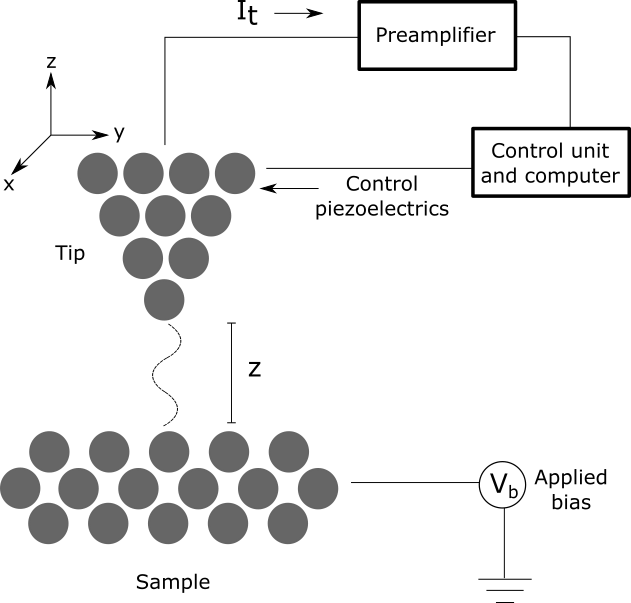
\includegraphics[width=0.6\textwidth]{pictures/stm_diagram.png}
    \caption{Schematic of STM system.}
    \label{fig:exptech:stmsetup}
\end{figure}

\sloppy An approximation of the tunnelling current could be gathered from a \ac{1D} one particle model (\autoref{fig:exptech:wkb}). The solutions of the Schr\"odinger equation in the tip and sample regions would give free-electron wave functions\footnote{Electrons in a metal are assumed behave like free particles.}, while inside the barrier---the vacuum gap between tip and sample---would give wave function $\psi(z) \propto e^{-kz}$, with $k^2 = 2m({U_B(z,V_b) - E})/\hbar^2$, where $U_B(z,V_b)$ is the barrier potential and $E$ is the energy of the tunnelling electron. For electrons with energies high enough and tip-sample distance $z$ small enough, the wave function would be non-zero on the other side of the barrier. From the \ac{1D} \ac{WKB} approximation, the probability of transmission is
\begin{equation} \label{eq:exptech:transfcn}
T(z,E,V_b) = \exp{\left(-2\int_{z_1} ^{z_2} k dz \right)} = \exp{\left(-2  \int_{z_1}^{z_2} \sqrt{\frac{2m}{\hbar^2}\left(U_B(z,V_b) - E\right)} dz \right)}.
\end{equation}
 The barrier potential is unknown, and is often assumed be a trapezoidal barrier, as shown in \autoref{fig:exptech:wkb}. For experimental analysis, the trapezoidal barrier is further approximated by a rectangular barrier of height $U_B(V_b) = (\Phi_t + \Phi_s + eV_b)/2$, which holds when bias voltages are low. For a constant bias voltage in \ac{STM}, the transmission probability in \autoref{eq:exptech:transfcn} decays exponentially, giving tunnelling current $I_t \propto e^{-2kz}$ sensitive to changes in tip-sample distance. This sensitivity allows for picometre height resolution, while a sharp tip allows for sub-nanometre lateral resolution imaging.


\begin{figure} [t]
    \centering
    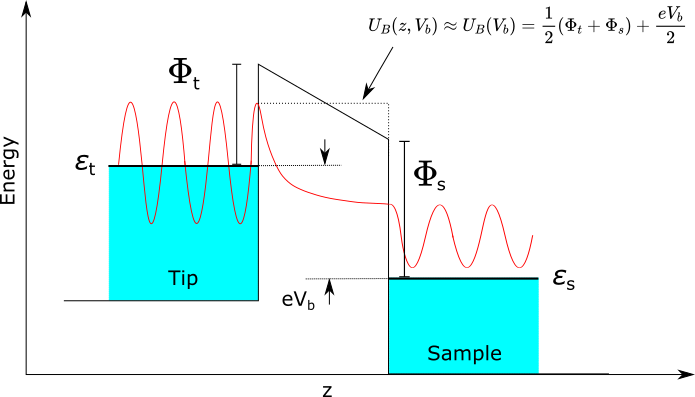
\includegraphics[width=0.9\textwidth]{pictures/wkb.png}
    \caption{Schematic of 1D tunnelling between tip and sample. Wave functions in the tip and sample are oscillatory, and exponentially decaying in the vacuum barrier. A positive bias allows electrons under the tip Fermi energy $\varepsilon_t$ to tunnel into states above the sample Fermi energy $\varepsilon_s$.
    A trapezoidal barrier is often approximated with a constant potential based on the average work function and the bias energy.}
    \label{fig:exptech:wkb}
\end{figure}

%In both modes, the bias voltage is held constant. 
There are two modes of \ac{STM} operation: the constant height, and the constant current mode. In constant height mode, the tip-sample distance is held constant while the tip is rastered across the sample. The corresponding variations in the tunnelling current is measured as a function of the spatial variables. A drawback of this mode is the possibility of crashing the tip into the sample due to tall features on the surface, damaging both the tip and the sample. Alternatively, constant current mode holds the tunnelling current constant by using a feedback loop to adjust the tip height as it scans across the sample. In this case, the tip height is recorded as a function of the lateral $(x,y)$ positions of the tip, giving a tunnelling current isosurface plot (\autoref{fig:exptech:stmexample}), typically referred to as the topography. All \ac{STM} images presented in this thesis are obtained in constant current mode.

\begin{figure} [h]
    \centering
    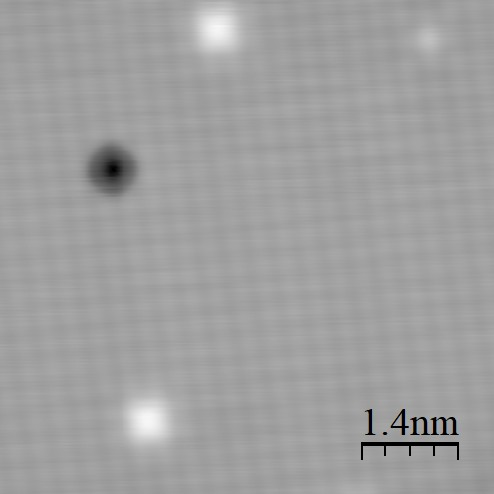
\includegraphics[width=0.45\textwidth]{pictures/atomic_NaCl.jpg}
    \caption[Constant current STM image of bilayer NaCl on Ag(111) (\stmparams{7}{7}{-1}{100}). The atoms of the NaCl(001) lattice are resolved, with the bright spots corresponding to the \ch{Cl-} ions. Various defects are observed on the lattice.]{Constant current STM image of bilayer NaCl on Ag(111) (\stmparams{7}{7}{-1}{100}). The atoms of the NaCl(001) lattice are resolved, with the bright spots corresponding to the \ch{Cl-} ions \citep{heidorn2013influence}. Four defects of various kinds are observed on the lattice.}
    \label{fig:exptech:stmexample}
\end{figure}

% also talk about how to interpret the data, not exactly a physical topography
An \ac{STM} image should not be interpreted as a physical topography. The tunnelling current is dependent on both the tip-sample height and the \ac{LDOS} of the sample. More details on the tunnelling current are given in \autoref{sec:exptech:sts}.




%%%%%
\section{Scanning tunnelling spectroscopy}
\label{sec:exptech:sts}

\Acf{STS} is a technique similar to \ac{STM}, but allows for energetic resolution of the \ac{LDOS} of the sample. At a point over the sample, the tip is held at a constant height and the current feedback loop is turned off. The tunnelling current is then measured as the bias between tip and sample is swept across a range of values. For studying organic molecules, the bias typically ranges from $\SI{-3}{V}$ to $\SI{3}{V}$, depending on the molecular stability and the energies at which the orbital features are found.

The relationship between the current signal, $I(V)$, and the \ac{LDOS} can be understood by returning to the \ac{1D} tunnelling model (\autoref{fig:exptech:stsldos}). The tip is assumed to have a constant density of states. The bias voltage shifts the energy of the electrons in the tip relative to those of the sample. At positive biases, the Fermi level\footnote{The Fermi level is the electrochemical potential of the material, or the energy at which there is 50\% state occupation at finite temperatures. This is not to be confused with the Fermi energy, which is defined for $T=\SI{0}{K}$. The terms will be used interchangeably, as our experimental condition is close to absolute zero.} of the tip shifts up, allowing electrons to tunnel into the unoccupied states of the sample. Conversely, at negative biases, the Fermi level of the tip shifts down, allowing electrons to tunnel from the occupied sample states into the tip. Changes in the sample density of states $\rho_s(E)$, both occupied and unoccupied, will open new tunnelling channels that are reflected in changes in the measured $I(V)$. More details on the tunnelling current and the recovery of the density of states are described in the below sections.

\begin{figure} [h]
    \centering
    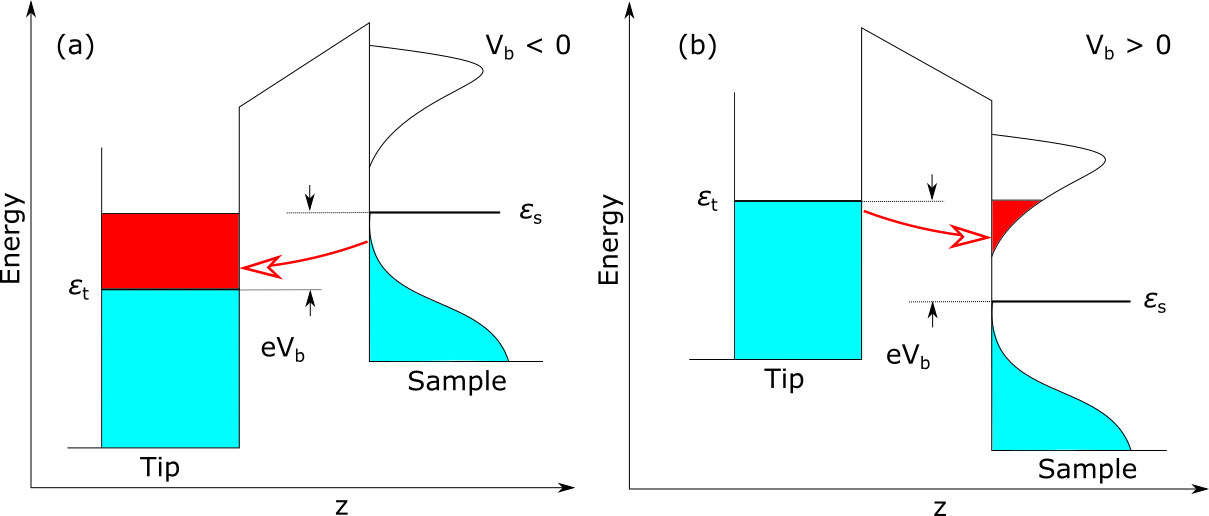
\includegraphics[width=0.9\textwidth]{pictures/sts_ldos.png}
    \caption{Schematic showing the tunnelling process as a function of bias voltage. \textbf{(a)} For positive bias voltages, the sample Fermi energy is below the tip Fermi energy. The resulting current arises from electrons of the occupied tip LDOS tunnelling into the sample. \textbf{(b)} At negative bias voltages, the reverse process occurs, and electrons in the sample tunnel into the unoccupied tip LDOS.}
    \label{fig:exptech:stsldos}
\end{figure}

The technique can be further extended by performing \ac{STS} pixel-by-pixel in a grid, giving a spatial map of the \ac{LDOS} over an area of the sample. This is done in conjunction with \ac{STM}, with the tip pausing at grid points for \ac{STS} spectra, before resuming the \ac{STM} scan. The added time for pixel-by-pixel spectra means that \ac{STM}/\ac{STS} grids can take hours or days to complete, during which changes in the sample or the tip can affect measurements. 


\subsection{Tunnelling theory}
% \FIXME{Add Bardeen, Tersoff and Hamann, Feuchtwang, Caroli et al., JB Pendry, Gottlieb and Wesoloski citations.}
In order to extract quantitative information from \ac{STS}, we must understand the theory of quantum tunnelling, and its application to the tip-sample configuration of the experiment. The first theoretical formulation of many particle tunnelling was developed by \textit{Bardeen} in 1960, using what was called a ``transfer Hamiltonian" \citep{PhysRevLett.6.57}. It was then applied to \ac{STM}/\ac{STS} by \textit{Tersoff and Hamann} \citep{0957-4484-17-8-R01,tersoff1985theory}. 

Bardeen's formulation does not take into account many-body effects, strong tip-sample interactions, and strong tunnelling. To date, the most rigorous analytic tunnelling theory is formulated using \acp{NEGF}, first developed by \textit{Feuchtwang} and later expanded upon by \textit{Pendry et al.}, which can address the short-comings of the transfer Hamiltonian \citep{feuchtwang1974tunneling, pendry1991theory}. However, the transfer Hamiltonian formulation is sufficient for extracting the \ac{LDOS} from \ac{STS} data, with the conditions for validity approximated in experiment. Furthermore, the \ac{NEGF} tunnelling theory has been demonstrated to be reducible to Bardeen's tunnelling theory, and thus, this section will discuss the transfer Hamiltonian approach to tunnelling \citep{0957-4484-17-8-R01}.

% taken from Guide on tunnelling Theory
In assuming that the tip and sample are independent, with weak interactions between them, we can define the sample and tip Hamiltonians separately as
\begin{align}
H_{s}\psi(\pmb{r}) &= -\frac{\hbar^2}{2m} \nabla^2 \psi(\pmb{r}) + V_{s}(\pmb{r}) \psi(\pmb{r}), \\
H_{t}\phi(\pmb{r}) &= -\frac{\hbar^2}{2m} \nabla^2 \phi(\pmb{r}) + V_{t}(\pmb{r}) \phi(\pmb{r}) ,
\end{align}
where $V_s$(\pmb{r}) and $V_t$(\pmb{r}) are the sample and tip potentials, respectively; $\psi(\pmb{r})$ and $\phi(\pmb{r})$ are eigenstates bounded to the sample and tip, respectively. We can also define a Hamiltonian of the entire system responsible for the transfer of electrons between the tip and sample (the so called ``transfer Hamiltonian")
\begin{equation} \label{eq:exptech:transH}
H\Psi = - \frac{\hbar^2}{2m} \nabla^2 \Psi + V(\pmb{r}) \Psi \quad \textrm{where} \quad V(\pmb{r}) = 
\begin{cases}
V_t(\pmb{r}) & \textrm{ in tip} \\
V_t(\pmb{r}) + V_s(\pmb{r}) & \textrm{ in barrier} \\
V_s(\pmb{r}) & \textrm{ in sample}
\end{cases},
\end{equation}
where $\Psi(\pmb{r})$ are the eigenstates of the transfer Hamiltonian, and the potentials of the tip and sample only overlap in the vacuum barrier region.

\sloppy Consider an initial sample state\footnote{The spatial $\pmb{r}$ dependence of the states are implied, and dropped from the notation.} $\psi(t=0)$ which satisfies the eigenvalue equation $H_{s}\psi(0) = \epsilon \psi(0)$. When tunnelling is weak enough, then for some small time $t$ the sample states would be given by $\psi(t) = e^{-itH_{s}/\hbar} \psi(0) = e^{-it\epsilon/\hbar} \psi(0) $. For all $t$, assuming that tunnelling is weak, we expand over the tip states $\phi_k$ satisfying the eigenvalue equation $H_{t}\phi_k = \xi_k \phi_k$
\begin{equation} \label{eq:exptech:state}
\psi(t) = e^{-it\epsilon/\hbar} \psi(0) + \sum_k a_k(t) \phi_k,
\end{equation}
where $a_k$ are coefficients of the expansion. Since there is no tunnelling initially, there would be no contribution from the tip state, and for all $k$ the coefficients vanish at $t=0$. By approximating $a_k(t)$, we can take the time derivative to look at the rate of ``transfer" from the initial sample state to the tip state, and from that the tunnelling current.

By plugging the state (\autoref{eq:exptech:state}) into the time-dependent Schr\"odinger equation of the transfer Hamiltonian (\autoref{eq:exptech:transH}), and separately taking the time derivative, we have two expressions for $\frac{\partial \psi}{\partial t}$. Equating gives us
\begin{equation}
i\hbar \sum_k \frac{d}{dt} a_k(t) \phi_k = e^{-it\epsilon / \hbar} (H-H_{s})\psi(0) + \sum_k a_k(t) (\xi_k \phi_k + (H-H_{t})\phi_k),
\end{equation}
where $H$ is the transfer Hamiltonian, and $\xi_k$ are the eignenenergies of the tip states. Taking the inner product with $\phi_j$, for any $j$-th tip state
\begin{equation} \label{eq:exptech:scatteringprob}
i\hbar \frac{d}{dt} a_j(t) = e^{-it\epsilon/\hbar} \Bra{\phi_j}H-H_{s} \Ket{\psi} + \xi_j a_j(t) + \sum_k a_k(t) \Bra{\phi_j} H - H_{t} \Ket{\phi_k}.
\end{equation}

Due to weak tunnelling, for a little while ($t \ll 1$), $a_j(t)$ is the only non-zero coefficient, and the last term of \autoref{eq:exptech:scatteringprob} vanishes. The resulting differential equation has solutions
\begin{equation}
a_j(t) =  \frac{e^{-it\epsilon/\hbar} - e^{-it\xi_j/\hbar}}{\epsilon - \xi}  \Bra{\phi_j} H-H_{s} \Ket{\psi}.
\end{equation}
For rate of scattering from the sample into the tip as a result of the transfer Hamiltonian (\autoref{eq:exptech:transH}), calculate the total $\sum_k \abs{a_k(t)}^2$ and take the time derivative
\begin{equation}
\frac{d}{dt}\sum_k |a_k(t)|^2 = \frac{d}{dt}  \sum_k \frac{t^2}{\hbar^2}\textrm{sinc}^2 \left(\frac{t(\xi_k - \epsilon)}{2\hbar} \right) | \Bra{\phi_k} H-H_{s} \Ket{\psi}  | ^2.
\end{equation}

For sufficiently large $t$, the sinc function can be approximated as the Dirac $\delta$-function. For a continuous \ac{DOS}, the summation over $k$ becomes an integral over all energies, and the integral can be evaluated

\begin{align}
\frac{d}{dt}\sum_k |a_k(t)|^2 &\approx  \frac{d}{dt}  \int_{-\infty}^\infty dE \left[ \frac{\pi t^2}{\hbar^2} \delta \left(\frac{t(E - \epsilon)}{2\hbar} \right) | \Bra{\phi_E} H-H_{s} \Ket{\psi}  | ^2 \right], \\
&\approx  \frac{2\pi }{\hbar} \rho_t(\epsilon) \abs{\mathfrak{M}}^2,
\end{align}
where $\rho_t(\epsilon)$ is the tip density of states near $\epsilon$, the eigenenergy of the sample state $\psi$. The equation above is also known as Fermi's Golden Rule. The matrix element $\abs{\mathfrak{M}}^2 = \abs{\Bra{\phi_\epsilon} H - H_s \Ket{\psi}}^2$ is the transition probability of the sample state into a tip state near $\epsilon$, denoted as $\phi_\epsilon$.

To get the tunnelling current, we look to the work of Tersoff and Hamann, considering tunnelling from either side of the junction. We continue to assume independent sample and tip and weak tunnelling, such that the addition or removal of electrons does not greatly affect the chemical potentials of the tip and sample, $\mu_t$ and $\mu_s$ respectively. We will also assume a low bias so that band-bending is negligible.

In these limits, the statistics of the electrons are governed by the Fermi-Dirac distribution: at temperature $T$ and chemical potential $\mu$, the probability of finding an electron at energy $E$ is $F_{\mu, T}(E) = ({e^{(E-\mu)/k_BT} +1})^{-1}$. The tunnelling of electrons \emph{from} a \emph{filled} sample state $\psi_n$ with energy $\epsilon_n$ into an empty tip state would be
\begin{equation} \label{eq:exptech:Is->t}
    I_{s\rightarrow t} = \frac{2\pi e}{\hbar} \sum_n F_{\mu_s, T}(\epsilon_n) (1-F_{\mu_t, T}(\epsilon_n))  \rho_{t}(\epsilon_n) \abs{\mathfrak{M}}^2 ,
\end{equation}
where $e$ is the elementary charge. The tunnelling of electrons \emph{into} an \emph{empty} sample state $\psi_n$ from filled tip states near energy $\epsilon_n$ would be 
\begin{equation} \label{eq:exptech:It->s}
    I_{t\rightarrow s} = \frac{2\pi e}{\hbar} \sum_n (1-F_{\mu_s, T}(\epsilon_n))   F_{\mu_t, T}(\epsilon)  \rho_{t}(\epsilon_n) \abs{\mathfrak{M}}^2 .
\end{equation}

% Since the bais was defined relative to the sample, the current from the tip to sample is defined as positive, and from the sample to tip as negative. 
The difference between the expressions in \autoref{eq:exptech:Is->t} and \ref{eq:exptech:It->s} will give the total tunnelling current. Rewriting the total current by referencing the energy $\epsilon_n$ with respect to the Fermi level of the sample, which is biased lower than the tip energy by $eV_b$, we have
\begin{equation} 
I = \frac{2\pi e}{\hbar}\sum_n f(\epsilon_n, V_b) \rho_{t}(\epsilon_n) \abs{\mathfrak{M}}^2,
\end{equation}
where $ f(\epsilon_n,V_b) = F_{\mu_t=0,T}(\epsilon_n-eV_b) - F_{\mu_s=0,T}(\epsilon_n)$. Note that the Fermi-Dirac equations no longer depend on the chemical potentials of the sample and tip, as they are already accounted for by the bias $eV_b = \mu_t - \mu_s$. 

The entire expression can be approximated by an integral
\begin{equation}
    I \approx \frac{2\pi e}{\hbar} \int_{-\infty}^\infty dE f(E,V_b) \rho_t(E)\rho_s(E) T(E,V_b,z),
\end{equation}
where the matrix elements are approximated by averaging over the sample states $\phi$ near the energy $E$, giving $\abs{\mathfrak{M}}^2 \approx T(z,E,V_b) \rho_s(E)$, where $T(z,E,V_b)$ is the transmission probability in \autoref{eq:exptech:transfcn} .

In the low temperature limit, the Fermi-Dirac equations approach the Heaviside functions, but are thermally broadened at temperatures above absolute zero, limiting the energy resolution of \ac{STS}. Physically, only electrons with energies between the Fermi levels of the sample and tip contribute to the tunnelling current; the expression for the tunnelling current becomes
\begin{equation} \label{eq:exptech:tersoffcurrent}
I_{T \rightarrow \SI{0}{K}} \approx \frac{2\pi e}{\hbar} \int_{0} ^{eV_b} dE \rho_{t}(E) \rho_{s}(E) T(z,E,V_b).
\end{equation}

It is important to remember the limits in which this equation is valid. From Bardeen's formalism, we assume (1) independent tip and sample states, and (2) weak tunnelling. In Tersoff and Hamann's analysis, we further assume (3) Fermi-Dirac statistics, (4) first-order \ac{WKB} tunnelling, (5) low temperatures, and (6) negligible band-bending effects. In general, these conditions hold when the tip and sample are sufficiently far apart, and bias between the two is sufficiently low.


\subsection{Normalization of $dI/dV$}

From the Tersoff and Hamann equation, we can extract the density of states of the sample from the \ac{STS} spectra. In \autoref{eq:exptech:tersoffcurrent}, the current is a convolution of the \ac{DOS} of the tip and sample, and the transmission probability. Assuming that the \ac{DOS} of the tip is featureless, and equal to unity
\begin{equation}
I \propto \int_0 ^{eV} dE \rho_s(E) T(z,E,V) .
\end{equation}
In taking the derivative with respect to the bias voltage\footnote{The subscript in $V_b$ is implied.}, we obtain the differential conductance
\begin{equation} \label{eq:exptech:didv}
\frac{dI}{dV} \propto e \rho_s(E=eV) T(z,E=eV,V) + e \int_0^{eV} dE \rho_s(E) \frac{dT(z,E,V)}{dV}  .
\end{equation}

A commonly used form for the \ac{DOS} of the sample is $\rho_s(E) \propto dI/dV $, where, for small enough biases ($\sim \SI{10}{\milli\electronvolt}$), the integral term in \autoref{eq:exptech:didv} is ignored \citep{feenstra1993methods}. However, for studies of organic semiconductor molecules, features are often found at larger biases ($\sim 1$--$\SI{3}{\electronvolt}$), which would be obscured by the exponential form of the transmission probability (\autoref{eq:exptech:transfcn}). To eliminate the exponential dependence, the differential conductance can be ``normalized" with the conductance  \citep{feenstra1987atom}
\begin{equation} \label{eq:exptech:normdidv}
\frac{dI/dV}{I/V} = \frac{e\rho_s(eV) + e\int_0 ^{eV} dE \frac{\rho_s(E)}{T(z,E=eV,V)} \frac{dT(z,E,V)}{dV}}{ \frac{1}{V} \int_0^{eV} dE \rho_s(E) \frac{T(z,E,V)}{T(z,E=eV,V)}}.
\end{equation}
In this form, the transmission probability appears in ratios with itself, qualitatively cancelling the exponential form. The normalized differential conductance gives the $\rho_s(eV)$ with an additional term arising from interactions of the wave function with the electric field in the junction.

However in \autoref{eq:exptech:normdidv}, divergences arise when we consider $V=\SI{0}{\volt}$ or $I= \SI{0}{\ampere}$. To mitigate this, a small constant term can be added to the conductance without significantly modifying the normalization term \citep{prietsch1991structural}
\begin{equation}
    \overline{I/V} = \sqrt{(I/V)^2 + c^2},
\end{equation}
where for constant $c\ll I/V$ we would have $\overline{I/V} \approx I/V$ to the first order. For \ac{STS} data analysed in this thesis, all \ac{DOS} is approximated by $ (dI/dV) / (\overline{I/V})$.

%%%%%
\section{Scanning tunnelling microscopy luminescence}

% allows us to probe the excited states of molecules on surface
In the \ac{STM} setup, an optical system can be integrated to allow for detection of tunnelling induced luminescence. This mode of operation is known as \acf{STML}. The tip acts as a source of electrons and holes that can locally excite photon emission from the sample \citep{gimzewski1988photon}, thus allowing the near-field study of luminescence from nanoscale structures on metals, semiconductors, and molecules \citep{Qiu2003}. The intensity and spectral distribution of the photons provide information on the optical properties of the material, as well as inelastic tunnelling processes which would otherwise be undetectable in \ac{STM} or \ac{STS} \citep{novotny2012principles}. Additionally, with organic semiconductor molecules, vibrational states can be seen in the photoemission spectra, particularly in the visible and infrared ranges \citep{Qiu2003,Wu2008}.

To perform \ac{STML}, there must be optical access to the tip-sample junction of the \ac{STM}, which acts as a point source of emission. A lens mounted to the microscope head is focused at the junction, collimating the emission. An optical path through several windows and viewports allows the photons to exit the microscope and be refocused by an exterior lens into a detector, such as a spectrometer. 

% The spectrally resolved photons give information on the excited states and vibrational modes of the molecule. Combined with the high spatial resolution of the \ac{STM}, emission and absoprtion spectroscopy can be carried out on single molecules in the optical near-field regime. With \ac{STML}, a real-space nanoscale understanding of the electromagnetic coupling of \ac{OLED} and \ac{OPV} molecules can be achieved.

Emission from the tunnelling junction can be described by two main processes: (1) the excitation of the free electron gas in the metallic substrate, and (2) the fluorescence of a quantum confined system---such as an organic semiconductor molecule. The subsequent sections will describe both processes in further detail. 


\subsection{Plasmon emission}

The first observations of tunnelling induced luminescence were seen in metal-oxide-metal junctions in 1976, by Lambe and McCarthy \citep{lambe1976light}. Later experiments on metal surfaces \citep{berndt1991inelastic, ushioda1992stm, hoffmann2002color} demonstrated that the same effect can be seen in \ac{STM}. While there are other proposed mechanisms, the emission is generally attributed to the decay of plasmons excited by \acf{IET} processes \citep{berndt1991inelastic}.

Inelastic processes in tunnelling typically account for about 1\% of the total current \citep{novotny2012principles}. In \ac{IET}, the tunnelling electrons or holes lose a fraction of energy to an excitation, such as phonons or plasmons  \citep{vitali2004phonon}. Plasmon excitation occurs when the tunnelling electrons excite charge oscillations in the substrate. Plasmons at the interface between the metallic substrate and the vacuum can couple to the electromagnetic field, becoming \acp{SPP}, which then decay into photons.\footnote{Although no plasmons are physically emitted, due to the origin of the emissions, I will refer to the photons as ``plasmon emission.''} 

% In some models, the inelastic process occurs \emph{after} elastic tunneling, when the electron thermalises (release energy) which then excites the \ac{SPP}. This is known as \acf{HET}. In metals and indirect-gap semiconductors, \ac{HET} is negligible compared to \ac{IET}, with theoretical estimates putting the quantum efficiency, the photons emitted per charge carrier, of \ac{IET} two orders of magnitude higher. However in direct-gap and organic molecular semiconductors, \ac{HET} may be the primary mechanism for luminescence.

\begin{figure} [h]
    \centering
    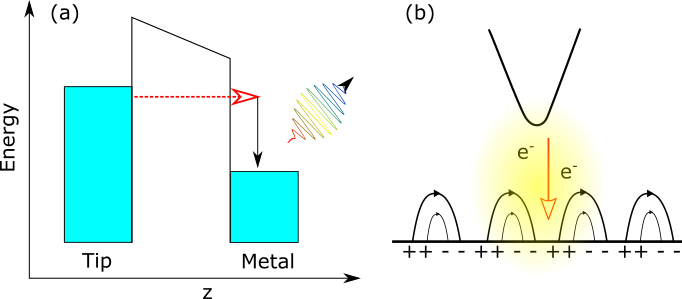
\includegraphics[width=\textwidth]{pictures/spp_emission.png}
    \caption{ Diagram of excitation of SPP through inelastic tunnelling. The process is possible at negative biases as well. \textbf{(a)} Electrons tunnel inelastically into the sample. The energy excites a surface plasmon which decays to give emission. \textbf{(b)} Energy from hot electron convert into charge oscillations and associated electromagnetic fields. Plasmons localized to the surface become SPPs. }
    \label{fig:exptech:iet-het}
\end{figure}

\subsection{Organic molecule emission}

In a quantum-confined system such as an organic semiconductor molecule, luminescence is seen due to the recombination of excitons formed in the semiconductor gap. Excitons are excited electrons that are bound by the Coulomb force to the positively charged ``holes" left behind. Recombination is the process in which the excited electron falls back into the hole, emitting the energy as a photon. In organic photovoltaics, recombination should be minimized in order to increase the power conversion efficiency of the device. However, in light emitting applications, recombination is necessary, but the optical gap and the emission energy needs to be finely tuned. Using \ac{STML}, exciton physics of the organic semiconductors can be studied at atomic-resolution, in relation to the geometric configuration and electronic environment of the molecule.

There are two generally accepted mechanisms for exciton generation in organic molecules (\autoref{fig:exptech:2-mechanisms}): plasmon-mediated, and charge injection. Plasmon-mediated exciton formation involves the photoexcitation of electrons in the semiconductor by plasmonic emission. In this mechanism, the energy of the plasmon emission needs to be greater than the \ac{HOMO}-\ac{LUMO} gap in an organic molecule. 

In charge injection exciton formation, electrons directly tunnel into the unoccupied state of the organic semiconductor, while an electron tunnels out of the occupied state into the substrate, effectively injecting a hole into the molecule. The electron-hole pair can then form and recombine to emit a photon. The charge injection mechanism requires an insulating barrier between the molecule and the substrate to allow for a shift in the substrate Fermi level that is (relatively) independent of the molecular energy states. Additionally, the tip-sample bias needs to be high enough that the tip and sample Fermi levels allow for simultaneous electron and hole injection. The rate of exciton formation would depend on the rate of charge tunnelling through the vacuum and insulating layer barriers.

Charge injection is generally accepted as the primary mechanism for luminescence of organic molecules in \ac{STML}, however, evidence for plasmon-mediated mechanisms has been seen in some experiments \citep{uemura2007local, Dong2010, zhang2012tip}. It is possible that the emission comes from a combination of both mechanisms.

% Because the thermalisation occurs after elastic tunnelling, the charge injection process is analagous to \ac{HET}, and is generally accepted the primary mechanism for luminescence of organic molecules in \ac{STML}, however, evidence for the plasmon-mediated mechanism have been seen in some experiments.



\begin{figure} [H]
    \centering
    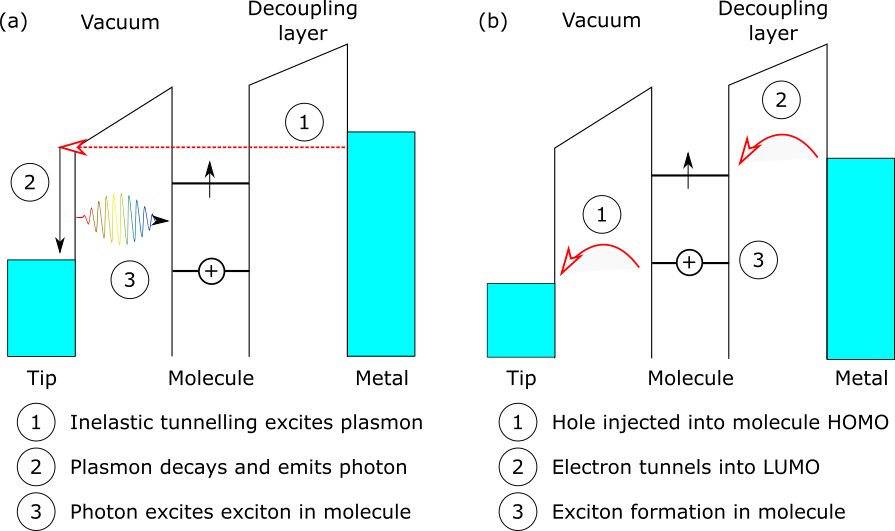
\includegraphics[width=0.9\textwidth]{pictures/exciton_mechanisms.png}
    \caption[Energy diagrams to describe two different exciton formation mechanisms of an organic molecule. \textbf{(a)} Plasmon-mediated and \textbf{(b)} charge injection exciton formation.]{Energy diagrams to describe two different exciton formation mechanisms of an organic molecule. \textbf{(a)} Plasmon-mediated and \textbf{(b)} charge injection exciton formation. Figure adapted from \citep{kuhnke2017atomic}. }
    \label{fig:exptech:2-mechanisms}
\end{figure}



\subsection{Experimental factors}

The success of an \ac{STML} experiment is dependent on many factors, such as the material of the tip and sample, the geometry of the tip, and the optical properties of the molecule.

For strong luminescence from tunnelling electrons, the tip and sample should be composed of materials with low dielectric loss in the wavelength region of interest. Organic semiconducting molecules typically have optical gaps of 1\SI{-3}{eV}, resulting in exciton emission in the visible/IR range. \ac{STML} study of organic molecules should be performed with tip and sample composed of noble metals silver (Ag) \citep{yang2015optical} and gold (Au) \citep{olmon2012optical}. Low dielectric loss means that the electric field can more easily penetrate the material, and the conduction electrons in the metal can move more freely within the bulk, allowing for stronger plasmonic response \citep{novotny2012principles}. Oxide layers or other contaminants can quench emissions from the tip-sample junction.

The tip geometry is crucial to maximizing signal-to-noise ratio in \ac{STML}. Luminescence signals can be enhanced by the plasmonic nano-cavity formed by the tip and the sample, an effect known as Purcell enhancement \citep{purcell1946spontaneous}. Typical emission rates from semiconducting molecules in \ac{STML} are $\sim 10^{-5}$--$10^{-3}$ photons per electron \citep{johansson1998light, zhang2011fabrication}. The coupling of the exciton and the plasmon can increase the strength of the organic molecule \ac{STML} signal by up to five orders of magnitude \citep{chen2015molecular}. Theoretical simulations have determined that stronger plasmonic response is seen in sharper tips due to the enhancement of electric fields at the tip apex by the lightning rod effect \citep{novotny2012principles, aizpurua2000role}. Experimentally, the exact tip geometry cannot be determined, however, small changes to the tip apex can change the energy and strength of the plasmon emission dramatically \citep{meguro2002origin}. For our experiment, the tip was pulsed and indented until the detected plasmon emission is strong, featureless, and broad. More details on tip preparation are presented in \autoref{sec:expsetup:tip_prep}.

The molecules should possess a high quantum efficiency---the ratio of photons emitted per charge carrier---and high stability on the surface, especially under the strong electromagnetic fields in the tip-sample junction. Typical \ac{STML} conditions at $V_b \sim \SI{2}{V}$ and $I_t \sim \SI{100}{pA}$ would give tip-sample distances $\sim \SI{5}{\angstrom}$ \citep{Qiu2003}, and electric fields $\sim \SI{1}{V/nm}$ \citep{grosse2014dynamic}.  Regardless of the prevalent mechanism for \ac{STML} on organic molecules, molecule-substrate interactions should be minimized to prevent quenching of luminescence due to additional energetic pathways for the excitation to relax \citep{kuhnke2017atomic, rossel2010fluorescence}. This is usually done by using a thin insulating layer between the molecule and substrate, such as metal-oxide or NaCl layers. 









\endinput








\subsection{garbage}
\begin{equation}
    I_t \propto e^{-2kz},
\end{equation}

where $k$ is 

Has proven to be powerful in understanding the topological and electronic features of surfaces near the atomic level. 

The works \citep{tersoff19931} of \textit{Young et al.}, with the creation of the topografiner, and \textit{Teague}, with the demonstration of vacuum tunnelling between gold electrodes, preceeded the invention of \ac{STM}. The topografiner used a piezoelectric driver to scan surfaces with a probe at small distances, advancing the technology required for the \ac{STM}. Teague's experiments revealed the possibility of vacuum tunnelling, at the voltages and gap widths used today in \ac{STM}. 

\ac{STM} is based on the quantum tunnelling of electrons through a potential barrier. In experiment, a tip is brought close to the sample of interest. A bias is applied to the system to allow for tunnelling, and the measured current gives information about the sample's \ac{LDOS}. The tip-sample distance is usually around 5 to 15 Angstroms, with the tunnelling current in the nano-ampere range. The voltage applied can range from 10mV to 10V in either directions.


Here, we notice that $P_t$ is the sinc function, which contributes to the integral mostly in the region of $[-2h/t, 2h/t]$. So as $t$ grows, the interval becomes smaller and smaller, until the tip energy $E_k$ can be approximated to be constantly distributed in the interval. The sum can then be approximated to be an integral, with $\rho_{tip}(\epsilon)$ being the number of tip states near the energy of the sample state $\epsilon$, 
\begin{align}
\sum_k P_t(E_k - \epsilon) \abs{\mathfrak{M}}^2 &\approx \abs{\mathfrak{M}}^2(\psi) \rho_{tip}(\epsilon) \int_{-2h/t}^{2h/t} P_t(E) dE \\
& \approx \abs{\mathfrak{M}}^2(\psi) \rho_{tip}(\epsilon) \int_{-\infty}^{\infty} P_t(E) dE = \abs{\mathfrak{M}}^2(\psi) \rho_{tip} \frac{\pi t}{2\hbar}.
\end{align}
Finally, the scattering rate (or the transition probability) is given by
\begin{equation}
\frac{d}{dt} \sum_k |a_k(t)|^2 \approx \frac{d}{dt}\left( \frac{2\pi t}{\hbar} \abs{\mathfrak{M}}^2(\psi) \rho_{tip}(\epsilon) \right) = \frac{2 \pi}{\hbar} \abs{\mathfrak{M}}^2(\psi) \rho_{tip}(\epsilon).
\end{equation}

can excite localised charge oscillations known as \acp{TIP} in metallic substrate. At the interface between the substrate and the vacuum, the \ac{TIP} mode can become electromagnetically coupled, creating \acp{SPP} which propagate parallel to the interface. Upon decay of the \ac{SPP}, photons are radiated. This process is dominant in 

Theoretical studies estimate the inelastic tunnelling accounts for about 1\% of the total current,  where elastic tunnelling dominates the signal. Of the \acp{TIP} generated by inelastic tunnelling, only about 10\% couple with the electromagnetic field, yielding photon counts of $\sim 10^{-4}$ per tunnelled carrier. To maximise this signal, there are two main experimental considerations: the shape of the tip, and the material of the tip and sample.


% experimental setup
%% The following is a directive for TeXShop to indicate the main file
%%!TEX root = diss.tex

\chapter{Experimental Setup and Simulation Methods}
\label{ch:expsetup}

In this chapter, I will discuss the instrument and optical setup used, along with details on sample and tip preparation. I will also discuss the \ac{DFT} details, including the software package, potential approximation method, and basis set used. The results of the \ac{DFT} calculation are qualitatively compared with the experimental results.

%\section{Low vibration facility}

\section{The microscope}

All experimental measurements were made on an Omicron \ac{UHV} \ac{LT} \ac{SPM} (\autoref{fig:expsetup:omicron}). Experimental data was obtained at \ac{LHe} temperatures ($\sim \SI{4.3}{K}$) and at pressures around $1 \times 10^{-11}$ mbar. 

\begin{figure} [h]
    \centering
    %\includegraphics[width=3in]{file}
    \caption{\FIXME{Image of the microscope.}}
    \label{fig:expsetup:omicron}
\end{figure}

The entire microscope is inside of an ultra-low vibration facility (dubbed ``the pod"), where it sits on a \SI{36}{tonne} inertial concrete block that is resting on six pneumatic isolators. To further decouple vibrations from the main building from the microscope, the pod is surrounded by a double-walled concrete enclosure containing acoustically isolating material, and rests on a foundation separate from the main building. Small feed-through openings allow wires to be passed from the microscope to a control unit outside the pod. The microscope can then be remotely operated using a computer in a separate control room. More details on the performance and design of the ultra-low vibration facility is given in reference \citep{macleod2015ultra}.

The microscope is composed of two main chambers: the preparation and the \acf{LT} chamber. The preparation chamber is typically at a base pressure of $\sim 1\times 10^{-10}$ mbar, minimizing contamination during sample preparation. In this chamber, the metallic substrates are cleaned by repeated sputtering and annealing. Decoupling layers of \ch{NaCl} can then be deposited onto the surface using a home-built Knudsen evaporator. The substrates are then transferred into the \ac{LT} chamber for imaging and experimentation.

The \ac{LT} chamber is separated from the preparation chamber by a gate valve, and has a base pressure of $\sim 1\times 10^{-11}$ mbar. Samples are often stored in this chamber on a rotating carousel, due to the cleanliness and lower pressure. The samples can be loaded into the \ac{SPM}, which is kept at $\sim \SI{4.3}{K}$ by a cryostat of \acf{LHe} surrounded by a \acf{LN2} bath. With the sample inside the \ac{SPM}, molecules are thermally deposited on the cold sample using an \ac{OMBE} evaporator. At such low temperatures, the molecules are more stable on insulating \ch{NaCl} layers, and less diffusive, preventing aggregation and self-assembly \FIXME{citation}. A ceramic heater in the sample stage allows for annealing in the \ac{LT} chamber. For more information on the equipment in the chambers, including the evaporators, and the sample design, refer to \citep{cochrane2017single, roussy2016coupling}. 



\subsection{Scanning probe with optical access}

The imaging \ac{SPM} head is shown in \autoref{fig:expsetup:head}. The entire apparatus is suspended on damping springs, which can be clamped to the cryostat for sample transfer and faster cooling. The tip sits on a scanner, which is controlled by a coarse motor and piezoelectric motors. To begin an experiment, the tip is brought visually  to the sample using the coarse motor. An auto-approach function is then activated, taking a coarse step and extending the piezoelectric motor repeatedly until a tunnelling current is detected.

\begin{figure} [h]
    \centering
    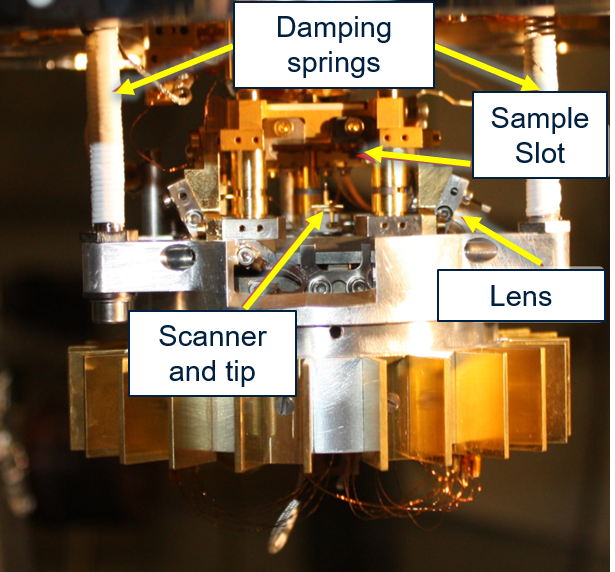
\includegraphics[width=2.5in]{pictures/head.png}
    \caption{\FIXME{STM head.}}
    \label{fig:expsetup:head}
\end{figure}

There are two ports for optical access to the \ac{SPM} head. A camera used for coarse tip approach occupies one, while a home-built lens tube used for \ac{STML} occupies the other. A planoconvex sapphire lens (Melles-Griot) sits inside the lens tube, about \SI{18}{mm} from the tip-sample junction, at an angle of \SI{25}{\degree} from the sample. This geometry allows for collection of photons in about 5\% of the half solid angle above the sample. In order to maximize photon collection, the lens is focused at the tip-sample junction for the Ag(111) substrate. The tip-sample junction is well approximated as a point source of light, and any shift from the lens focal point can broaden and weaken spectral features. When using the Au(111) thin film substrate, the height of the sample is different resulting in weaker \ac{STML} signals.
% PXS-10.0-15.4-S

The light from the lens then passes through ports in the two heat shields. These ports have KG5 \ac{IR} filters (SCHOTT) situated inside to reduce radiative heating of the \ac{SPM} head, and reduction in cryostat hold time. Photon emission from organic semiconductor are often in the visible to near-\ac{IR} range, so the filters were later replaced with a WG41050 bandpass filter  (ThorLabs) that transmits wavelengths up to \SI{1000}{nm}. The transmission curves of the filters are shown in \autoref{fig:expsetup:windows}. To counteract increased thermal energy entering the heat shields, the inner heat shield port opening was reduced from \SI{20}{mm} to \SI{12}{mm} in diameter using a \SI{0.4}{mm} thick gold-plated BeCu plate. After replacement of the filter, no noticeable changes were seen in the cryogenic hold time. \emph{All \ac{STML} data was taken with the KG5 \ac{IR} filters in place}. Due to time constraints, \ac{STML} measurements were not repeated after the new window system was installed. The photons finally exit the \ac{LT} chamber through a Kodial vacuum viewport (VacGen), where they then enter an external optical setup mounted on the microscope. 
\begin{figure} [h]
    \centering
    \begin{subfigure}{.5\textwidth}
        \centering
        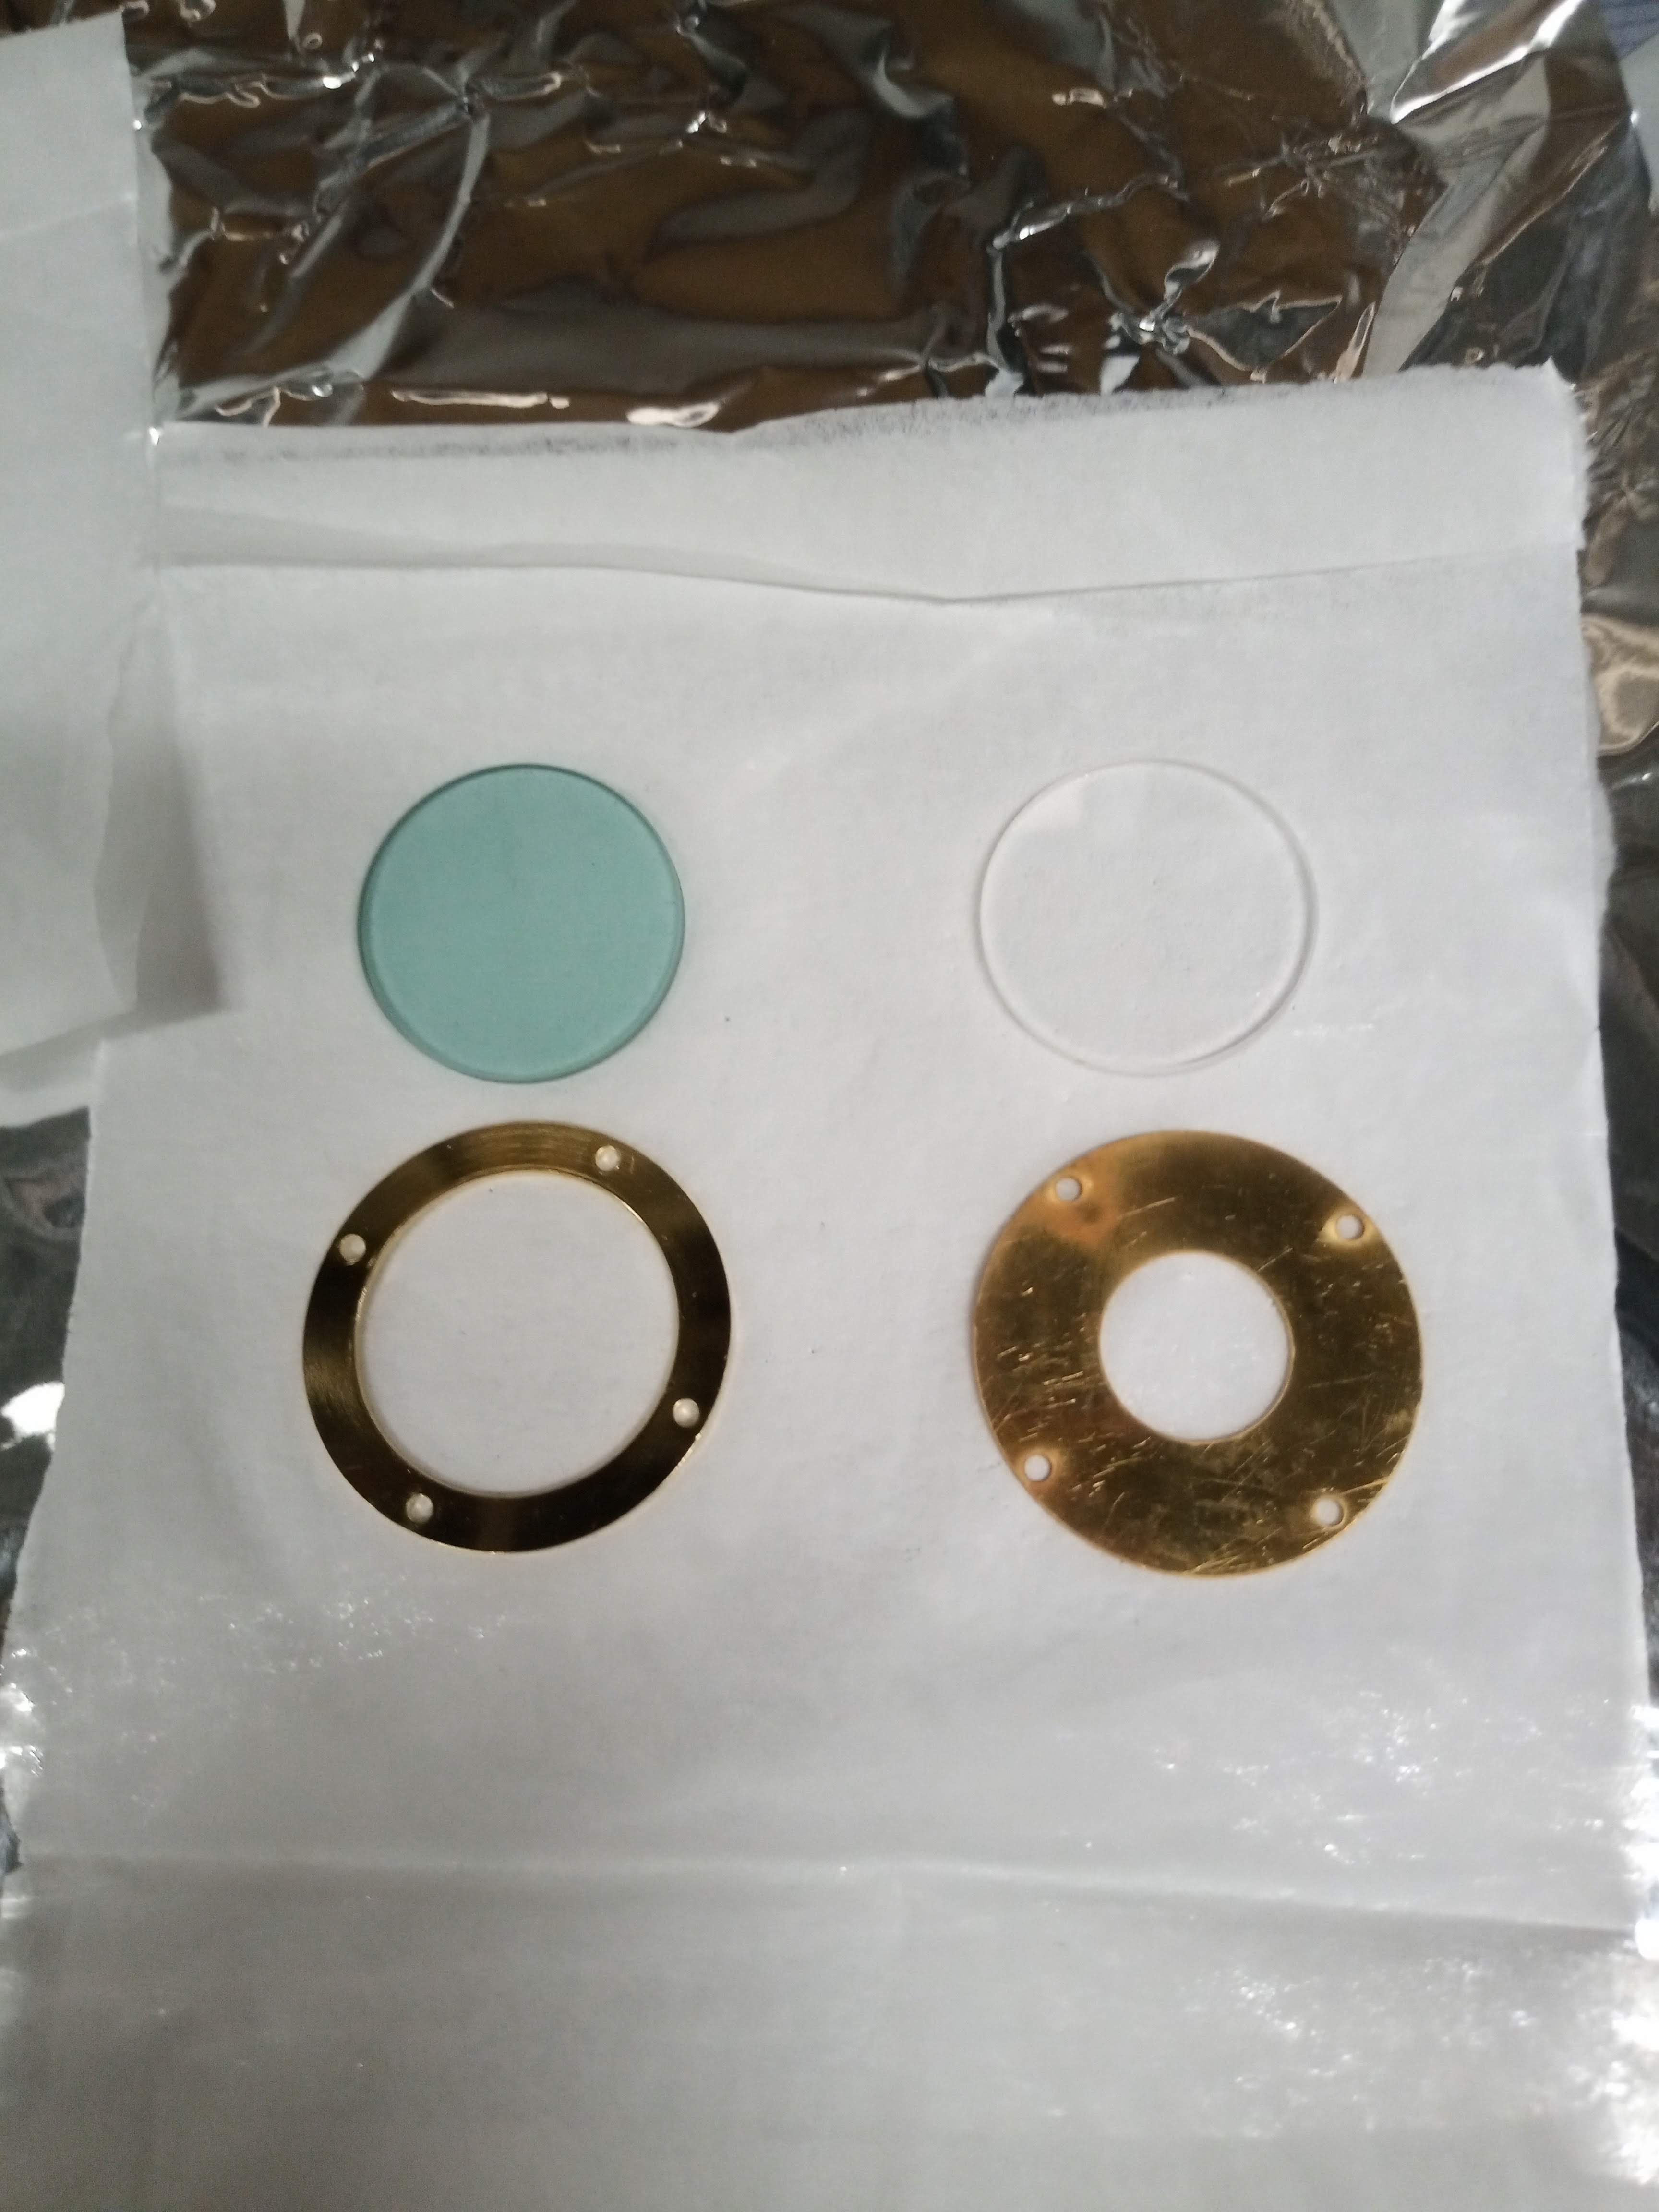
\includegraphics[width=\textwidth]{pictures/windows_filters.jpg}
        \captionsetup{width=0.9\textwidth}
        \caption{\emph{Left:} KG5 IR filter with \SI{20}{mm} opening cover. \emph{Right:} WG41050 bandpass filter with \SI{12}{mm} opening cover. }
    \end{subfigure}
    \hfill
    \begin{tabular}{c}
        \begin{subfigure}{.44\textwidth}
            \centering
            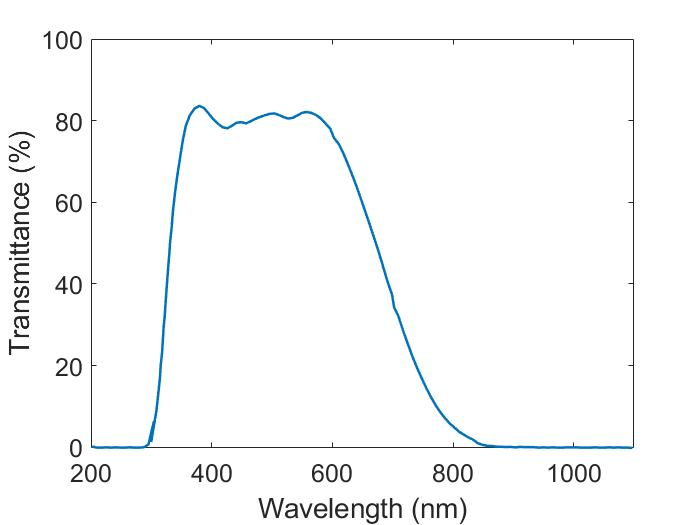
\includegraphics[width=\textwidth]{pictures/KG5_trans.jpg}
            \caption{KG5 transmission curve.}
        \end{subfigure}
      \\
        \begin{subfigure}{.44\textwidth}
            \centering
            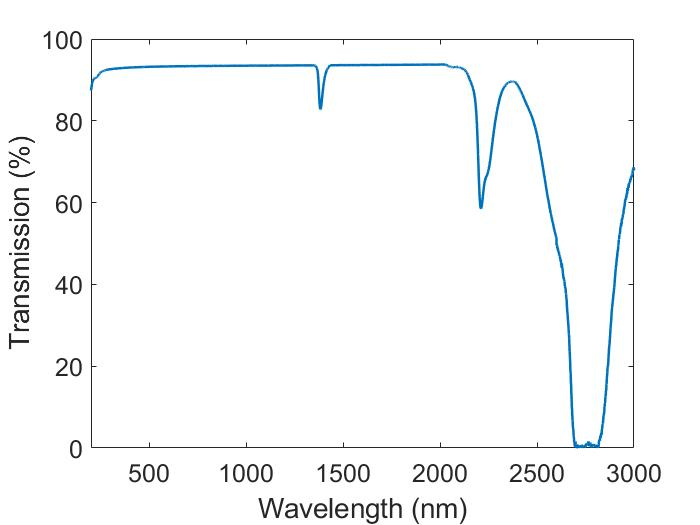
\includegraphics[width=\textwidth]{pictures/UVFS_trans.jpg}
            \caption{WG41050 transmission curve.}
        \end{subfigure}
    \end{tabular}
    
    \caption{Details of filters and windows. \textbf{(a)} IR and bandpass filters and respective windows. The transmission curves shown in \textbf{(b)} and \textbf{(c)}.}
    \label{fig:expsetup:windows}
\end{figure}


\subsection{Tip preparation}

In this thesis, a platinum/iridium (Pt/Ir) and a silver (Ag) tip was used. Below is a description of the tip preparation. The tips were then clamped into a custom Omicron tip holder and transferred into the microscope. 

The Pt/Ir tips were made by mechanically shearing a 0.38mm diameter wire. The Pt/Ir tip oxidizes relatively slowly and is relatively stiff, meaning it can be conditioned by poking into the metal substrates, resulting in a Ag or Au terminated Pt/Ir tip. 

\begin{figure} [h]
    \centering
    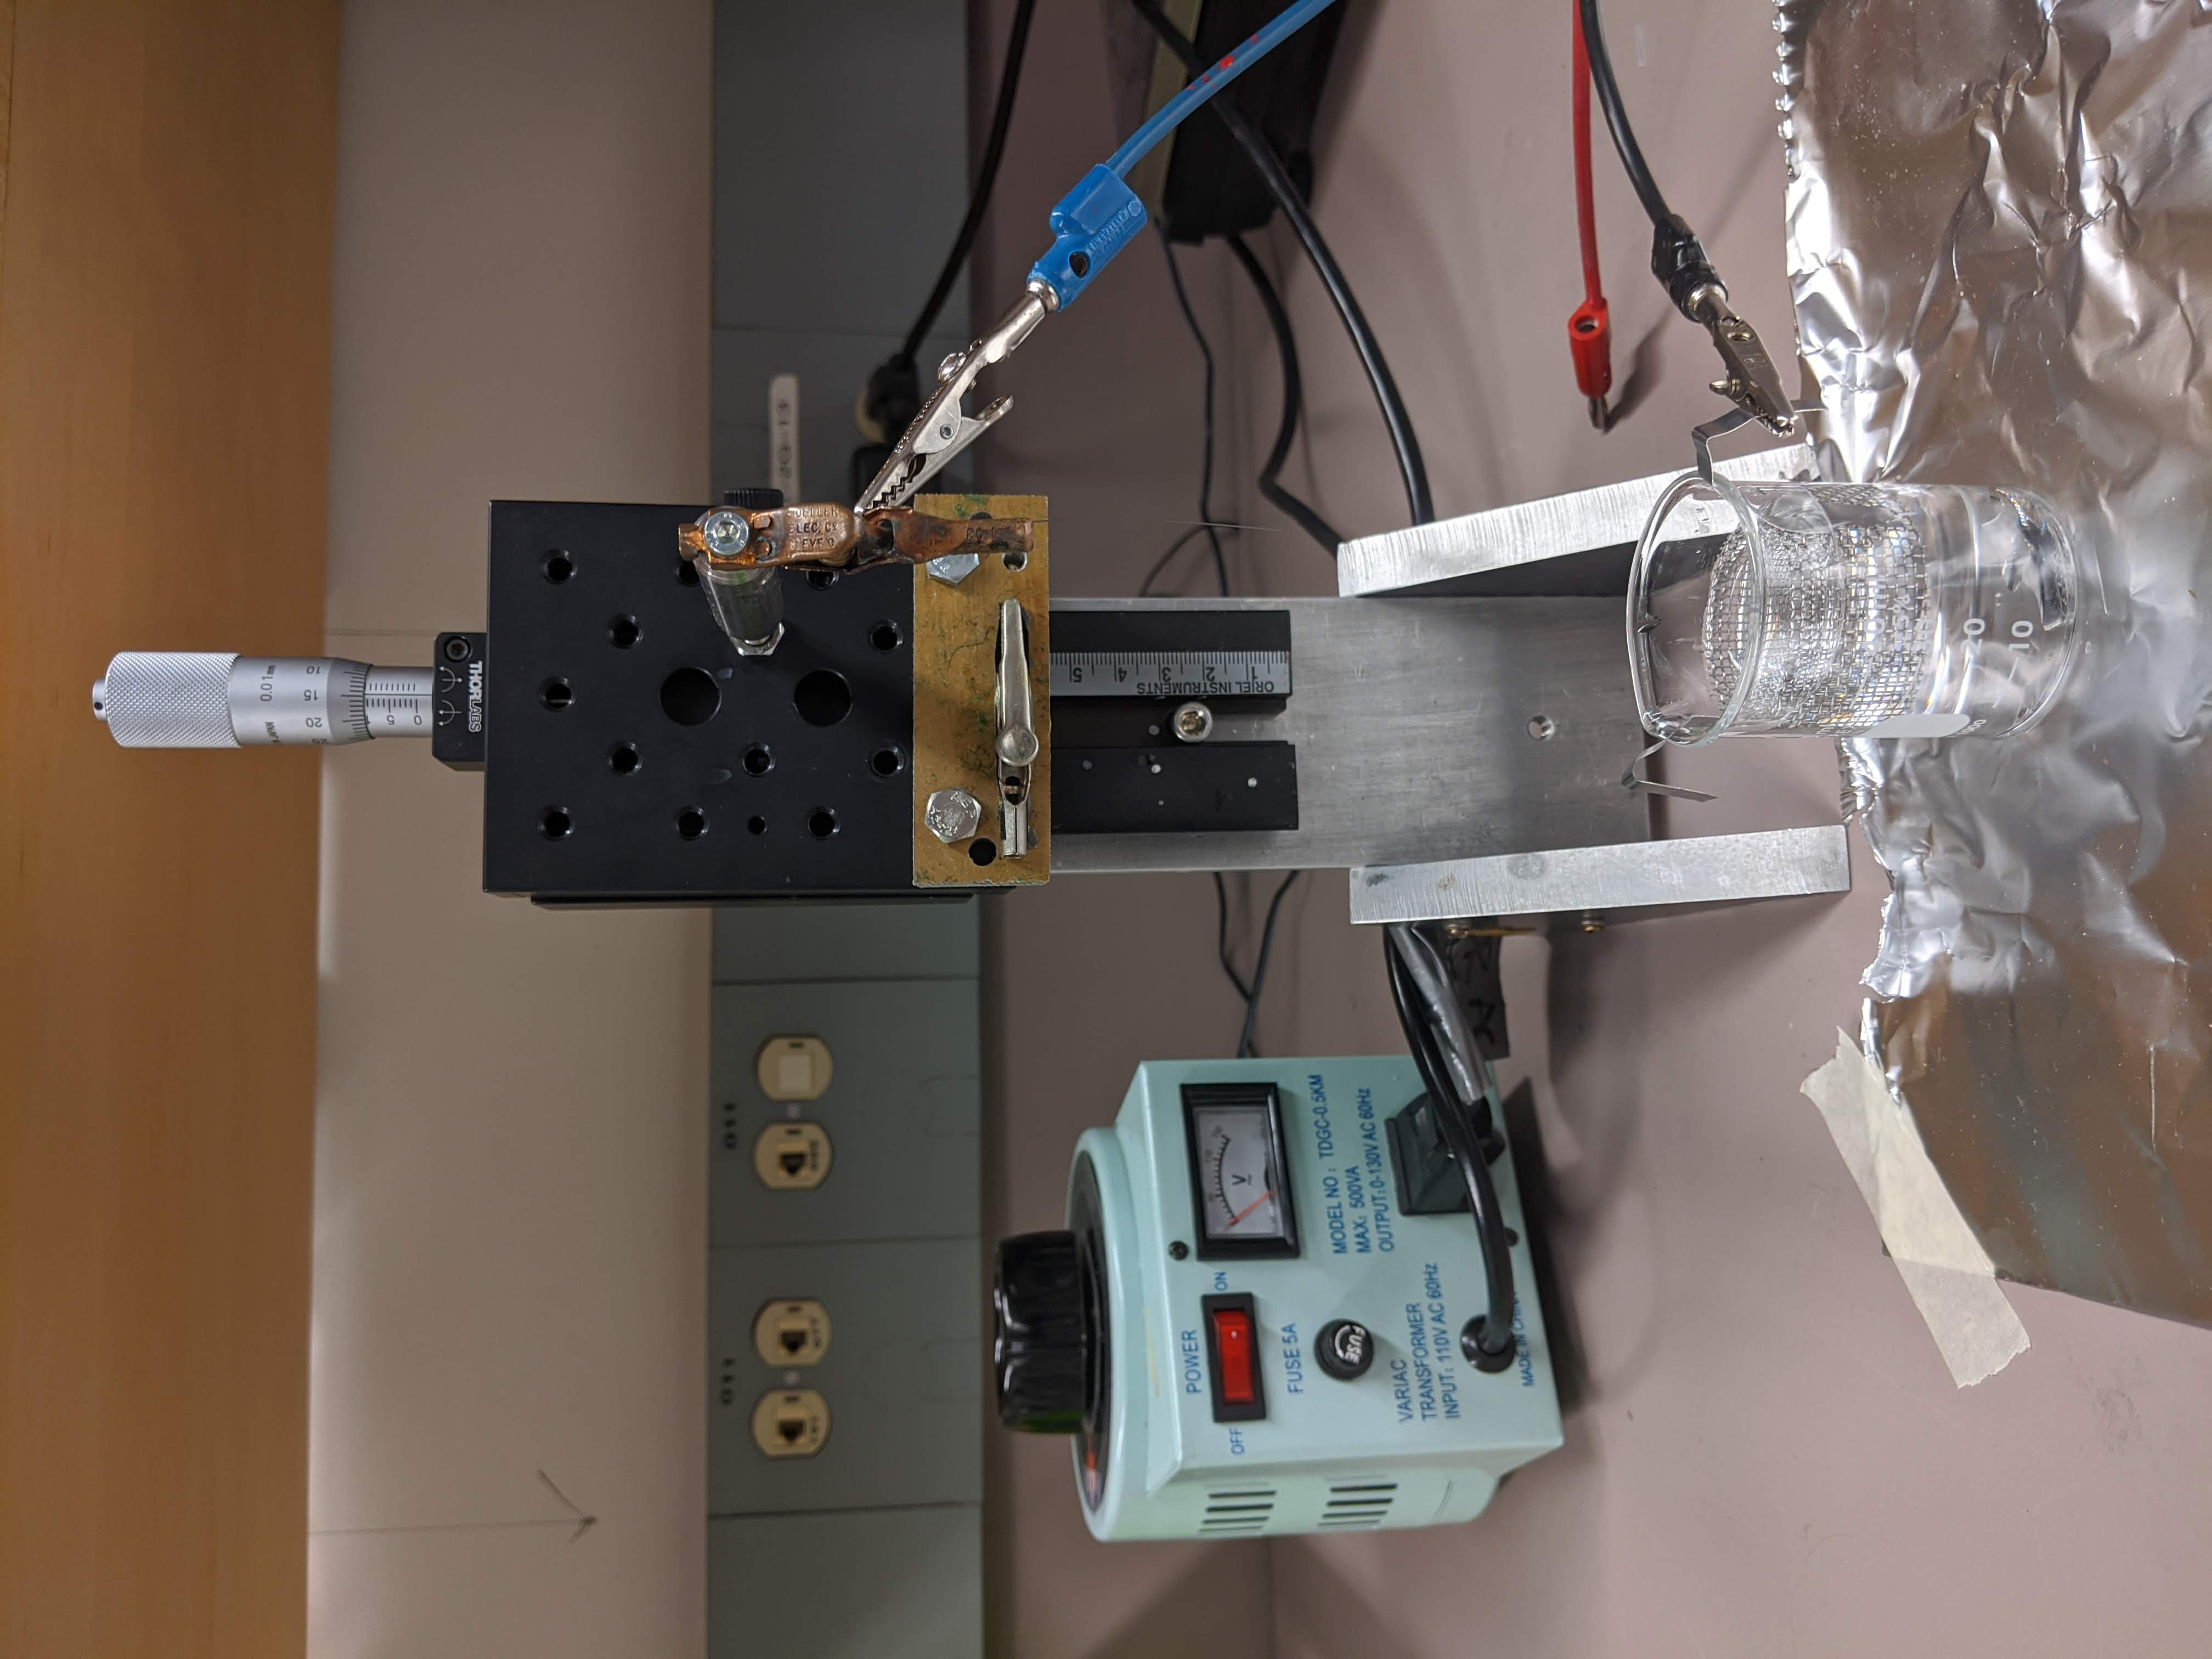
\includegraphics[width=3in,angle=-90]{pictures/etching.jpg}
    \caption{\FIXME{Caption for tip etching setup. Also include diagram for meniscus etching.}}
    \label{fig:expsetup:etching}
\end{figure}

Ag is a material with a low lossyness, making it optimal for \ac{STML}. Due to the importance of tip geometry in enhancing the luminescence signal, Ag tips were electrochemically etched, ensuring a well-defined and sharp tip shape. The procedures for Ag tip preparation are adapted from \citep{roussy2016coupling, zhang2011fabrication}. 

The etching setup is shown in \autoref{fig:expsetup:etching}. A 0.404mm diameter Ag wire was cleaned with acetone and isopropyl alcohol to give a clean etching surface. A teflon tubing covered the bottom $\sim$ \SI{3}{mm} of the wire to protect the region from chemical etching. The wire was then clamped and suspended in a solution of 50\% w/w citric acid in deionized water, with the meniscus about \SI{1.5}{mm} above the teflon protected region. A cylindrical mesh electrode was submerged into the solution with the wire in the centre to provide uniform etching on all sides of the wire. The wire was then etched using an alternating current voltage source at \SI{39}{V}, with the negative terminal connected to the wire, and the ground terminal connected to the mesh electrode. 

Etching typically took around \SI{30}{min}. Surface tension effects and preferential etching at the meniscus produces a sharp metallic tip from the submerged portion of the wire, which drops into the solution, breaking electrical contact with the negative terminal and ending etching processes (\autoref{fig:expsetup:etching}). The tip was removed from the solution with the sharp side facing away from the meniscus, as the surface tension can bend the tip. The teflon tubing was removed, and the tip was rinsed in deionized water, followed by acetone and isopropyl alcohol. The tip was then examined with an optical microscope to ensure the tip was macroscopically sharp, and possessed a shiny metallic surface (\autoref{fig:expsetup:image-plasmon}). With the tip exposed to air, the Ag is susceptible to oxidation which can quench luminescence signals. If the tip passed inspection, it was immediately mounted and placed under vacuum in the microscope. We found the most success with Ag tips that were exposed to air for no longer than \SI{20}{min}.

Due to the softness of Ag, it is extremely important that the tip does not crash into the surface. To prepare the tip for \ac{STML} experiments, the tip was repeatedly pulsed with voltages ranging from $5-\SI{10}{V}$ in order to remove residue and oxide from the tip. The shape of the tip was modified by piezo-controlled indentation into the metal substrate, ranging from 1$\SI{-10}{nm}$. With the optical setup aligned (discussed in the next section), the tip should demonstrate strong plasmonic emission at $\sim \SI{550}{nm}$ on Ag(111) when held at $V_b =\SI{3}{V}$ and $I_t = \SI{200}{pA}$ (\autoref{fig:expsetup:image-plasmon}).

\begin{figure} [h]
    \centering
    %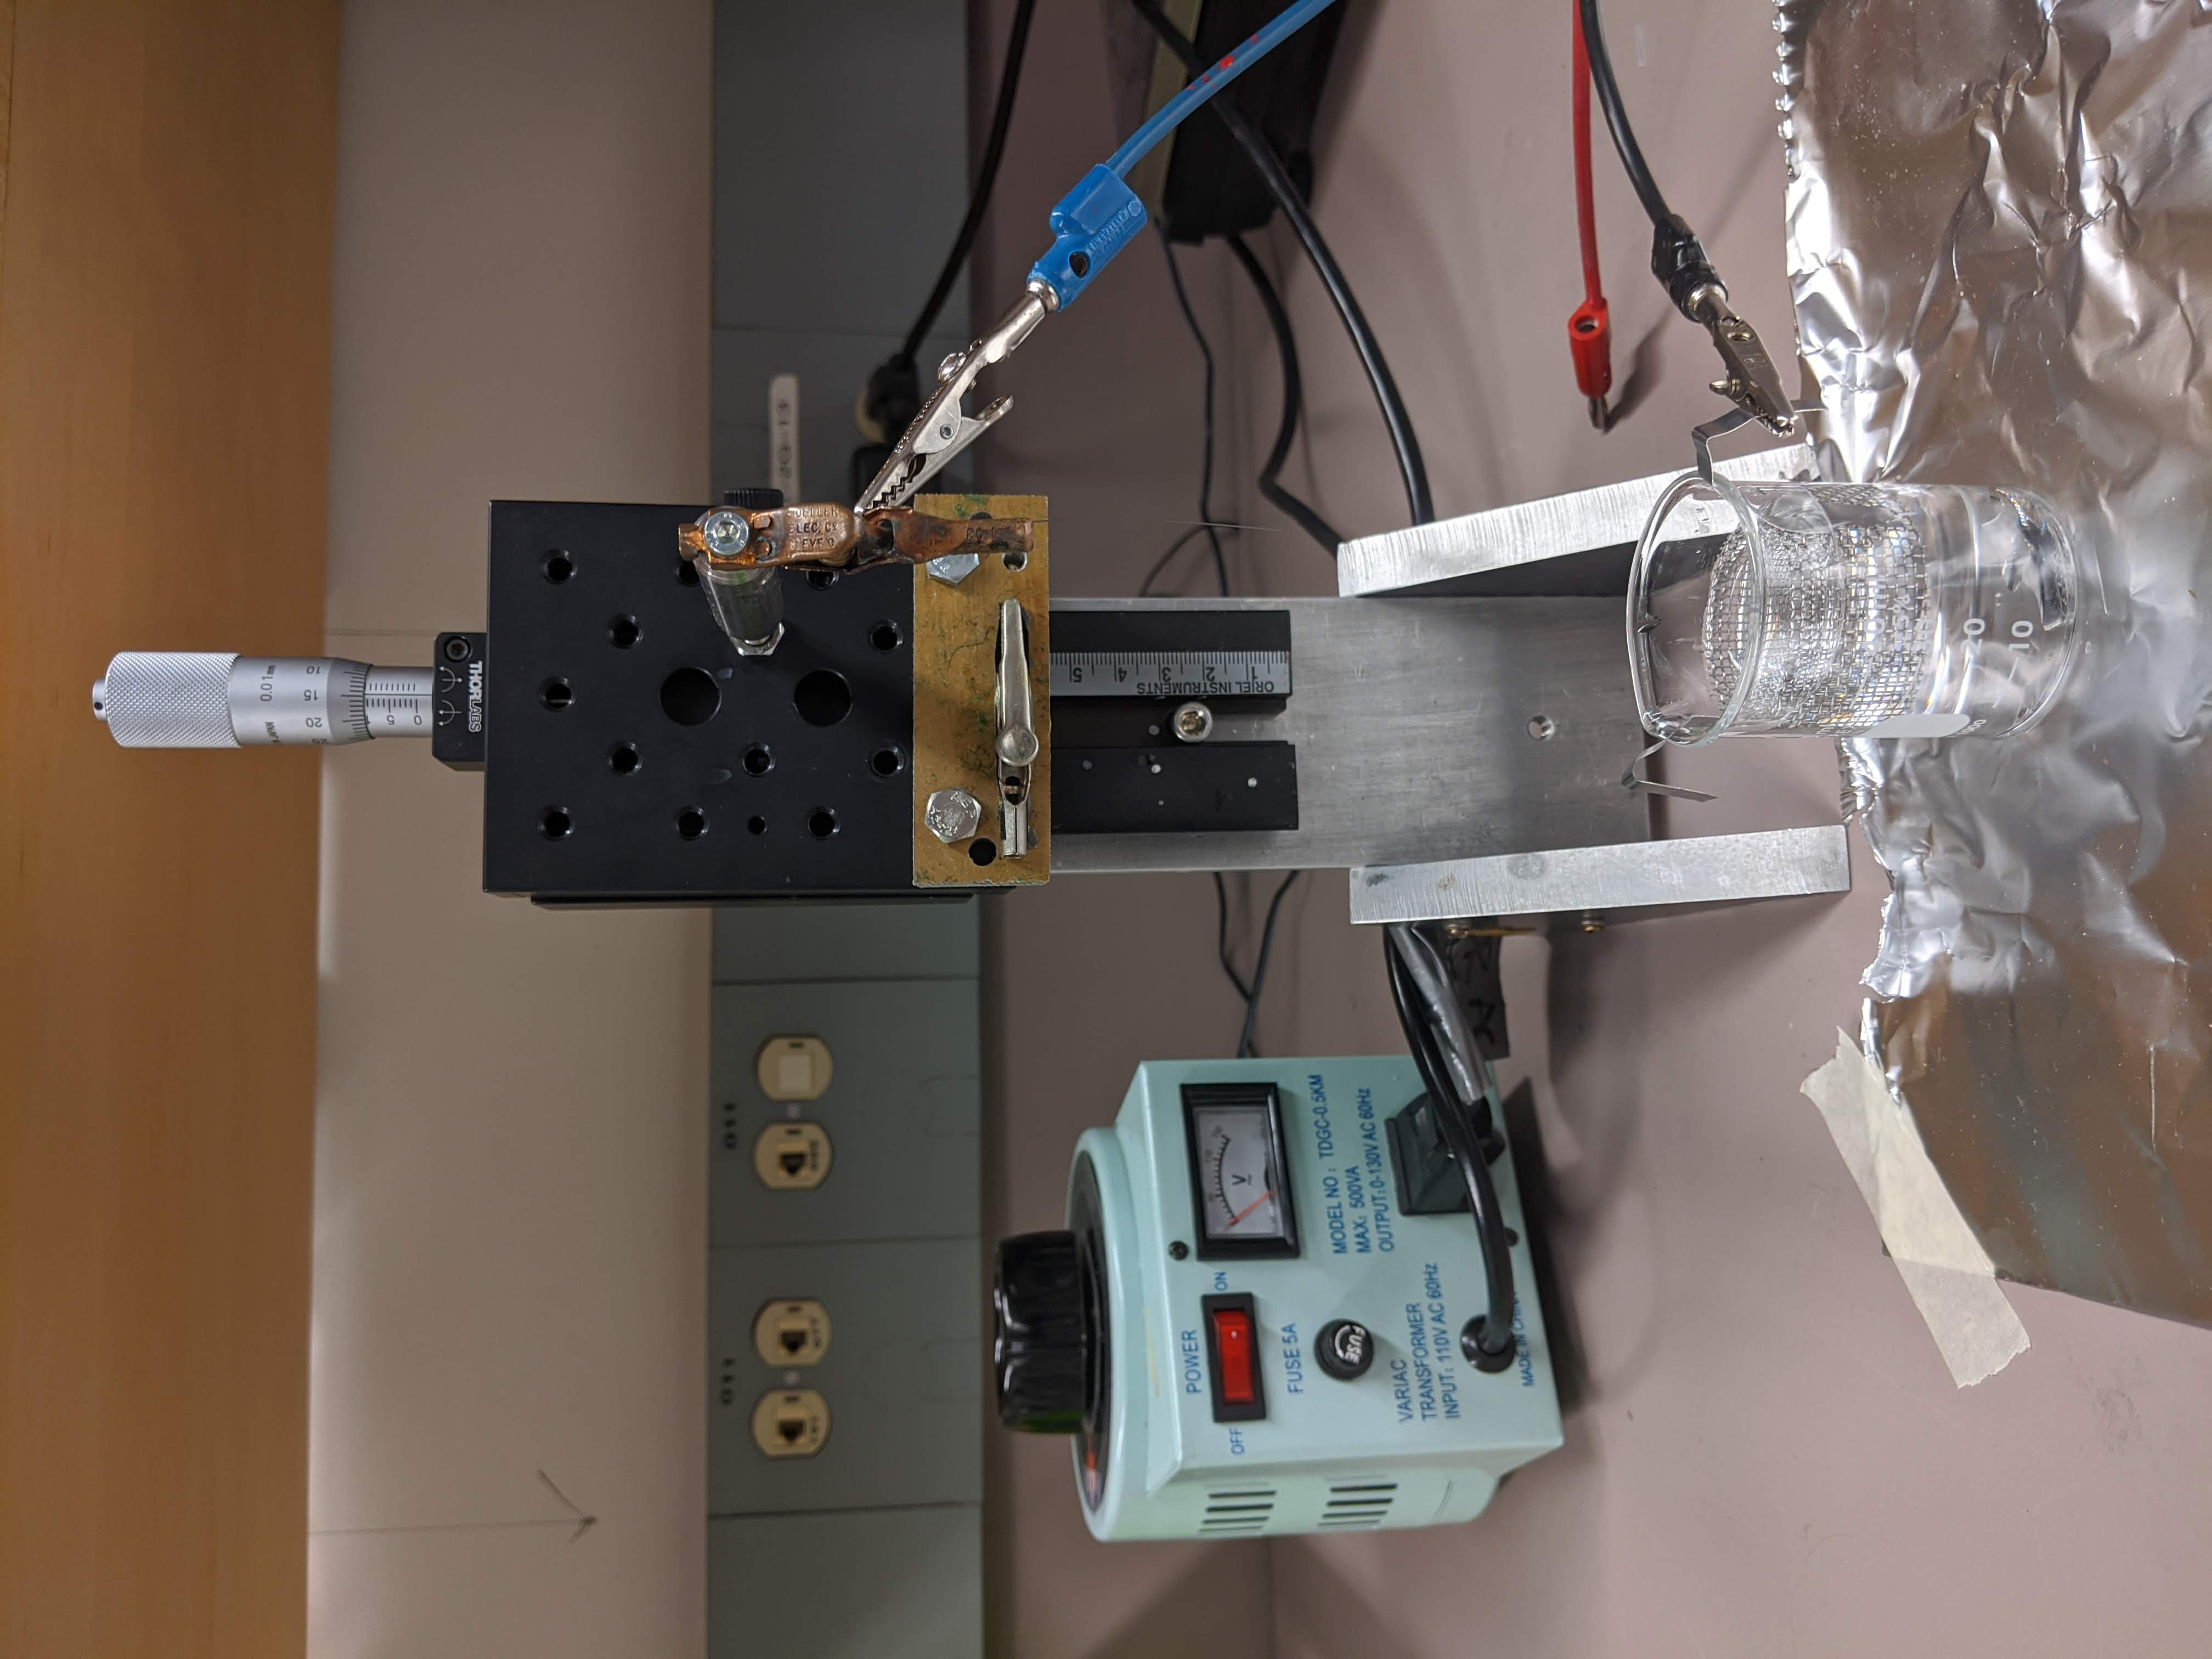
\includegraphics[width=3in,angle=-90]{pictures/etching.jpg}
    \caption{\FIXME{show some tips with plasmons (2-3).}}
    \label{fig:expsetup:image-plasmon}
\end{figure}




\subsection{External optical setup}

Light collected by the lens inside the \ac{SPM} head exited the \ac{LT} chamber through a viewport. The external optical setup is shown in \autoref{fig:expsetup:optics}. A mirror mounted on the viewport directed the photons toward an optical table installed on the microscope. On the optical table, another mirror directed the light into a lens mounted on a \textit{xyz} micrometer stage, focusing the light into a spectrometer. The spectrometer energetically resolved the incoming photons, and the signal was detected with a \ac{LN2} cooled \ac{CCD}. 

\begin{figure} [h]
    \centering
    %\includegraphics[width=3in]{file}
    \caption{\FIXME{Optical windows. With transmission curves.}}
    \label{fig:expsetup:optics}
\end{figure}

Before starting any experiment, the \ac{CCD} was calibrated for each spectrometer grating using a mountable Hg lamp. The provided software uses the characteristic emission peaks of Hg to correspond \ac{CCD} pixels to photon wavelength, with typical uncertainty values of $\pm$\SI{0.1}{nm}. In the presented work, two spectrometer gratings were used, with grating densities 300 gratings (gr)/mm and 600 gr/mm.\footnote{Some signal may be lost due to the imperfect reflectivity of the gratings. Efficiencies of the gratings at the regions of interest are around $70 - 80 \%$ \citep{princetongratings}} Higher grating density allows for higher resolution at the expense of spectral range. Once calibrated, all light sources in the room were covered or turned off and a background spectrum was taken. This background spectrum is subtracted from all experimental data, and accounts for thermal noise and stray light in the room.

The optical setup was then aligned to ensure that emission from the tip-sample junction entered the spectrometer. To begin, the lens on the optical table was removed, and the tip was coarse approached to the sample. The face of the spectrometer was illuminated such that a shadow of the slit could be seen on the surface of the metallic substrate. The shadow of the slit and the tip-sample junction were aligned, either by moving the tip or changing the angle of the two mirrors. With the tip-sample junction and spectrometer slit aligned, the lens can be mounted onto the micrometer stage. Shining light in through the camera port, the light reflected off the tip-sample junction can be focused into the spectrometer slit by adjusting the position of the lens.

All measurements were done with the largest slit opening (\SI{3}{mm}) to maximize the amount of light entering the spectrometer. This comes at a cost: spectral features that are sharper than a \ac{FWHM} of \SI{3}{nm} (for the 300 gr/mm) or \SI{1}{nm} (for the 600 gr/mm) are broadened and not resolved \citep{princetonslit}. 



\section{Sample preparation}

Sample preparation involves cleaning the substrate, depositing the \ch{NaCl} film, and depositing the molecules. In this thesis, five different organic semiconducting molecules were studied, each with different deposition parameters. All sample preparation procedures will be discussed in detail.

\subsection*{Ag(111) substrate}

A top hat silver crystal with (111) termination is the primary substrate used for experiments. The crystal surface is cleaned by sputtering for \SI{20}{\minute} using ionized \ch{Ar} gas, with ionizing potential $\sim \SI{1}{kV}$ and preparation chamber pressures at $P_{prep} \approx 3 \times 10^{-6}$ mbar. The substrate is then annealed using an e-beam heater at $T_{sub} = \SI{420}{\celsius}$ for another \SI{20}{\minute}. This is repeated 2--3 times depending on the status of the crystal surface.

A typical scan of a clean Ag(111) surface is seen in \autoref{fig:expsetup:Ag111}. When scanned with a sharp metallic tip, step heights are typically $\sim\SI{2}{\angstrom}$, and the \ac{STS} point spectra has a ``kink" at \SI{-67}{mV}. This corresponds to a step in the density of states, approximated by $dI/dV$, which is a result of the surface state of Ag(111) \citep{hovel2001modification}.

\begin{figure} [h]
    \centering
    %\includegraphics[width=3in]{file}
    \caption{\FIXME{Ag(111) with few defects., also show the STS/dIdV.}}
    \label{fig:expsetup:Ag111}
\end{figure}


\subsection*{Au(111) on Mica substrate}

As an alternate substrate, a thin film of (111) terminated gold on mica was used. The cleaning is similar to the procedures for Ag(111), but with sputtering potential $\sim \SI{0.75}{kV}$, and annealing temperature $T_{sub} = \SI{345}{\celsius}$.

An \ac{STM} image of the Au(111) thin film (\autoref{fig:expsetup:Au111}) shows a herringbone structure as a result of the reconstruction of the surface into regions of face centred cubic and hexagonal close packed atomic arrangements \FIXME{citation}. Step heights on the surface are $\sim \SI{2}{\angstrom}$. The \ac{STS} spectra shows the onset of the surface state to be at around $\SI{-450}{mV}$.

\begin{figure} [h]
    \centering
    %\includegraphics[width=3in]{file}
    \caption{\FIXME{Ag(111) with few defects., also show the STS/dIdV.}}
    \label{fig:expsetup:Au111}
\end{figure}


\subsection*{NaCl deposition}

Layers of \ch{NaCl} were deposited onto the metallic substrates for all experiments discussed in this thesis. The film grows with (100) surface. This insulating film partially decouples the molecule from the metallic substrate, while still allowing for tunnelling between the tip and sample \citep{repp2005molecules}. The decoupling is also necessary for \ac{STML} experiments, as emission from excitons in the molecule are quenched by electronic pathways between the molecule and the metal substrate.

NaCl was thermally deposited using a homebuilt Knudsen cell. The thickness of the film can be controlled by deposition temperature, time, and substrate temperature. With the substrate held at $T_{sub} = \SI{100}{\celsius}$, NaCl was deposited for \SI{12}{\minute} with deposition temperature at approximately \SI{550}{\celsius}. 

\begin{figure} [h]
    \centering
    %\includegraphics[width=3in]{file}
    \caption{\FIXME{Bi and tri layer of nacl on ag111}}
    \label{fig:expsetup:2-3NaCl}
\end{figure}

\ac{STM} of bilayer and trilayer (2-\acf{ML} and 3\ac{ML}) NaCl on Ag(111) is shown in \autoref{fig:expsetup:2-3NaCl}, seen as rectangular terraces. The step height of 2\ac{ML} NaCl is around \SI{3}{\angstrom}, while 3\ac{ML} is at \SI{4.5}{\angstrom}. Experiments were carried out on the bilayer (2\ac{ML}) for better molecule and tip stability.

The presence of the NaCl layers shifts the onset of the surface state of the metallic substrates (\autoref{fig:expsetup:NaClstate}). This signature in the \ac{STS} spectra is useful for determining whether a surface is metallic or insulating NaCl.

\begin{figure} [h]
    \centering
    %\includegraphics[width=3in]{file}
    \caption{\FIXME{NaCl state on ag and au}}
    \label{fig:expsetup:NaClstate}
\end{figure}

\subsection*{Molecule deposition}

Five different organic semiconducting molecules were used in our experiments (\autoref{fig:expsetup:molecules}). All molecules were deposited on a cold sample in the \ac{LT} chamber, with substrate temperature between \SI{4.3}{K} and \SI{4.5}{K}. The deposition parameters are summarized in \autoref{tab:expsetup:mol-dep}. 

\begin{figure} [h]
    \centering
    %\includegraphics[width=3in]{file}
    \caption{\FIXME{Chemical structures of all molecules}}
    \label{fig:expsetup:molecules}
\end{figure}

The \ac{HMAT} derivative molecules were synthesized by C. Tonge in the Hudson group in the chemistry department of \ac{UBC}. To obtain the deposition temperature for these molecules, thermogravimetric analysis was performed to give an approximate temperature at which the molecule begins to degrade. The molecules were then deposited onto the sample at approximately \SI{50}{\celsius} below the degradation temperature, and the sample scanned for presence of the molecules. The deposition temperature was ramped up in \SI{5}{\celsius} increments until the molecule was found on the surface.

\begin{table} [h]
\begin{center}
    \begin{tabular}{|c|c|c|} 
    \hline
        Molecule  &  \begin{tabular}[x]{@{}c@{}}Deposition\\temperature (\SI{}{\celsius})\end{tabular}   &  Time \\
        \hline
         PTCDA    &     325   & $\sim \SI{30}{s} $  \\
          ZnPc  &      370  & $\sim \SI{30}{s}$   \\
     \ch{F8ZnPc} &     370 & $\sim \SI{30}{s}$ \\
        HMAT-O   &    160  &    \SI{5}{\minute}\\
        HMAT-TZ  &    330   &  \SI{5}{\minute}\\
        HMAT-HZ  &    330  & \SI{10}{\minute}  \\
        \hline
    \end{tabular}
    \caption{Deposition times presented vary depending on the desired coverage. The times listed are for sparse coverages. The deposition may be repeated multiple times until coverage is sufficient. }
    \label{tab:expsetup:mol-dep}
    \end{center}
\end{table}


Unfortunately, the \ac{HMAT} derivatives were not stable at the sublimation temperature. Repeated degassing to remove impurities in the crucible resulted in continued deposition of molecular fragments. In order to preserve the integrity of the molecules, the deposition temperature was lowered, and the deposition time increased to the order of minutes.













\section{Simulation methods}

\Acf{DFT} calculations were performed for the molecules, giving the molecular orbitals and energy levels of the isolated molecules. The results can be qualitatively compared to the experimental results. First, the chemical structures were drawn with the \textit{Avogadro} software \citep{hanwell2012avogadro}, which generated a file with the \ac{3D} coordinates of the atoms. As organic molecules can be flexible, different conformations were generated using the knowledge-based \ac{ETKDG} algorithm \citep{riniker2015better} built into the Python package \textit{RDKit} \citep{rdkit}. The \ac{UFF} \citep{rappe1992uff} was used to calculate the energy of the conformations, and the conformation with the lowest energy was selected for \ac{DFT} calculations. Due to the many aromatic rings in the molecules we studied, the possible conformations were limited to planar structures, comparable to the planar configuration of the molecules on our metallic substrate.

Molecular orbitals and energy levels of free molecules were calculated using \ac{DFT} \emph{Gaussian 16} software package \citep{frisch2016gaussian}. The \ac{B3LYP} functional \citep{lee1988development,becke1993becke} and the 6-31G(d) \citep{frisch1984self} basis set was used for all calculations. A geometry optimization was performed on the conformer generated from molecular dynamics until the average force on all atoms were below $3\times 10^{-4}$ Ha/$r_{bohr}$. Finally, electronic structures of the fully relaxed molecules were calculated. The molecular orbitals were plotted with \textit{Avogadro}, while the energy levels were extracted with the \textit{Multiwfn} software \citep{lu2012multiwfn}. 

It is important to reiterate that the \ac{DFT} results can only be qualitatively compared with the experimental results. The \ac{DFT} calculations on the isolated molecules do not account for the interactions between the substrate and the molecule such as hybridization or by Van der Waals forces. Additionally, geometrical changes to the molecule occur when they are adsorpted onto a surface, and a variety of stable conformations are possible.

%%%%%


% opv molecules
%% The following is a directive for TeXShop to indicate the main file
%%!TEX root = diss.tex

\chapter{Conventional Organic Semiconducting Molecules}
\label{ch:opv}

%%%%%


% oled moelcules
%% The following is a directive for TeXShop to indicate the main file
%%!TEX root = diss.tex

\chapter{Engineering Organic Molecular Energy Levels}
\label{ch:oled}

% importance of engineering energy levels (optical gap, colour, applications in biomedical imaging?)
% can be done by using functional groups
% can examine the single molecule effects of functionalization 

The energy levels of organic semiconducting molecules determines the electronic and optical properties of the molecule. For different applications, there are different optimal energy level alignments. Through variation in the design of organic molecules, possible through organic synthesis techniques, the energy levels of the organic semiconductor can be engineered. This is realised through the addition of functional groups to an organic molecule or polymer \citep{schwarze2016band, VanMullekom2001}. In particular, this chapter will discuss the functionalization of \ac{HMAT} with various acceptor complexes, with \ac{HMAT} acting as the donor, and the resulting molecular orbitals and their energy levels. I will also discuss the attempts of \ac{STML} experiments on these \ac{HMAT} derivative molecules.




\section{Introduction to HMAT}

% talk about the HMAT molecule, where it came from
% why we are interested?
% possible functionalization of molecules

\Acf{HMAT} is a highly stable and planar molecule with interesting optoelectronic properties. With a theoretical HOMO-LUMO gap of \SI{4.45}{eV}, \ac{HMAT} is a good electron donor molecule and a deep blue-violet fluorophore \cite{Tonge2020} (\autoref{fig:oled:dft-hmat}). With a rigid planar structure, electrons in \ac{HMAT} have enhanced $\pi$-conjugation, giving it a high quantum photoluminescent efficiency, along with a high photon absorption cross-section \citep{Makarov2012}. Additionally, functionalized \ac{HMAT} derivatives have demonstrated optical effects such as thermally activated triplet exicton formation \citep{Chen2017}, and two-photon excited fluorescence \citep{Fang2012,Paisley2020}, making these molecules candidates for \ac{OLED} and biological imaging applications. 

\begin{figure} [h]
    \centering
    %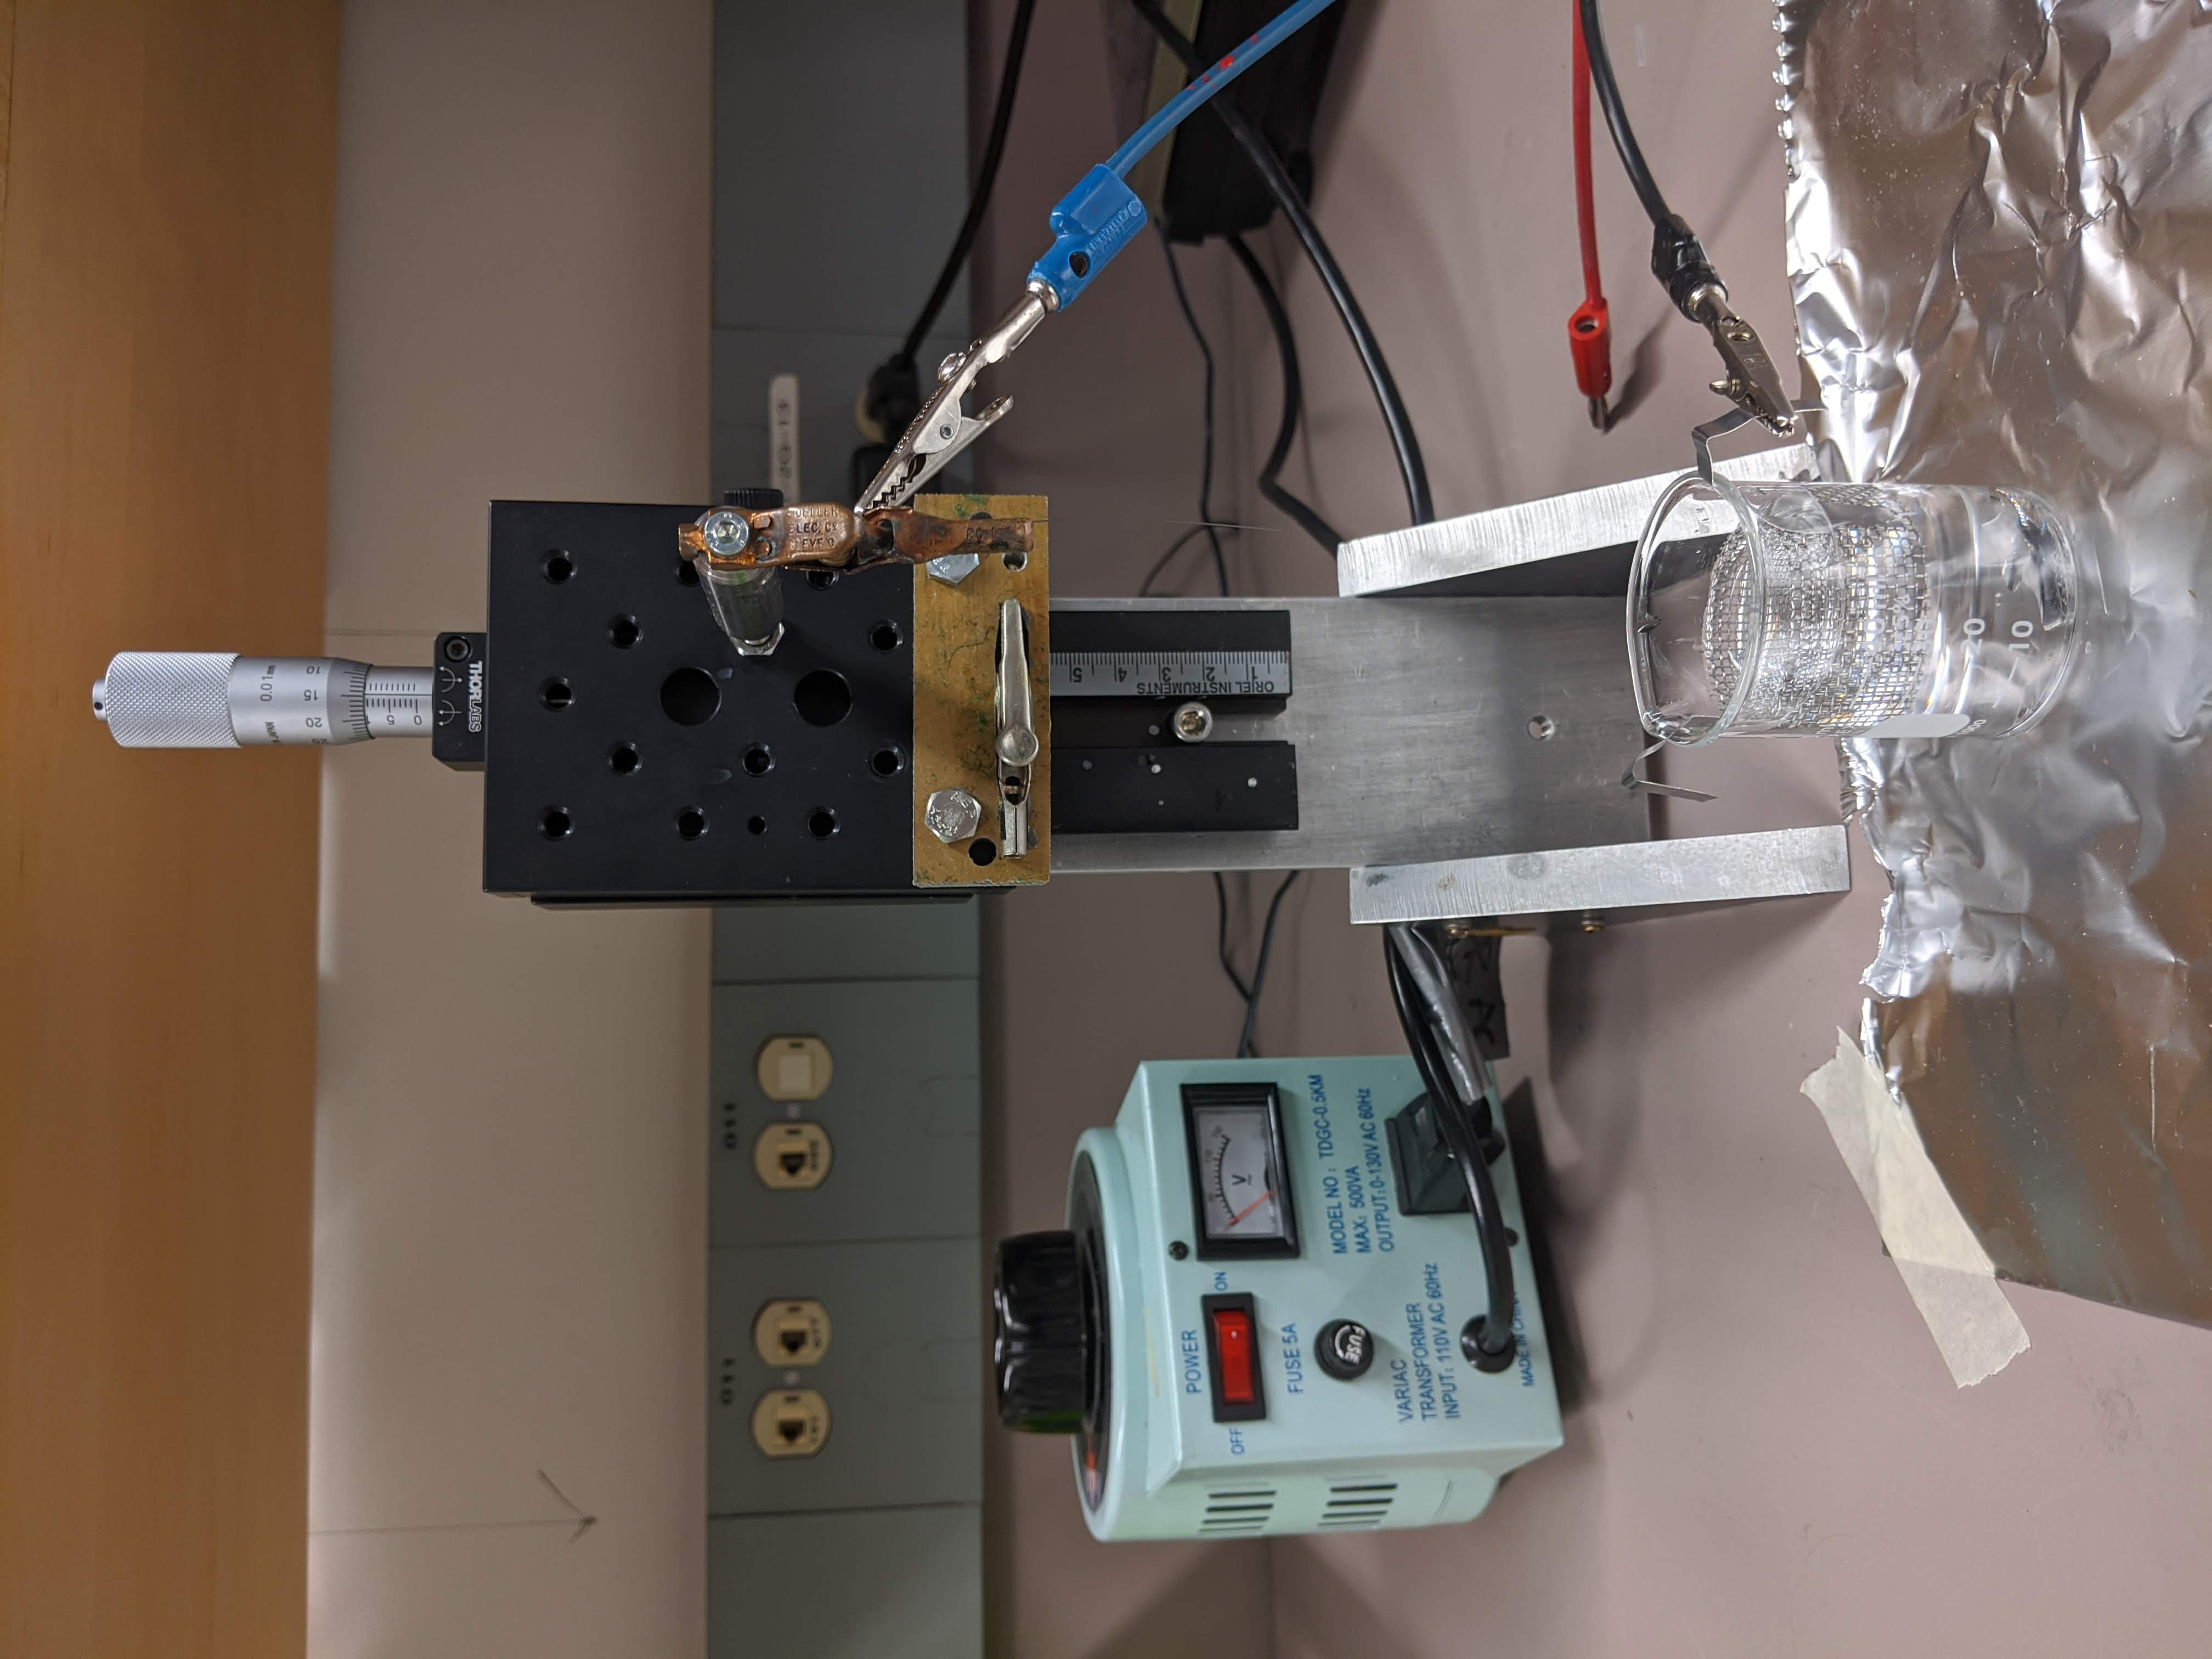
\includegraphics[width=3in,angle=-90]{pictures/etching.jpg}
    \caption{\FIXME{DFT of HMAT alone}}
    \label{fig:oled:dft-hmat}
\end{figure}

Being relatively difficult to synthesize, \ac{HMAT} and the functionalized derivatives were not available commercially and was provided by our collaborators in the chemistry department at \ac{UBC}. We examined three different \ac{HMAT} derivative molecules: \ac{HMAT-O}, \ac{HMAT-TZ}, and \ac{HMAT-HZ}. The chemical structure of each is shown in \autoref{fig:oled:hmat-derivatives}. All prior studies on \ac{HMAT} and its functionalized derivatives were in chemical ensembles with conventional analytical techniques. With \ac{SPM}, for each functional group, we can visualize the sub-molecular spatial distribution of the orbitals, and measure the energy levels of the single molecule. 

% are relatively difficult to synthesize molecules, that are not commercially available. Provided by our collaborators in the chemistry department at UBC, they have only been examined using conventional analytical chemistry techniques as a chemical ensemble. Here, we present a submolecular study of molecules that are derived from HMAT, a highly stable molecule with a large HOMO-LUMO gap capable of efficiently emitting ultraviolet light. By adding functional groups of increasing electronegativity, the HOMO-LUMO gap and the colour of emission can be tuned. 


\begin{figure} [h]
    \centering
    %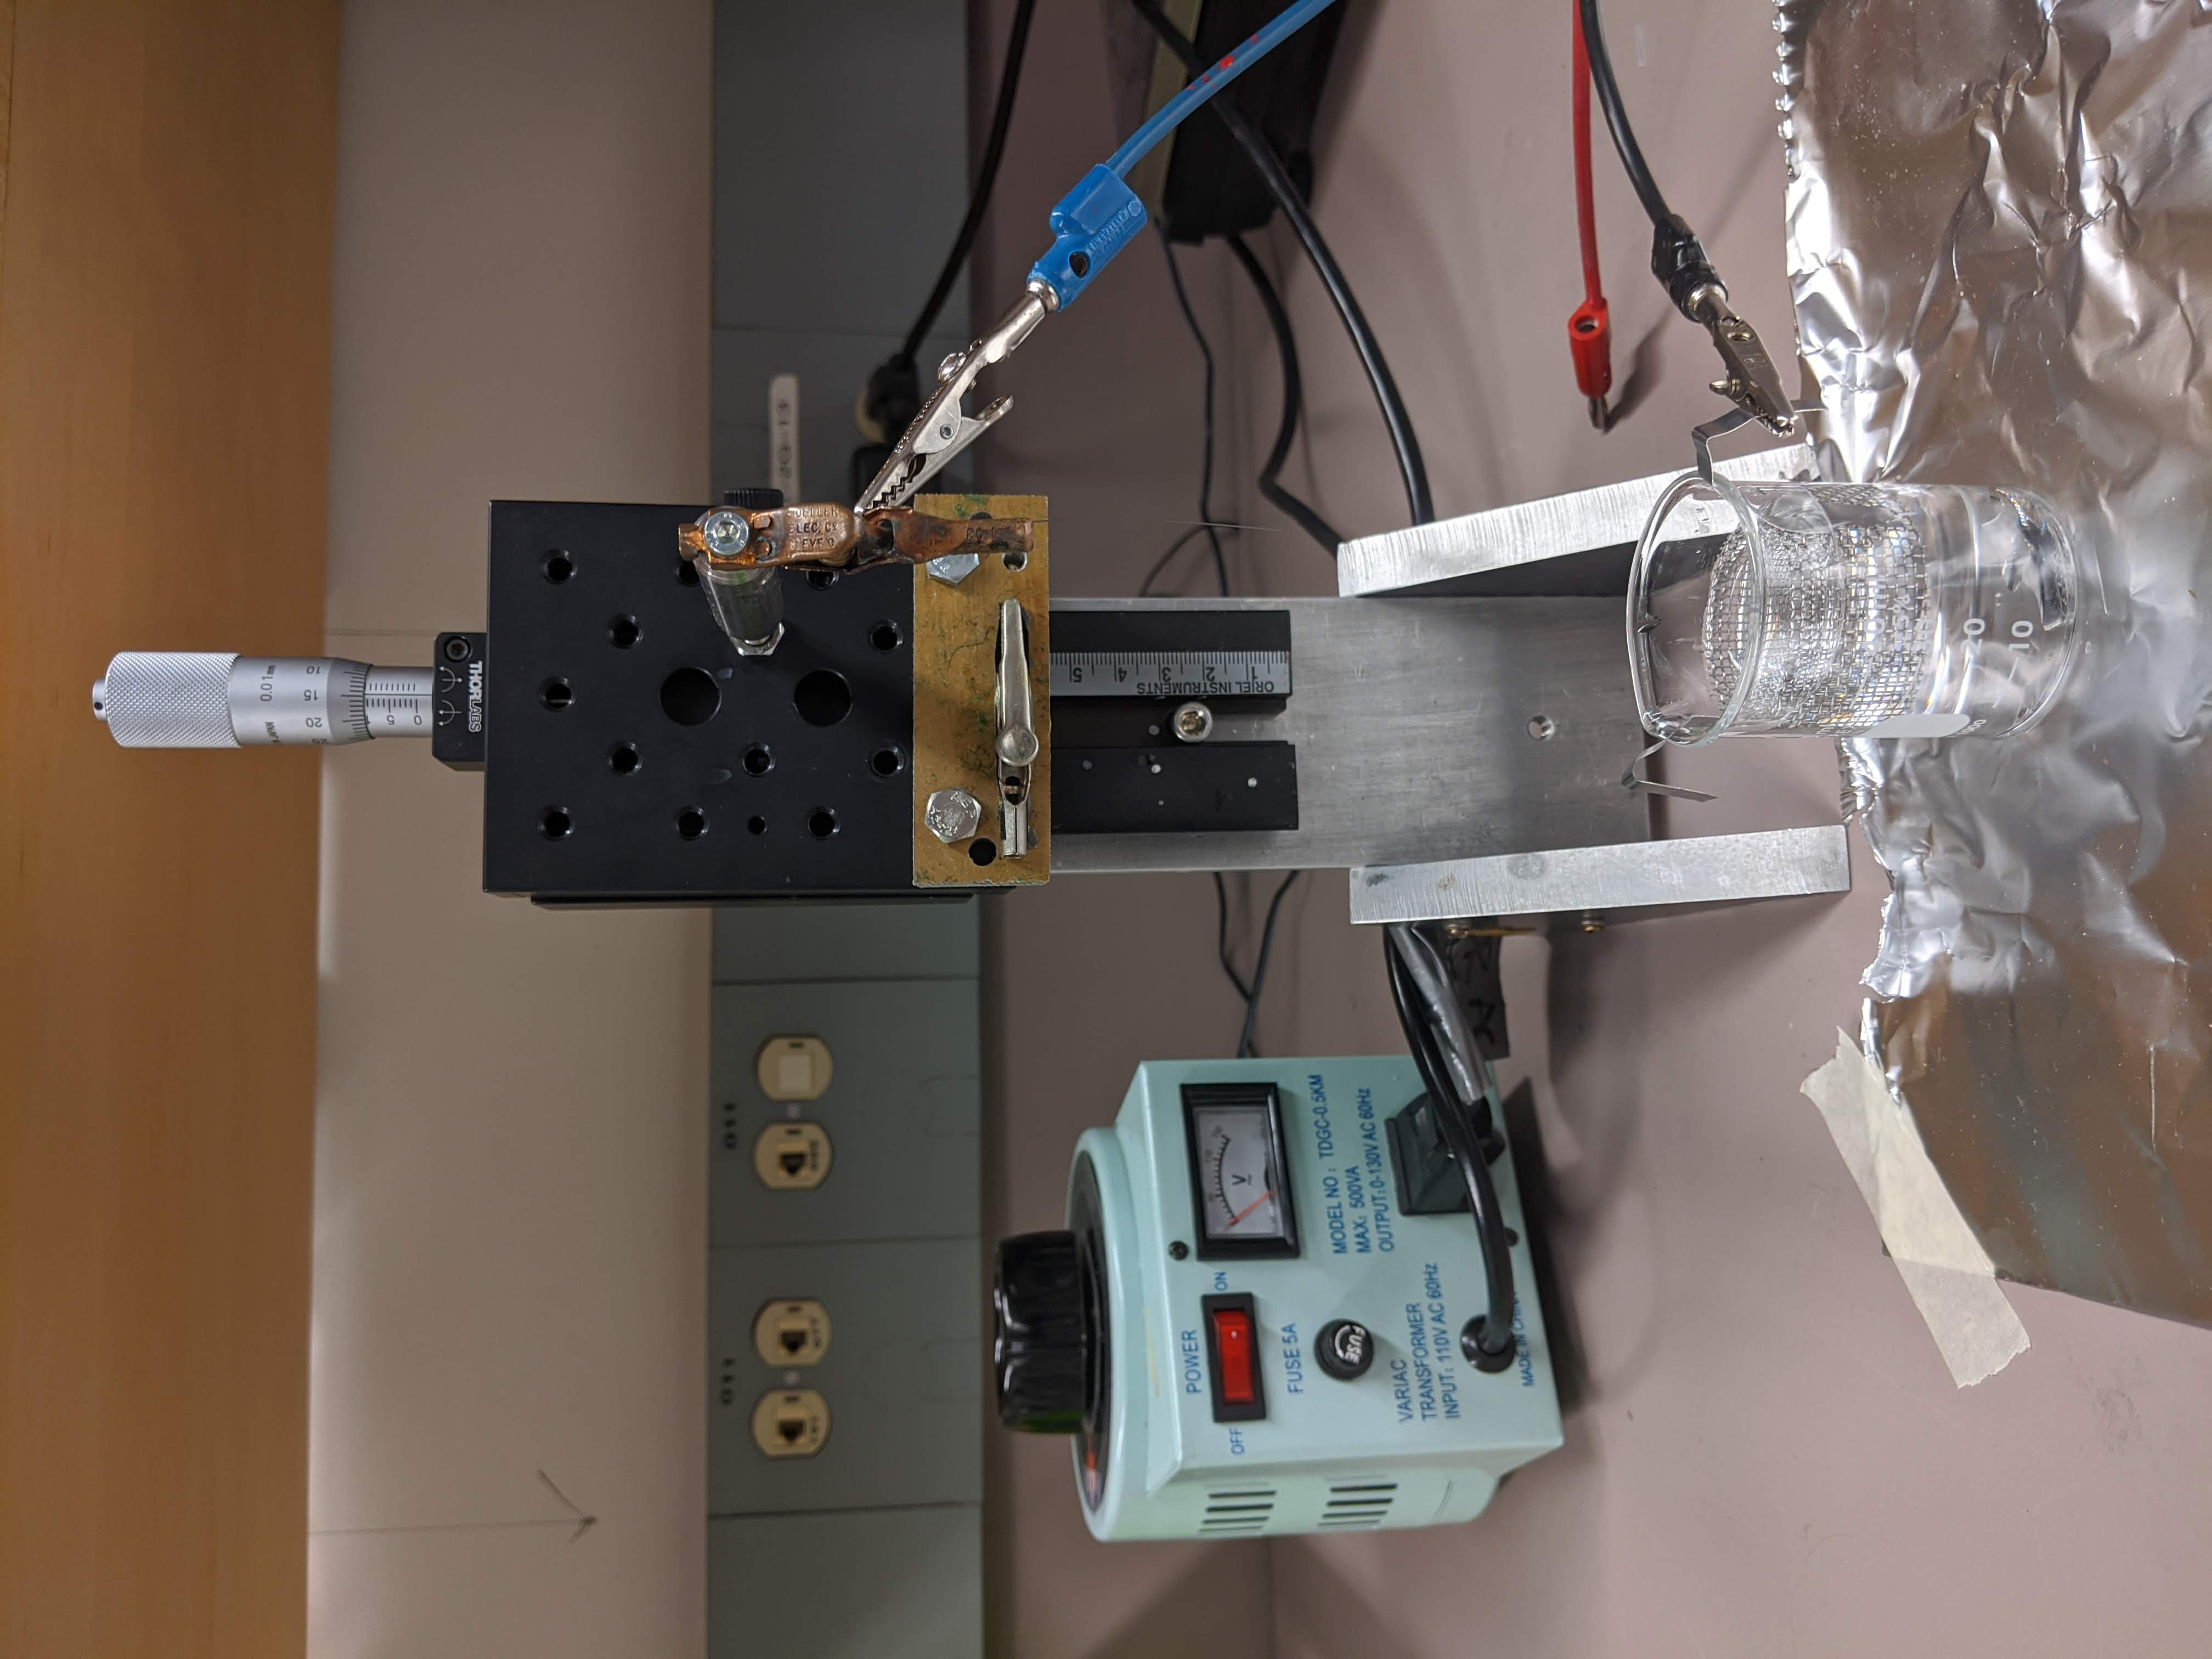
\includegraphics[width=3in,angle=-90]{pictures/etching.jpg}
    \caption{\FIXME{chemical structures of hmat and derivatives}}
    \label{fig:oled:hmat-derivatives}
\end{figure}




\section{{STM}/{STS} study of HMAT derivatives}

The molecules were deposited onto the bare Ag(111) surface, and probed with a Pt/Ir tip dipped in silver. While the \ac{HMAT} molecule is highly stable, the attached functional groups were fragmented at high deposition temperatures. Large area \ac{STM} scans showed an abundance of fragments on the surface for each molecule deposition, even after repeated degassing (\autoref{fig:oled:hmat-frag}). 

\begin{figure} [h]
    \centering
    %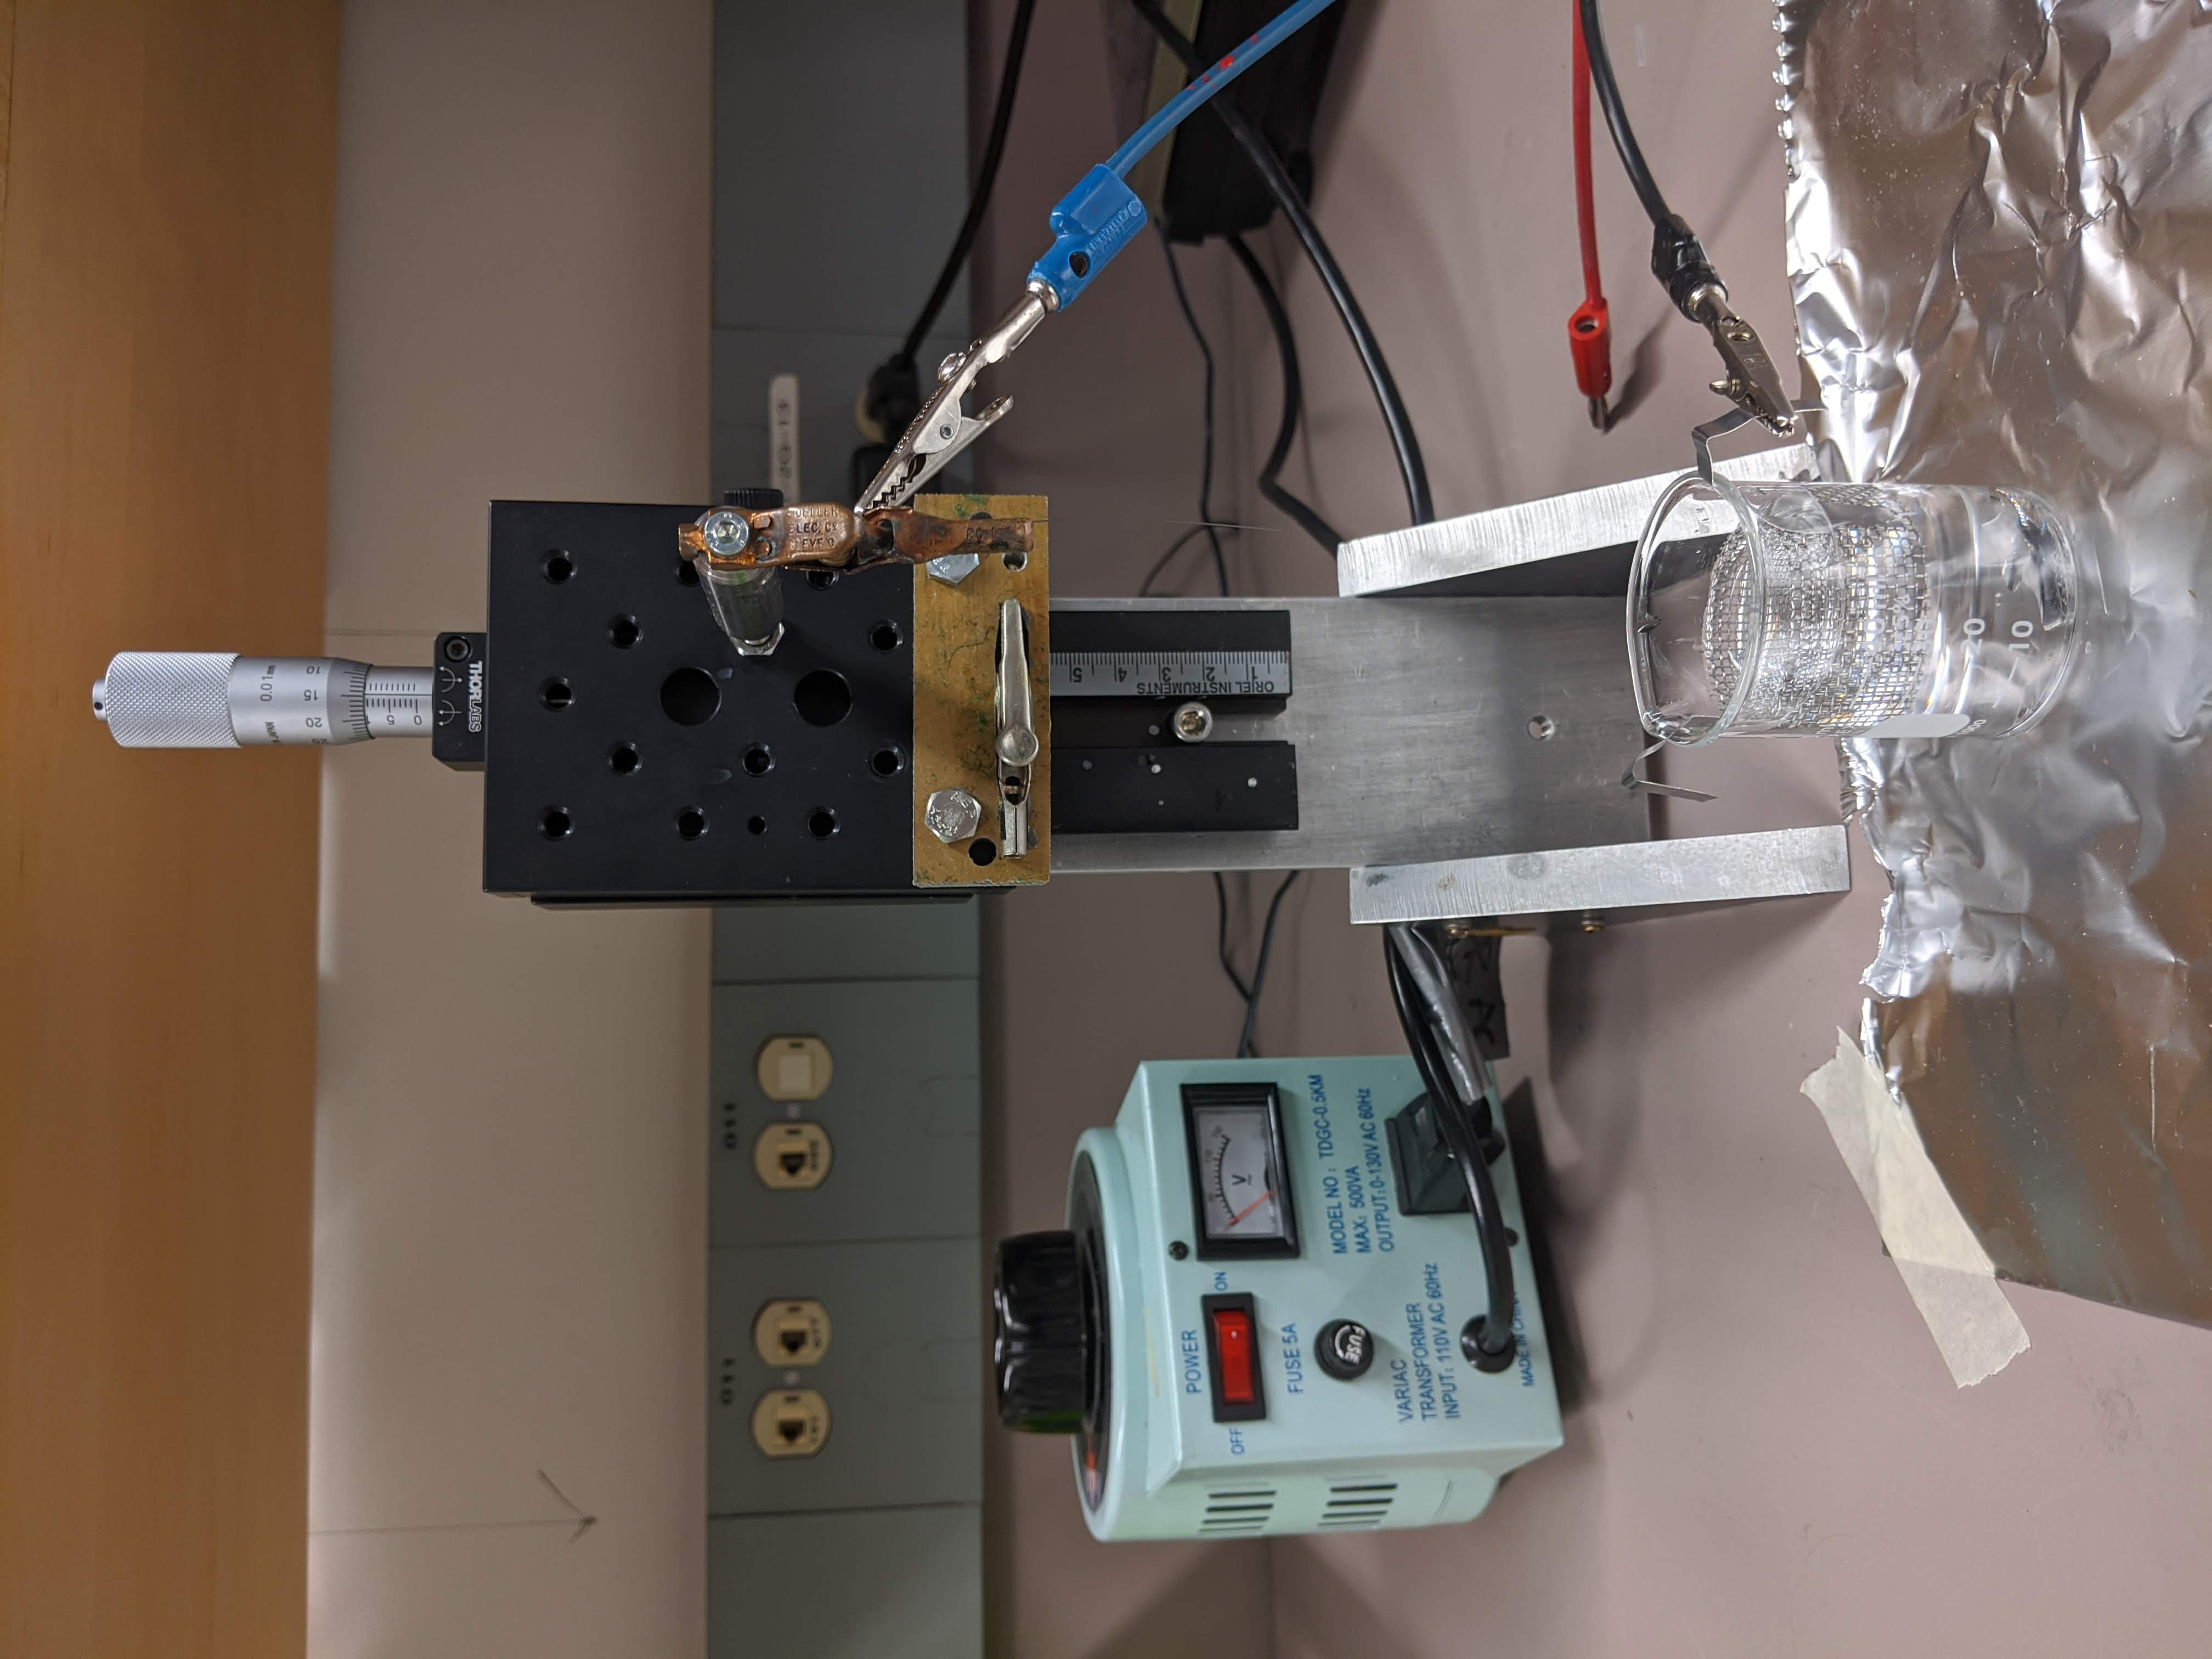
\includegraphics[width=3in,angle=-90]{pictures/etching.jpg}
    \caption{\FIXME{show the fragmented images}}
    \label{fig:oled:hmat-frag}
\end{figure}

Fortunately, intact molecules were found with still attached functional groups. The molecules were scanned, and a pixel-by-pixel \ac{STS} grid was performed on the molecules on Ag(111). Taking the normalized differential conductance, the \ac{LDOS} was plotted as a function of energy, and the \ac{HOMO} and \ac{LUMO} orbitals were visualized spatially. \ac{DFT} calculations were performed for each of the \ac{HMAT} derivative molecules, and used as comparison to the experimental results. The results for HMAT-O, HMAT-TZ, and HMAT-HZ are shown in Figures \ref{fig:oled:hmat-o}, \ref{fig:oled:hmat-tz}, and \ref{fig:oled:hmat-hz}, respectively. 

\begin{figure} [h]
    \centering
    %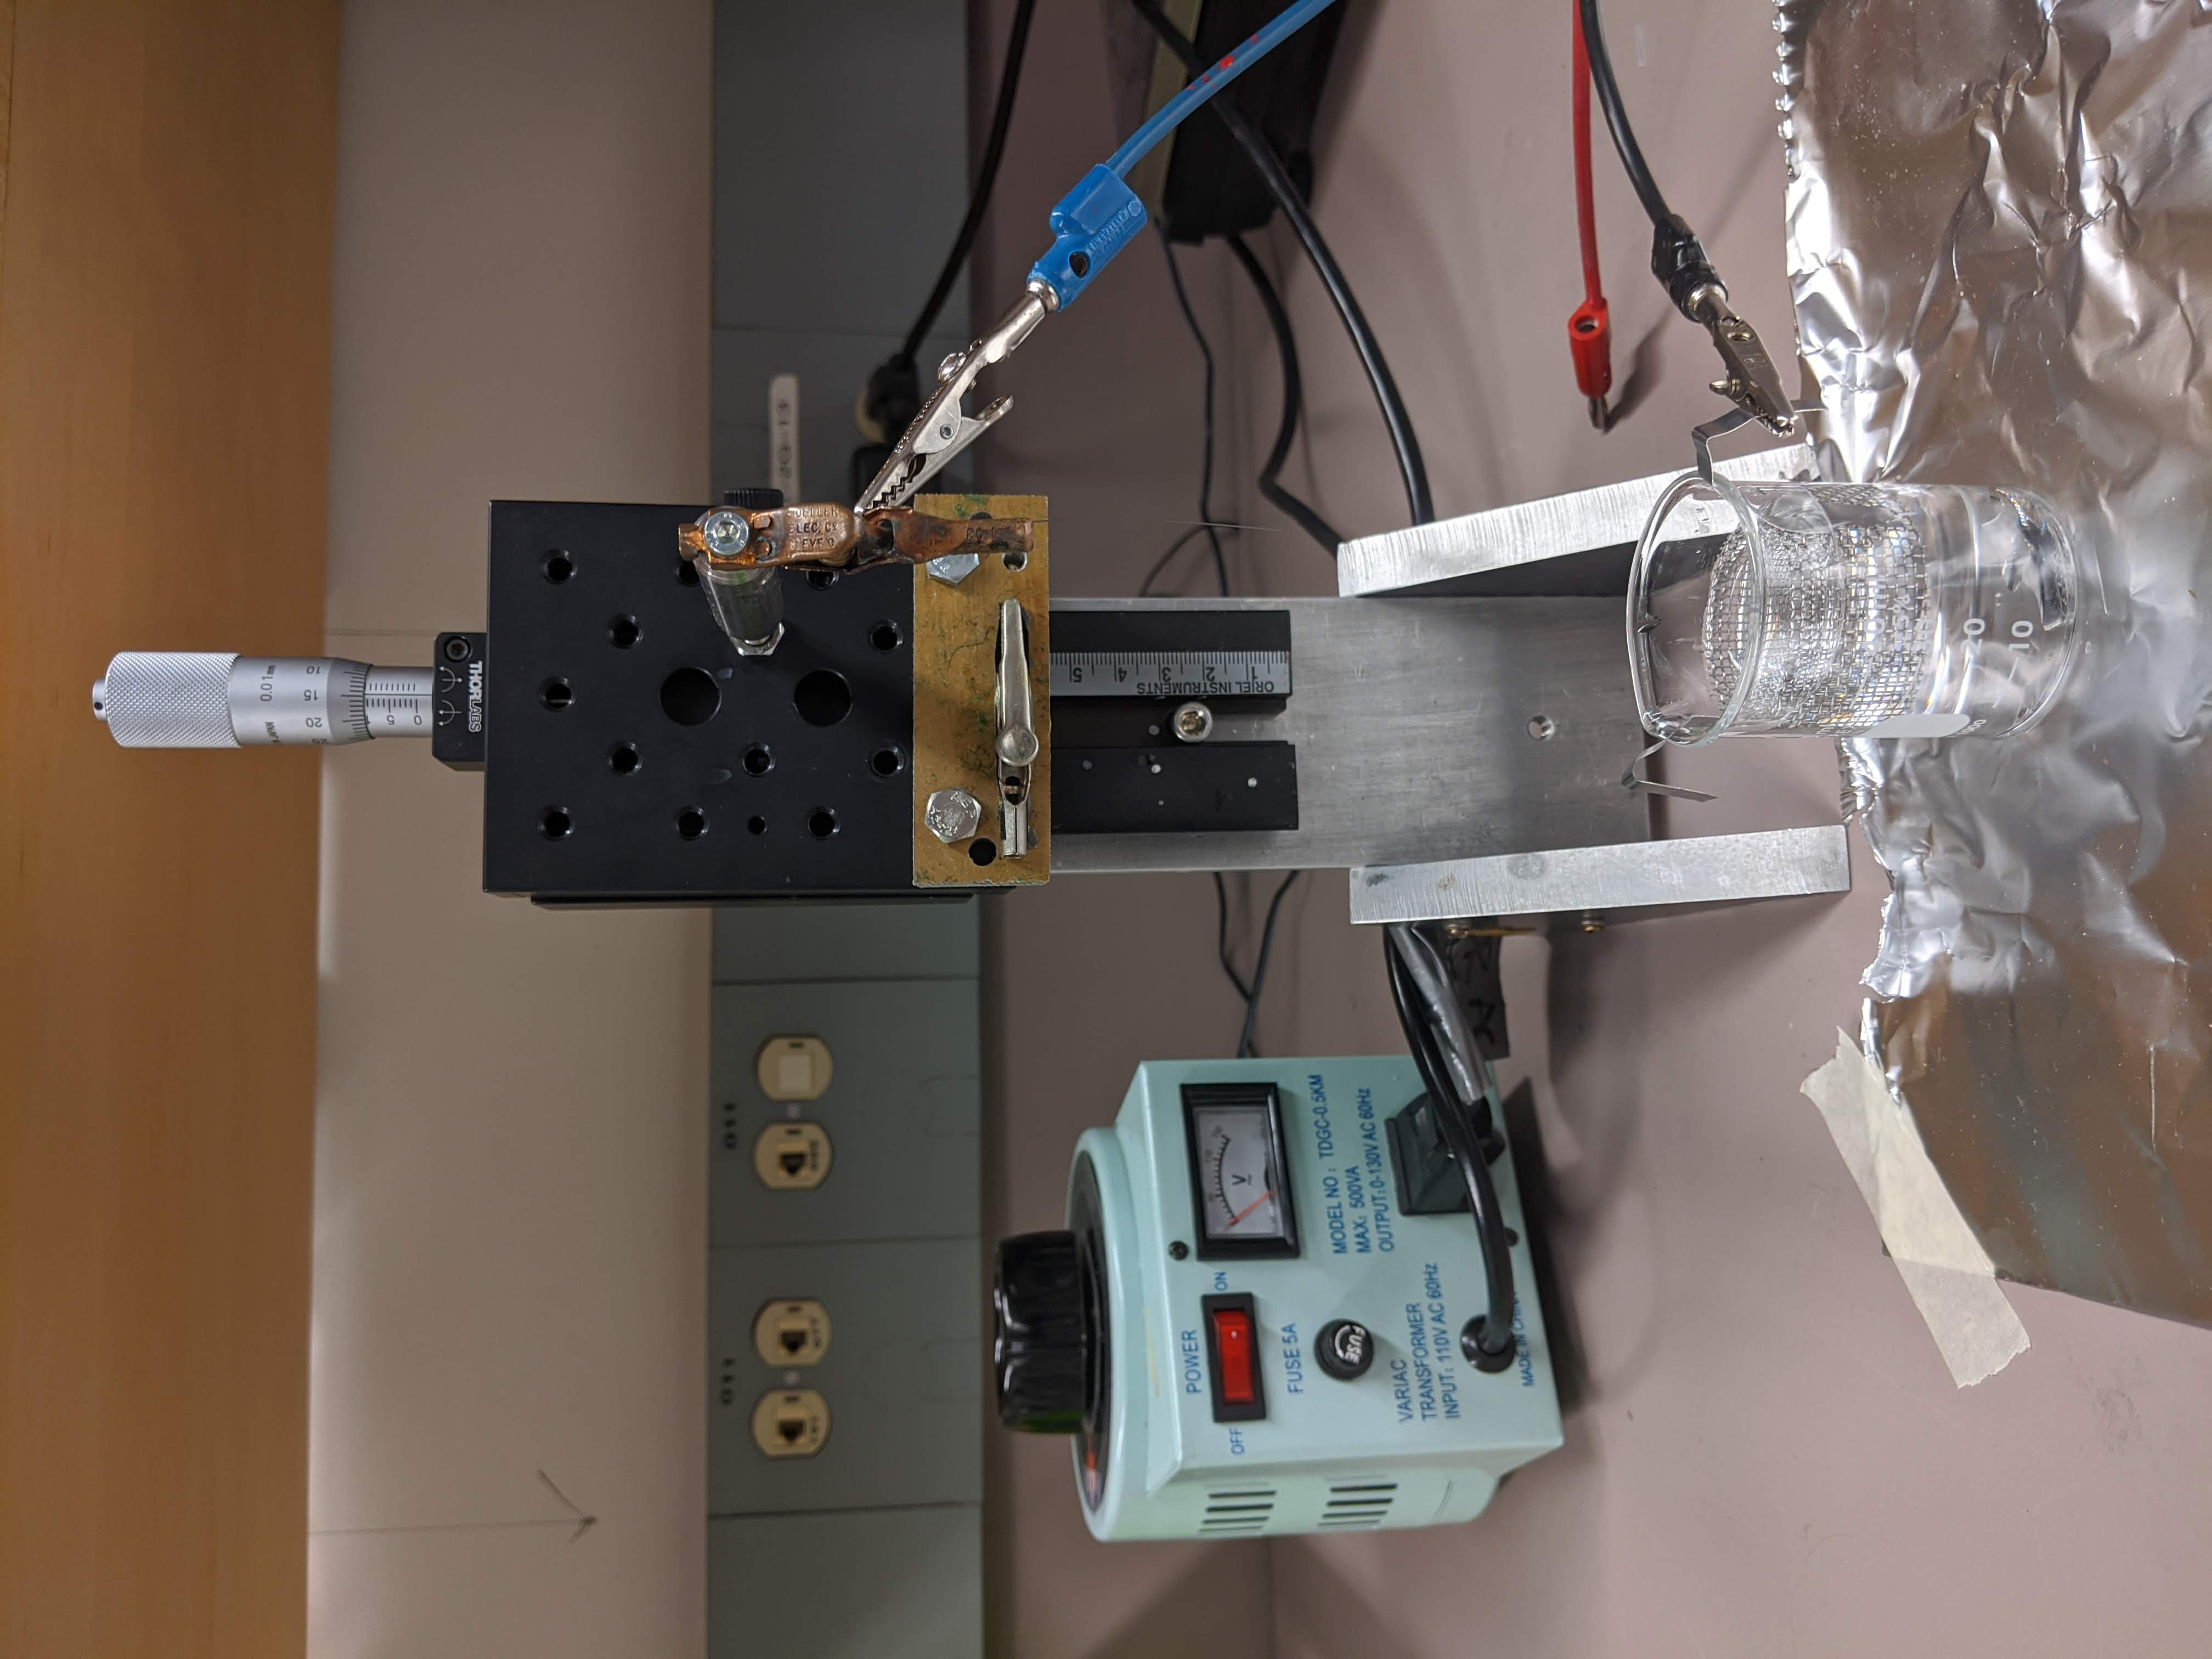
\includegraphics[width=3in,angle=-90]{pictures/etching.jpg}
    \caption{\FIXME{show the fragmented images}}
    \label{fig:oled:hmat-o}
\end{figure}

\begin{figure} [h]
    \centering
    %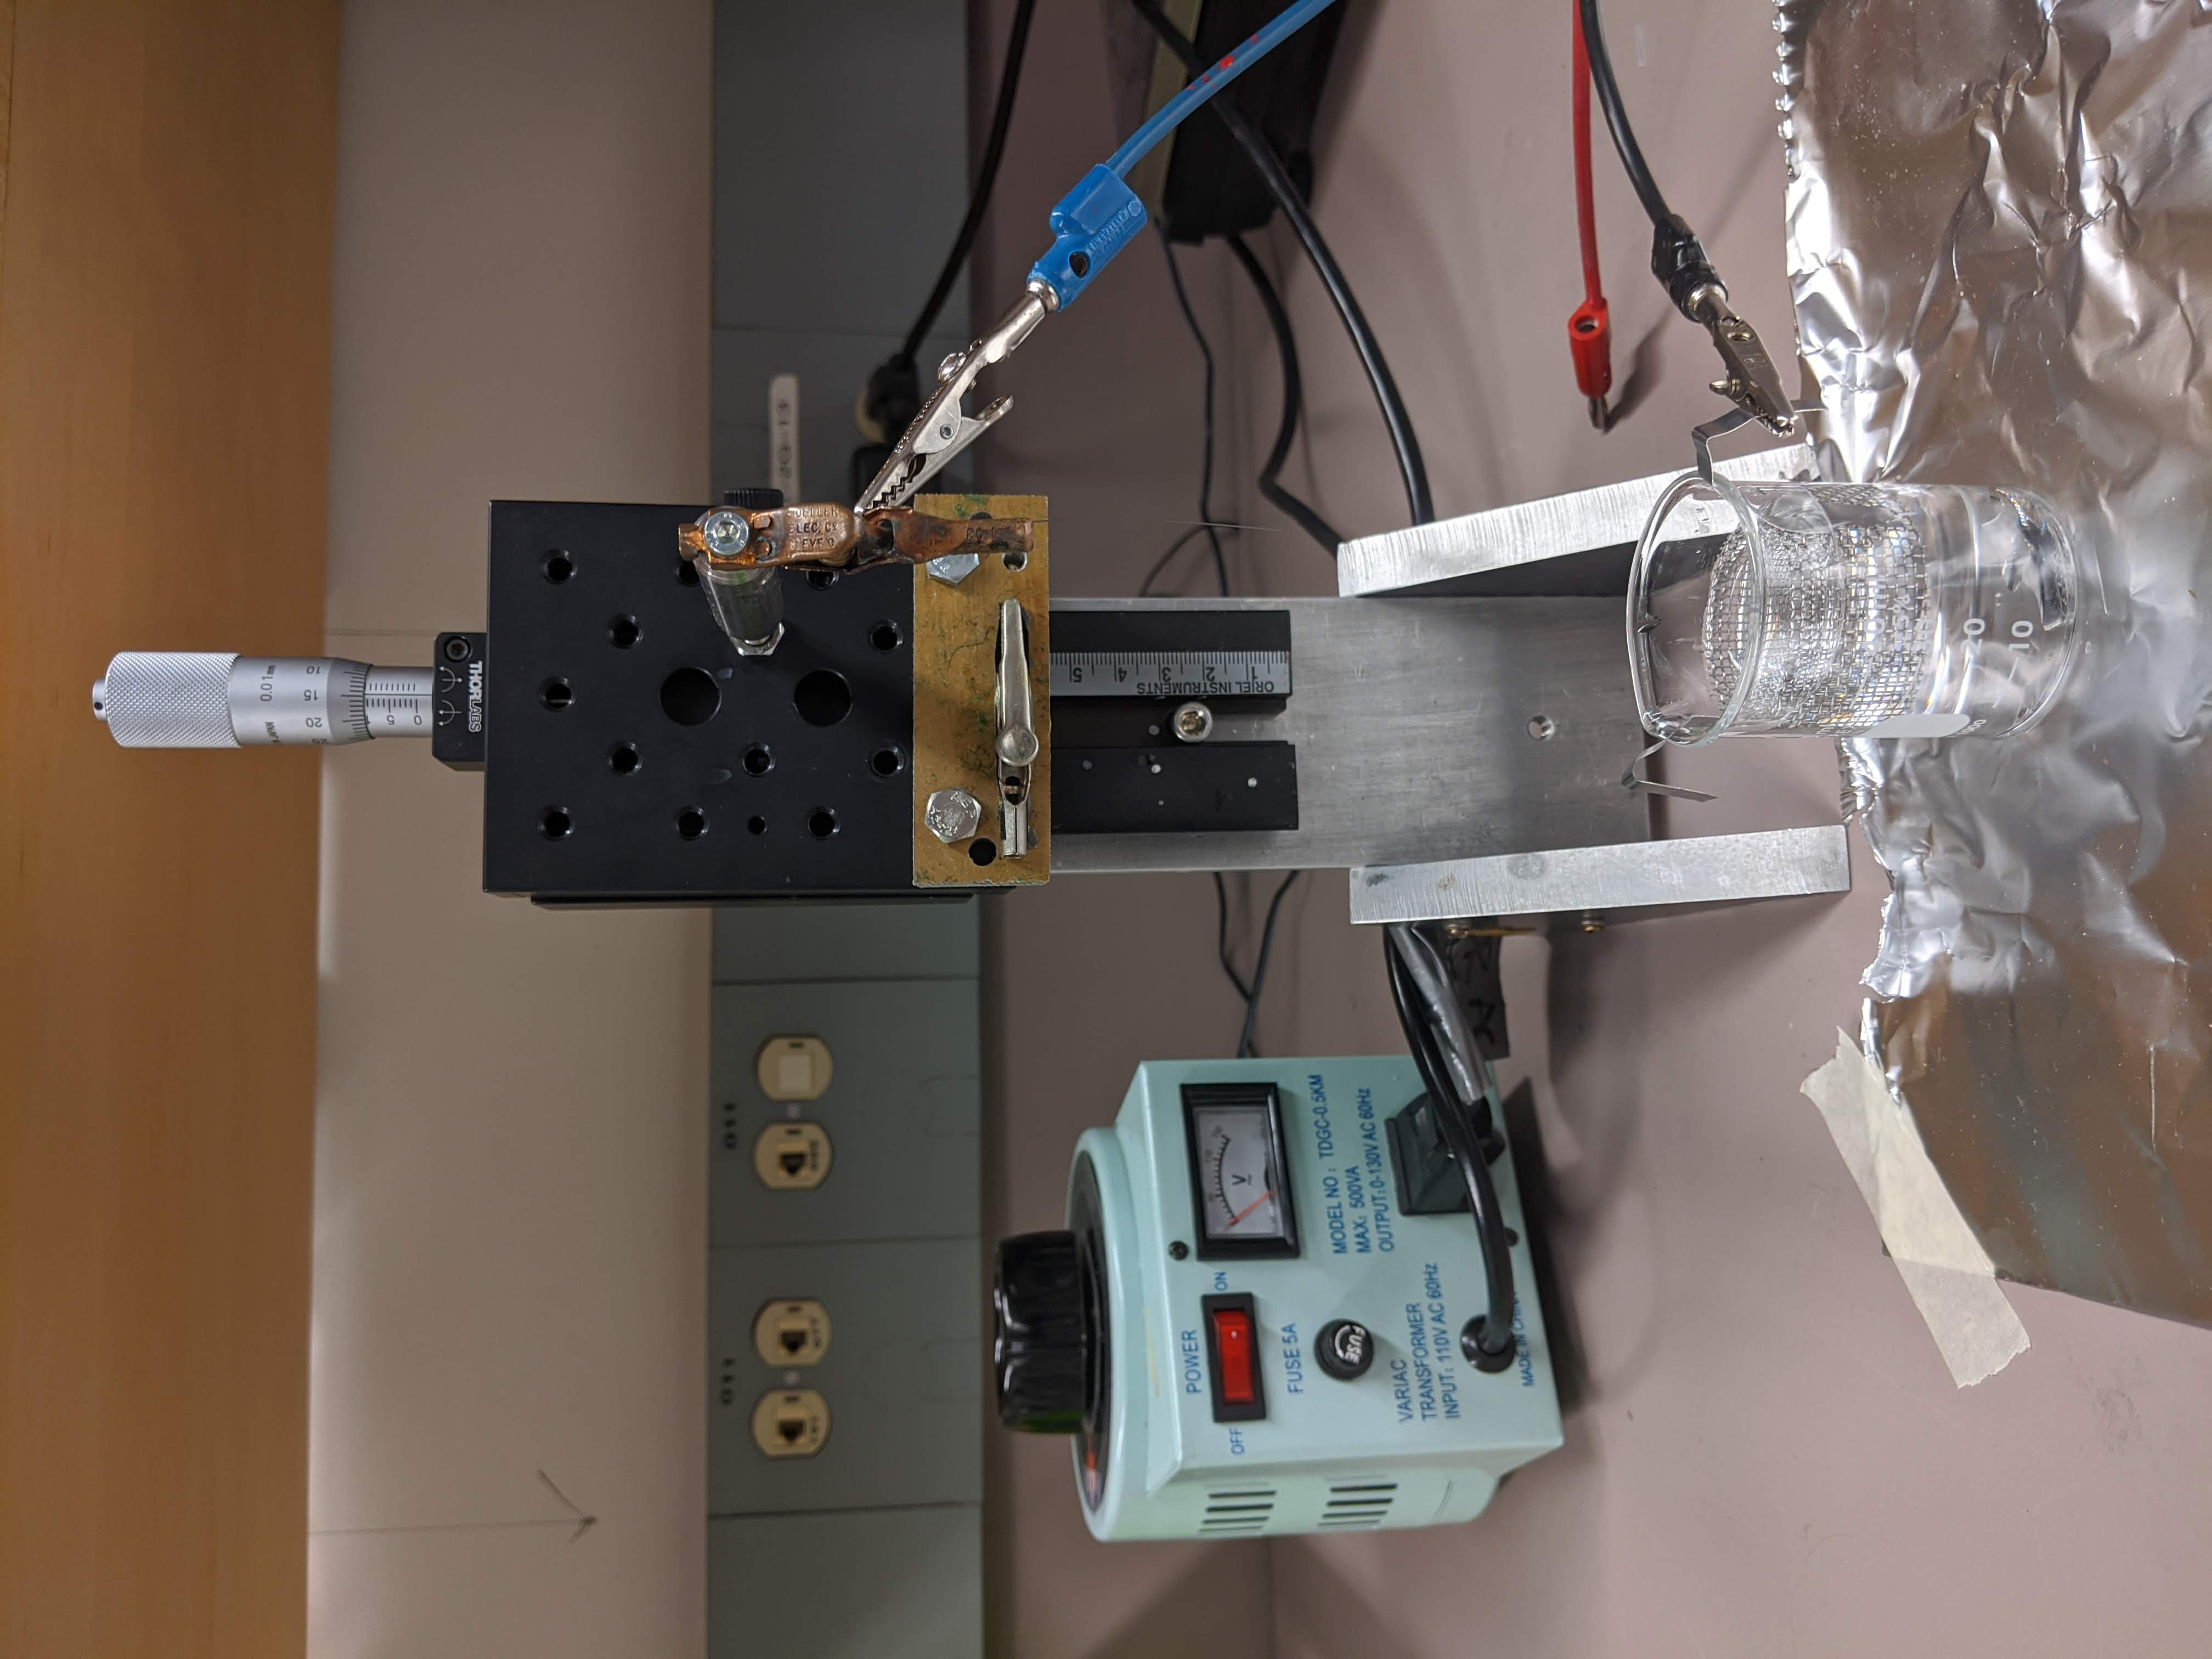
\includegraphics[width=3in,angle=-90]{pictures/etching.jpg}
    \caption{\FIXME{show the fragmented images}}
    \label{fig:oled:hmat-tz}
\end{figure}

\begin{figure} [h]
    \centering
    %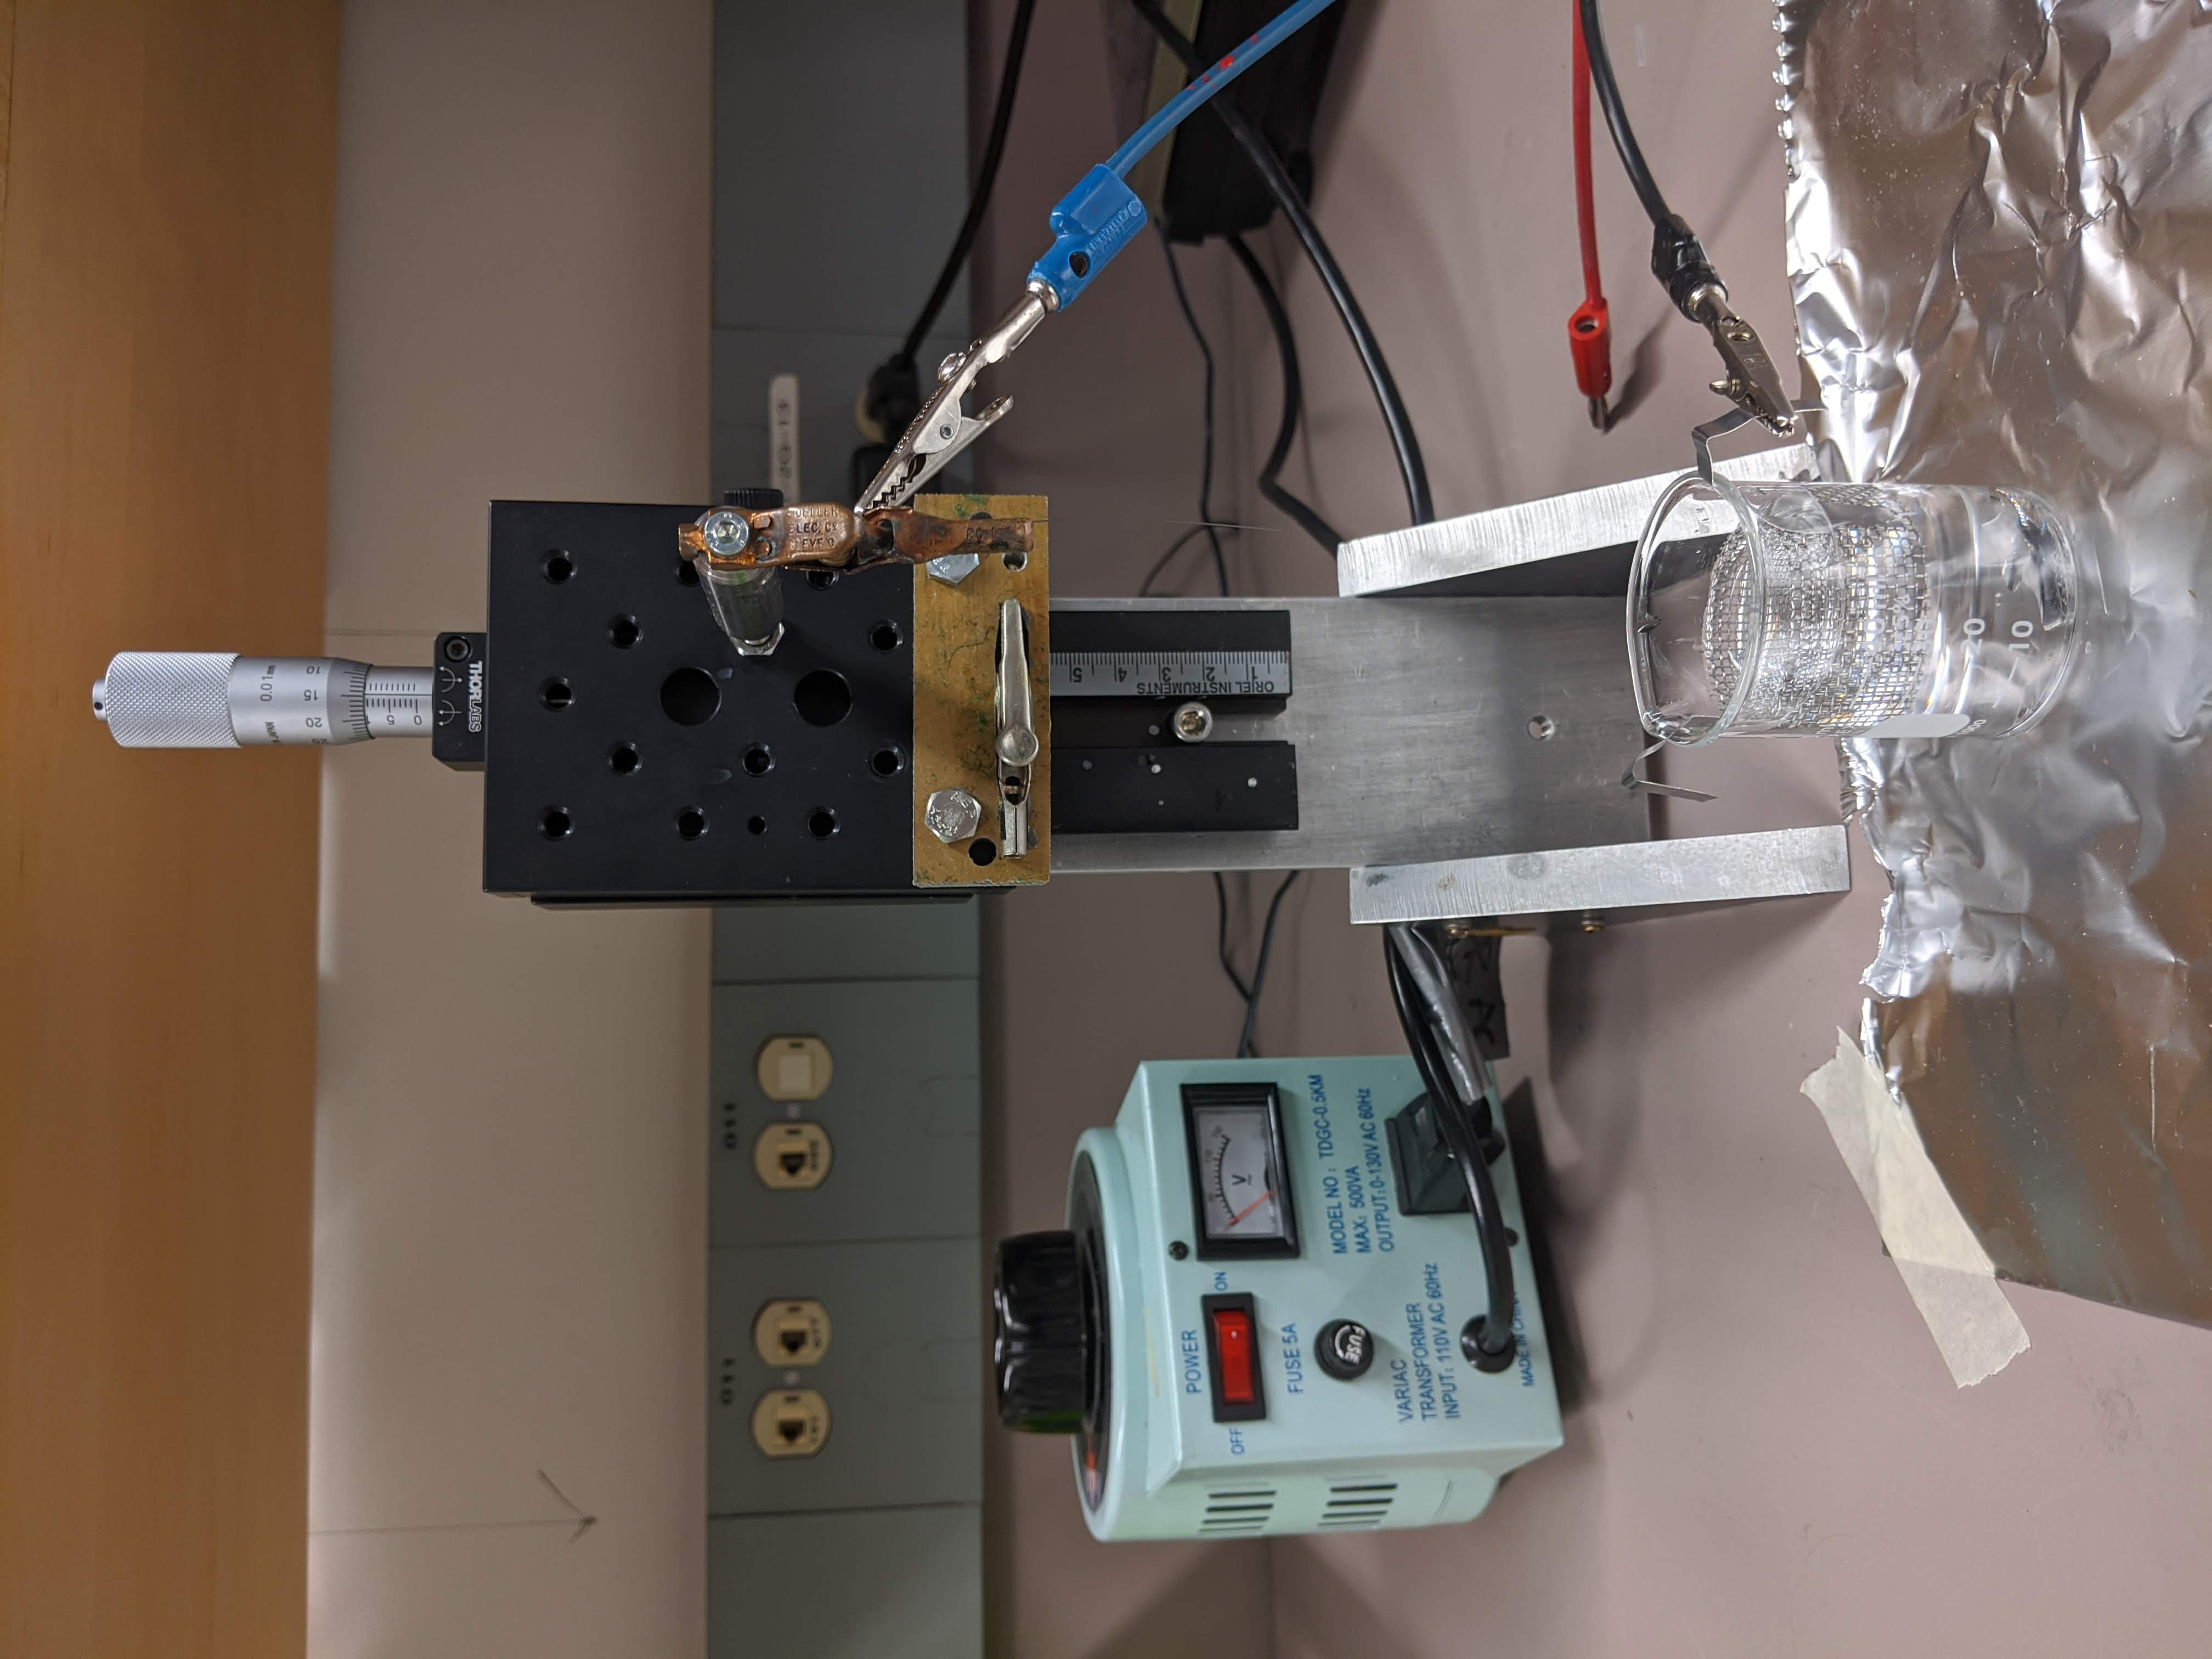
\includegraphics[width=3in,angle=-90]{pictures/etching.jpg}
    \caption{\FIXME{show the fragmented images}}
    \label{fig:oled:hmat-hz}
\end{figure}

For each of the molecules, there is qualitative agreement in the molecular orbital distribution between the \ac{STS} and the \ac{DFT}---the \ac{HOMO} state is localized on the \ac{HMAT}, while the \ac{LUMO} state is localized on the acceptor group. In the case of \ac{HMAT-HZ}, the LUMO and the LUMO+1 were both imaged in \ac{STS}, and, as seen in the \ac{DFT} result, both were localized primarily on the heptazine.

The experimental and theoretical band gaps for each molecule are summarized in \autoref{tab:oled:bandgaps} and \autoref{fig:oled:bandgap-diagram}. The exact band gap energies do not correspond between \ac{DFT} and \ac{STS}. This is expected, as the \ac{DFT} calculations do not account for the interactions between the molecule and substrate. The \ac{STS} experiments were performed without an insulating NaCl layer, so the molecular orbital energies experience significant shifts.

\begin{table} [h]
\begin{center}
    \begin{tabular}{|c|c|c|} 
    \hline
        Molecule  &  DFT band gap (eV)  &  STS band gap (eV) \\
        \hline
        HMAT     &    4.45   &  --- \\
        HMAT-O   &    3.45   & 3.95 \\
        HMAT-TZ  &    3.28   & 2.60 \\
        HMAT-HZ  &    2.54   & 2.45 \\
        \hline
    \end{tabular}
    \caption{\FIXME{caption this, values may be different with norm didv}}
    \label{tab:oled:bandgaps}
    \end{center}
\end{table}

In both the \ac{DFT} and \ac{STS}, there is a clear trend in the HOMO-LUMO gap of each of the \ac{HMAT} derivatives. With the addition of increasingly electronegative species (with increasing number of \ch{O} and \ch{N} atoms), the electron affinity of the molecule increases, and the \ac{LUMO} is lowered in energy (\autoref{fig:oled:bandgap-diagram}). The \ac{HOMO} experiences no shift in energy relative to the Fermi level.

\begin{figure} [h]
    \centering
    %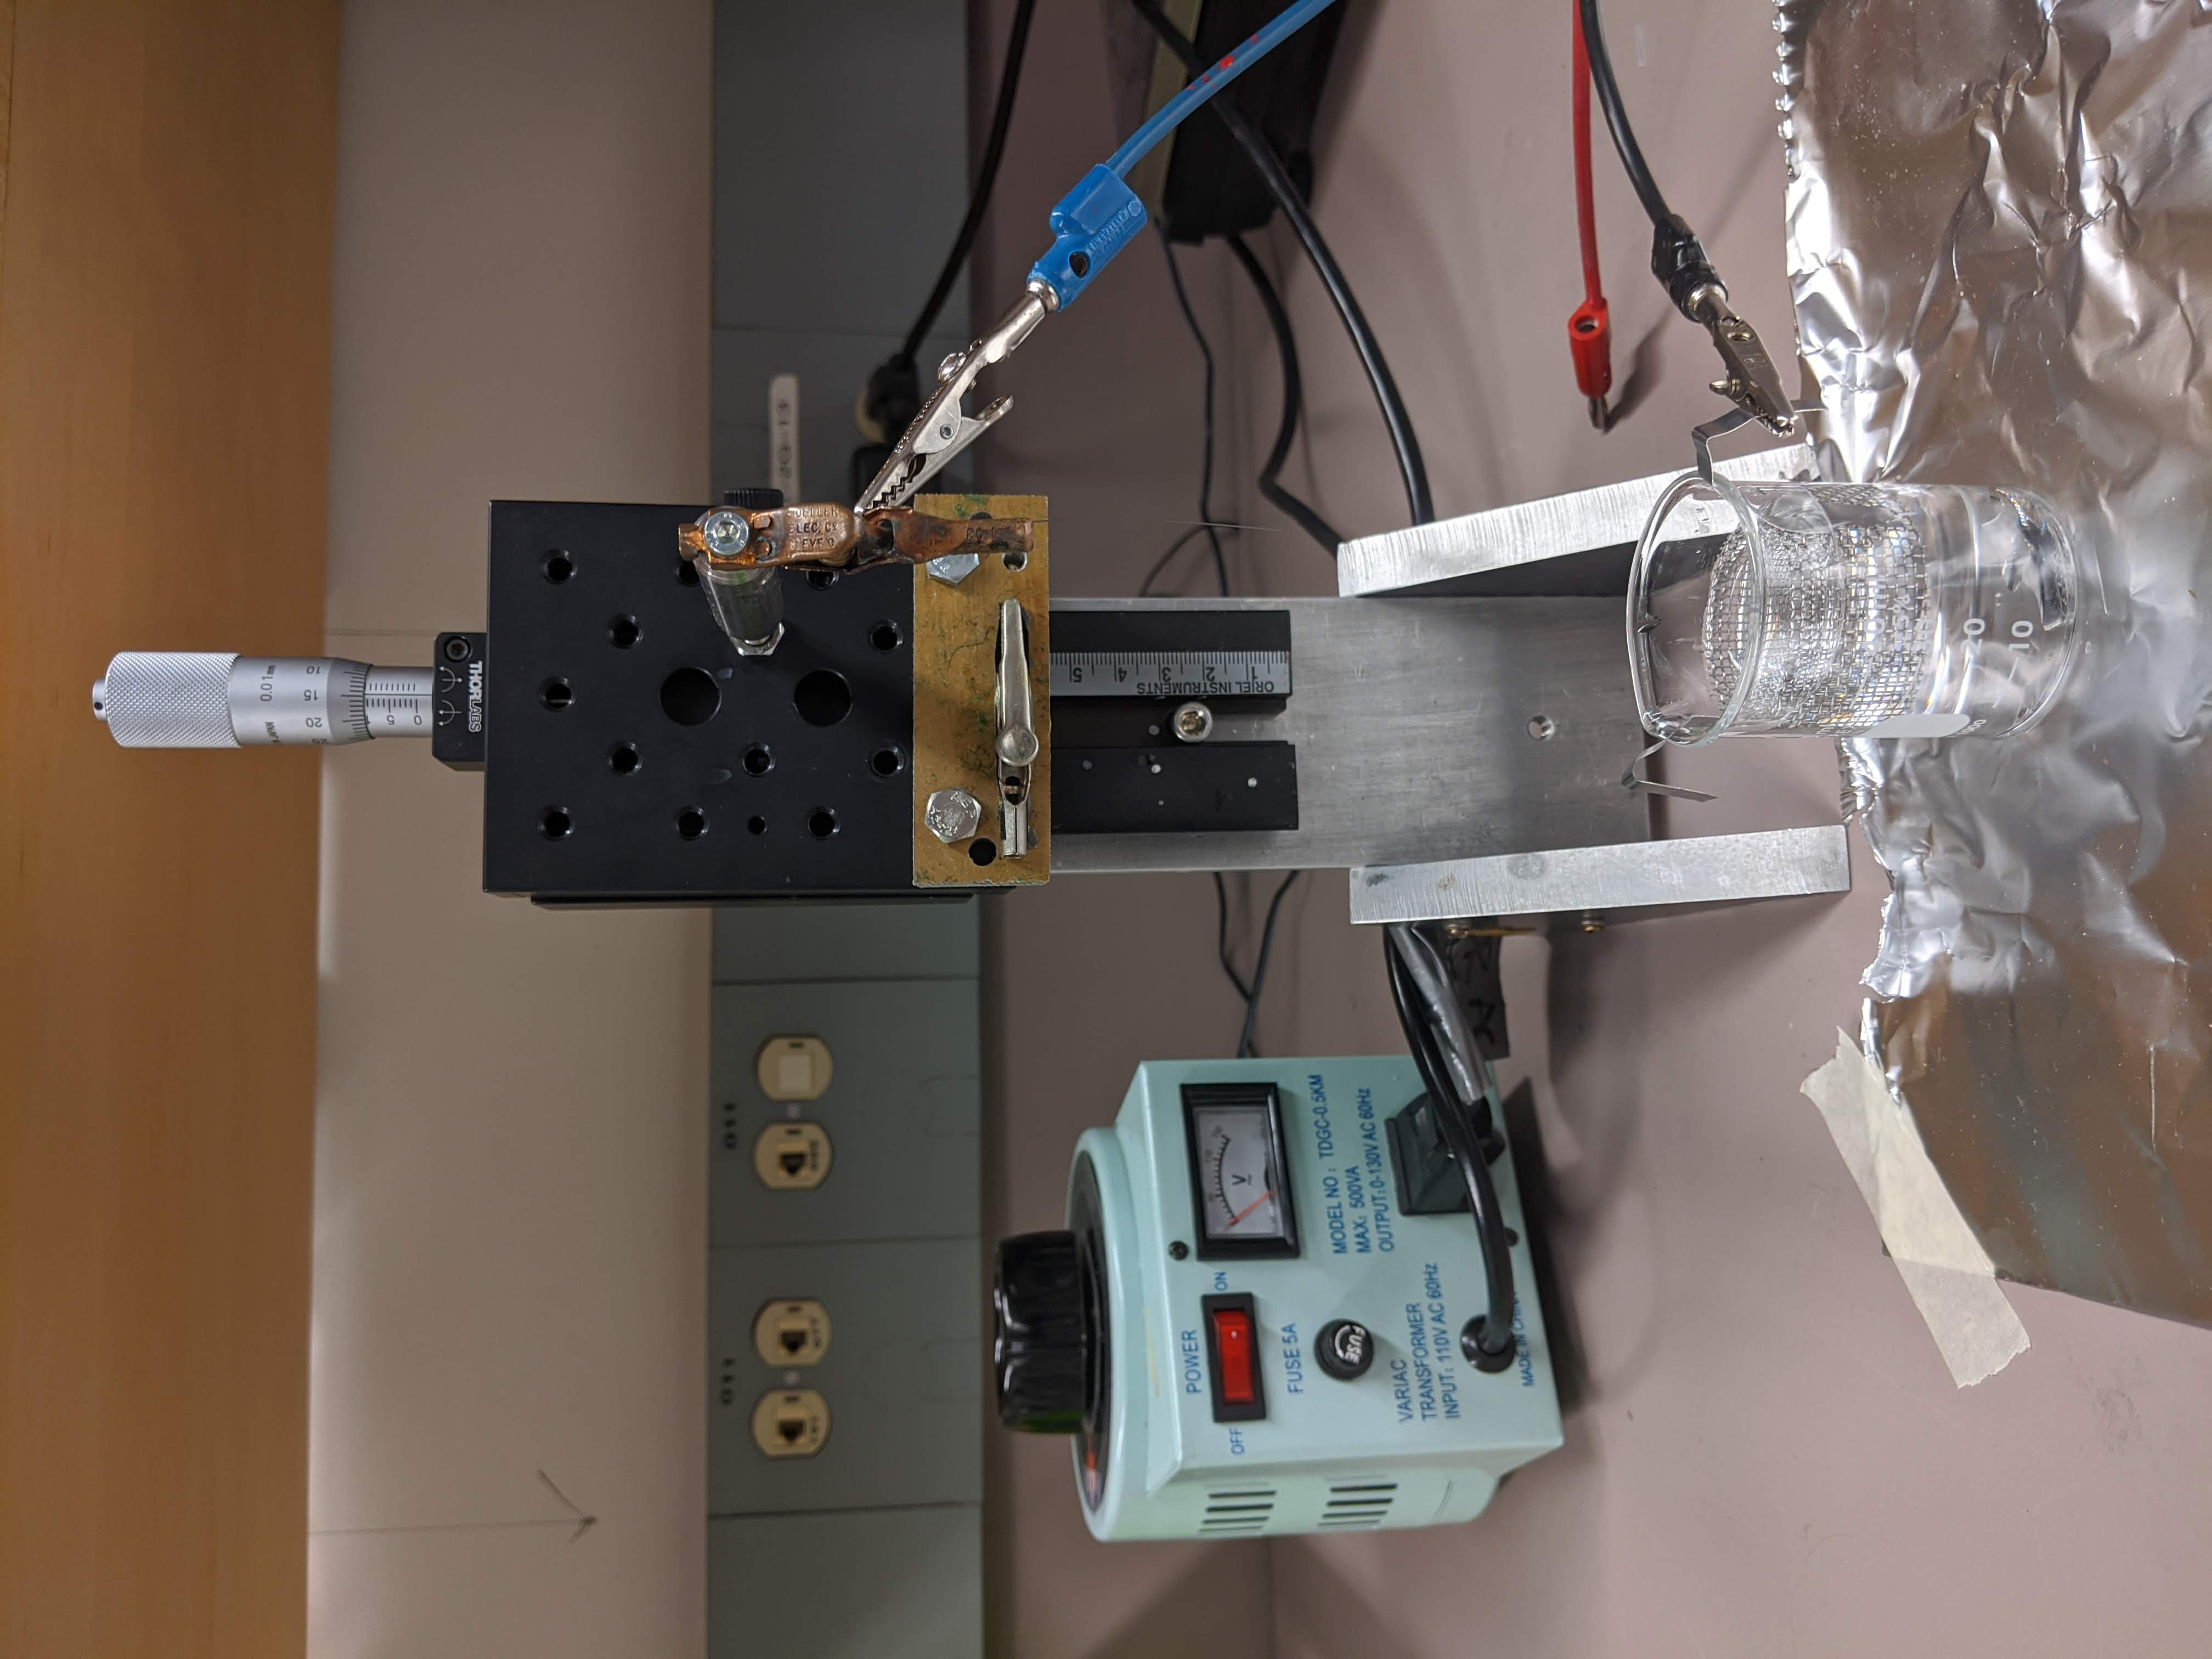
\includegraphics[width=3in,angle=-90]{pictures/etching.jpg}
    \caption{\FIXME{band gap shrinking diagram}}
    \label{fig:oled:bandgap-diagram}
\end{figure}

No attempts were made to perform \ac{SPM} on these molecules on an insulating NaCl layer due to the fragility and instability of the molecules at higher biases. At tip-sample biases $|V_b| > \SI{2.5}{V}$, the molecules would shift on the surface, and the bonds between the \ac{HMAT} and the functional groups occasionally dissociated. The decoupling of the molecules from the substrate would have resulted in larger band gaps, meaning the molecular orbitals would likely not have been accessible by \ac{SPM}.



\section{\ac{STML} study of HMAT derivatives}

While the molecules were not dissociated from the substrate by a bilayer of NaCl, \ac{STML} was attempted for \ac{HMAT-O} and \ac{HMAT-HZ}. With successfully resolved molecular states in the \ac{STS}, we hypothesized that the bulky methyl groups (six on each \ac{HMAT}) may have sterically disscoiates the molecule from the underlying Ag(111).

However, with the Ag tip parked on the molecule at parameters up to \SI{3}{V}/\SI{200}{pA}/\SI{360}{s}, no molecular luminescence was detected, only the plasmonic emission. We also attempted to obtain an absorption spectra by exciting plasmonic photons near the molecule, a technique demonstrated in the past on ZnPc \cite{zhang2017sub}, but again, only the plasmonic emission was seen. The same experiments were repeated on Au(111), in an attempt to redshift the plasmon emission so as to observe the two-photon absorption of the molecules. In all our experiments, no observable \ac{STML} molecular signatures were found from the HMAT-O or HMAT-HZ directly adsorbed on either Ag(111) or Au(111). 

These failed attempts illustrate the importance of dissociation of the molecule from the substrate in \ac{STML}. Metal-molecule coupling results additional energy pathways that rapidly quench excited states, and any emission signal from the molecule. Additionally, the instability and large band gaps of \ac{HMAT} derivatives make it difficult to inject charges into the electronic orbitals, or to generate high energy plasmonic emissions to form excitons in the material, without the molecules breaking or moving. \FIXME{Include ideal molecule?}




%%%%%


% Generally recommended to put each chapter into a separate file
%\include{relatedwork}
%\include{model}
%\include{impl}
%\include{discussion}
%% The following is a directive for TeXShop to indicate the main file
%%!TEX root = diss.tex

\chapter{Conclusion}
\label{ch:conc}

%%%%%

Molecular emission was successfully detected in our experiments, demonstrating that our system is capable of \ac{STML} experiments. In our studies of \ac{ZnPc}, broad molecular photoluminescence signals were observed at positive biases. The signals differ from previously reported \ac{STML} on the molecule at negative biases. As the molecules were more mobile when scanned at high positive bias, it is possible that the stability and motion of the molecules on the surface can affect the photon emission process. Other explanations include the presence of an alternate pathway for exciton generation, such as photon-mediated, or the tunnelling into higher energy unoccupied orbitals, such as LUMO+1. Signals detected in our study of \ac{PTCDA} are the first reported single molecule emission on uncharged \ac{PTCDA}. Similar to the emission detected on \ac{ZnPc}, the experiment was conducted at positive bias, and the detected emission peak was broad.

The effects of fluorination on the photoluminescence of ZnPc were studied through the \ac{SPM} of \ch{F8ZnPc}. \ac{STML} was detected at a bias of \SI{-2.5}{V}, similar to parameters of previously reported \ac{STML} on ZnPc. However, photon emission detected on \ch{F8ZnPc} varied in wavelength from 630\SI{-640}{nm} for different \ch{F8ZnPc} on the surface. \ac{STM} scans at negative biases revealed a variety of topographically different molecules, and point \ac{STS} on the molecules showed differing \ac{LDOS} resonances for the molecules. Repeated sample preparation and replacing of molecules ruled out the presence of degraded molecule, and the switching between molecular species through tip manipulation seemed to indicate that the variety was due to changes in surface adsorption of the molecules. Molecules with smaller band gaps in the \ac{STS} spectra produced lower energy emission peaks in the \ac{STML} spectra, demonstrating correlation between the shifts in electronic states and the optical gap of formed excitons.

After a full system bake-out, a new sample was produced, and the variety of \ch{F8ZnPc} was observed again. However, the sample was noticeably different, with fewer defects on the NaCl bilayers, and new types of \ch{F8ZnPc} observed than those of the sample used for \ac{STML}. Regardless, the different types of molecules were categorized by \ac{STS} spectral features, \ac{STM} topographic differences, and relative positions on the NaCl lattice. We conclude that the presence of the fluorines in \ch{F8ZnPc} stabilize certain adsorption geometries not observed for ZnPc. These changes in conformation and interactions with the substrate can affect the electronic and optical properties of the molecules.

In our study of HMAT derivatives, using pixel-by-pixel \ac{STS}, sub-molecular images of the molecular orbitals for each HMAT molecule were generated. We find that the HOMO was localized around the donor complexes, the HMAT groups, of the molecules, while the LUMO was localized around the acceptor complexes. With the functionalization of increasingly electronegative acceptor groups, the band gaps obtained through \ac{STS} were observed to decrease, demonstrating the tuning of electron energy levels in molecules through chemical design. The results observed in our experiments qualitatively agree with DFT calculations of the HMAT derivatives in gas phase. \ac{STML} experiments were attempted for the HMAT derivatives, however, due to the large band gap, high biases would be required to generate excitons in the material, which could break or move the molecules on the surface.




\section{Future directions}

% talk about the new windows
% talk about using a photomultiplier
% talk about mounting a proper height crystal of Au(111).
With the installation of wider bandwidth filter windows in our \ac{SPM}, reproduction of experiments described in the thesis may be worthwhile, as the cutoff and broadening effects of the IR Filter windows would be eliminated in future \ac{STML} experiments. For further improvements, all samples used for \ac{STML} should be at the correct height for maximum emission collection by the \textit{in situ} lens. Additionally, a photomultiplier tube can be installed in place of the spectrometer. With software improvements, the position of the tip can be synchronized with the photomultiplier tube signal to give sub-molecular photon maps of molecular photoluminescence.

The broad emission peaks in our positive bias \ac{STML} studies remain unexplained. In the thesis, several explanations have been provided, but additional experimentation may reveal the exact emission mechanism, and explain the divergences from previously reported results. In particular, the hypothesis of excitons formed by tunnelling into the LUMO+1 of uncharged \ac{PTCDA} may be tested by mapping out the LUMO+1 using bias dependent \ac{STML}. To test whether the stability of molecules at higher biases have an effect on the observed emission, \ac{STML} experiments can be carried out on \ac{ZnPc} or \ac{PTCDA} ``anchored" to features such as defects or step edges on the surface. 

Future experiments can be directed to the study of systems of organic semiconductors on the surface. By annealing the sample, molecules can self-assemble into dimers. The effects of molecule-molecule interactions, such as polarization and charge transfer, on the formed exciton can be examined by \ac{STML} on the dimerized molecules. Additionally, heterodimers of different molecules, such as PTCDA-ZnPc or ZnPc-\ch{F8ZnPc}, can be studied as simplified models of device heterojunctions. Successful formation of ZnPc-\ch{F8ZnPc} dimers have already been demonstrated on (2ML)NaCl/Au(111), as seen in \autoref{fig:conclusion:f8znpc_znpc_dimer}. 

\begin{figure}[H]
    \centering
    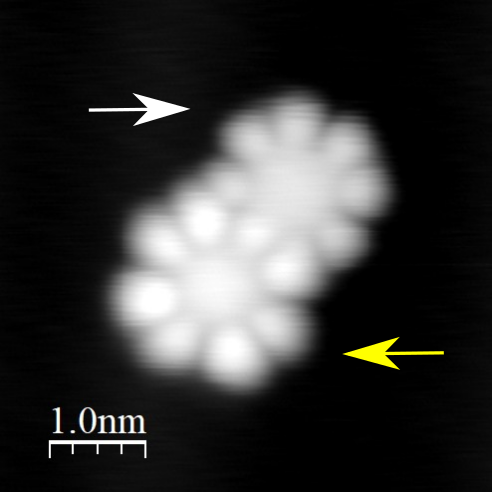
\includegraphics[width=0.5\textwidth]{pictures/f8znpc_znpc_dimer_arrows.png}
    \caption{\sloppy STM image of dimerized \ch{F8ZnPc} and ZnPc on (2ML)NaCl/\-Au(111) (\stmparams{5}{5}{-2.5}{5}). The white and yellow arrows indicate the \ch{F8ZnPc} and ZnPc, respectively.}
    \label{fig:conclusion:f8znpc_znpc_dimer}
\end{figure}

In our study of \ch{F8ZnPc}, we have demonstrated that adsorption geometry can change the electronic structure of the molecule. Separately, we have demonstrated that the change in electronic structure correlates with change in the exciton optical gap. Due to variations in the samples, we cannot make conclusions between the types of \ch{F8ZnPc} observed and the \ac{STML}. A future direction would be to examine the molecules on cleaner NaCl bilayers with the Ag tip, giving simultaneous \ac{STS} and \ac{STML} measurements. Furthermore, theoretical simulations of adsorption geometries of \ch{F8ZnPc} on (2ML)NaCl/Ag(111) may give information on the role of the fluorine atoms on the conformation of the molecule, and resulting changes in molecular orbitals.

Future experiments on the HMAT derivatives are limited due to the incompatibility of the molecules to \ac{SPM} on insulating layers on metallic substrates. Nonetheless, experiments on the HMAT molecules have revealed the necessary properties of candidate molecules for further \ac{STML} experiments, such as a planar structure, and HOMO/LUMO states that do not lie further than \SI{3}{V} from the Fermi level. With an appropriate molecular, the effects of chemical design on the excitonic emission can be studied in future \ac{STML} experiments.





                                    

%    3. Notes
%    4. Footnotes

%    5. Bibliography
\begin{singlespace}
\raggedright
\bibliographystyle{unsrtnat}
\bibliography{biblio}
\end{singlespace}

% \appendix
%    6. Appendices (including copies of all required UBC Research
%       Ethics Board's Certificates of Approval)
%\include{reb-coa}	% pdfpages is useful here
% \chapter{Supporting Materials}



% \backmatter
%    7. Index
% See the makeindex package: the following page provides a quick overview
% <http://www.image.ufl.edu/help/latex/latex_indexes.shtml>


\end{document}
